\documentclass{sig-alternate}
%\documentclass{vldb}
%\documentstyle{article}
%\documentstyle[amsmath,amsthm,amssymb,twocolumn]{article}
%\usepackage{times}
\usepackage{mathtools}
\usepackage{epigraph}


%\usepackage{MnSymbol} 
%\usepackage{MinionPro}
%\usepackage[mathlf,textlf,minionint]{MinionPro}
%\usepackage[T1]{fontenc}
%\usepackage{textcomp}
\usepackage{multirow}
\usepackage{times}
\usepackage{pgfplots}
%\usepackage{subfigure}
%\usepackage{amsmath,amssymb}
\usepackage{graphicx,color}
%\usepackage{verbatim}
%\usepackage{framed}
%\usepackage[ruled,vlined]{algorithm2e}
%\usepackage{floatrow}
\usepackage{algorithm}
\usepackage[noend]{algpseudocode}
\usepackage{xspace}
\usepackage[font={small,it}]{caption, subcaption}
\usepackage{paralist}

\usepackage{balance}

\begin{document}



\newcommand{\reviewer}[1]{\textcolor{red}{Review: #1}}
\newcommand{\mpv}[1]{\textcolor{blue}{MV: #1}}
\newcommand{\agp}[1]{\textcolor{magenta}{AGP: #1}}
%\newcommand{\alkis}[1]{\smallskip\noindent \textcolor{red}{\it $\Rightarrow$ Alkis: #1}}
\newcommand{\SeeDB}{{\sc SeeDB}\xspace}
\newcommand{\calQ}{\mathcal{Q}}
\newcommand{\calR}{\mathcal{R}}
\newcommand{\att}[1]{{\text{#1}}}

\newcommand{\calA}{\mathcal{A}\xspace}
\newcommand{\calX}{\mathcal{X}\xspace}
\newcommand{\calY}{\mathcal{Y}\xspace}

\newcommand{\hc}{\hat{c}\xspace}
\newcommand{\htt}{\hat{t}\xspace}



\newtheorem{definition}{Definition}[section]
\newtheorem{example}[definition]{Example}
\newtheorem{problem}{Problem}[section]
\newtheorem{theorem}{Theorem}[section]
\newtheorem{lemma}{Lemma}[section]

\renewcommand{\baselinestretch}{0.995}

%\DeclareMathOperator*{\argmax}{arg\!\max}


\makeatletter
\def\@copyrightspace{\relax}
\makeatother

%\newcommand{\histvis}{\mbox{\sc HistVis}}
\newcommand{\squishlist}{
   \begin{list}{$\bullet$}
    { \setlength{\itemsep}{0pt}
      \setlength{\parsep}{2pt}
      \setlength{\topsep}{0pt}
      \setlength{\partopsep}{0pt}
      \leftmargin=25pt
\rightmargin=0pt
\labelsep=5pt
\labelwidth=10pt
\itemindent=0pt
\listparindent=0pt
\itemsep=\parsep
    }
}
\newcommand{\squishend}{\end{list}}

\newenvironment{denselist}{
    \begin{list}{\small{$\bullet$}}%
    {\setlength{\itemsep}{0ex} \setlength{\topsep}{0ex}
    \setlength{\parsep}{0pt} \setlength{\itemindent}{0pt}
    \setlength{\leftmargin}{1.5em}
    \setlength{\partopsep}{0pt}}}%
    {\end{list}}


\newcommand{\eat}[1]{}
\newcommand{\papertext}[1]{#1}
\newcommand{\techreport}[1]{}

\newcommand{\techreporttext}[1]{}
\newcommand{\stitle}[1]{\vspace{0.25em}\noindent\textbf{#1}}

\newcommand{\srm}[1]{\textcolor{blue}{Sam: #1}}


%\title{{\LARGE \sc SeeDB}: Towards Automatic Query Result Visualizations}
\title{{\LARGE \sc SeeDB}: Supporting Fast Visual Analytics \\ with Intelligent Recommendations}
%\subtitle{\vspace{-10pt}[Vision Paper]\vspace{5pt}}

\numberofauthors{4} 
\author{
\alignauthor
\hspace{-45pt} Manasi Vartak \\ 
\affaddr{\hspace{-45pt}MIT} \\
\affaddr{\hspace{-45pt}mvartak@mit.edu} 
\alignauthor 
\hspace{-95pt}Samuel Madden \\ 
\affaddr{\hspace{-95pt}MIT} \\ 
\affaddr{\hspace{-95pt}madden@csail.mit.edu}
\alignauthor
\hspace{-120pt}Aditya Parameswaran \\ 
\affaddr{\hspace{-120pt}University of Illinois (UIUC)} \\
\affaddr{\hspace{-120pt}adityagp@illinois.edu} 
\alignauthor 
\hspace{-145pt}Neoklis Polyzotis \\ 
\affaddr{\hspace{-145pt}Google} \\ 
\affaddr{\hspace{-145pt}alkispolyzotis@gmail.com} 
}
 
%\numberofauthors{3}
%\author{
%}

\maketitle
 \begin{abstract}
 %!TEX root=document.tex


Data analysts operating on large volumes of data often rely on visualizations to
interpret the results of queries.
However, finding the right visualization given a query of interest is a
laborious and time-consuming task.
We propose \VizRecDB, a system to partially automate this task:
given a query, \VizRecDB\ intelligently explores the space of all possible
visualizations, evaluates promising visualizations, and automatically recommends
the most ``interesting'' or ``useful'' visualizations to the analyst.
In this paper, we present two implementations of \VizRecDB\ which make very
different design choices: the first leverages existing database systems as the
backend and aggressively optimizes queries to get the highest performance; the
second is a proof-of-concept implementation that has been engineered from
scratch and, without the constraints of the DBMS API, can overcome many of the
limitations of the first design.
For both implementations, we develop and evaluate a suite of optimizations that
leverage the underlying system properties.
Our experiments on a range of real world and synthetic datasets demonstrate
that our optimizations speed up processing by up to 8-20X in the DBMS-backed
execution engine.
Similarly, our custom engine can achieve a 10-fold speedup by aggressively
pruning low-utility views. We further show that pruning does not adversely
affect the accuracy of views returned.
Together with the DBMS optimizations and pruning heuristics, we demonstrate that
\VizRecDB can be used to recommend interesting views in near-interactive time
scales.
% Our end-to-end experiments also demonstrate that that \VizRecDB\ can be used to
% find interesting visualizations in interactive time scales.
% Finally, we present the results of a user study that evaluates our method for
% interesting visualizations, the relative quality of different distance metrics
% and the \VizRecDB\ system.

 \end{abstract}
 %!TEX root=document.tex

\section{Introduction}
\label{sec:introduction}
\agp{We need to be careful about the use of: analyst vs. user, utility vs. scoring
function, ...}
Data visualization is often the first step in data analysis.
Given a new dataset or a new question about an existing dataset, an analyst builds
various visualizations to get a feel for the data, to find anomalies and outliers, 
and to identify trends and patterns that might merit further investigation. 
However, when working with high-dimensional datasets, identifying visualizations that
show interesting variations and trends in the data is non-trivial:
the analyst must manually specify a large number of visualizations, explore behavior of various
attributes (and combinations thereof), and examine different subsets of data before finally 
arriving at visualizations that they find interesting or insightful.
This need to manually specify and examine every visualization hampers rapid analysis 
and exploration of data.

\agp{Rewrote this to tone down.}

In this paper, we tackle the problem of automatically 
identifying and recommending 
visualizations.  
One of the core challenges is that it is entirely subjective as to
whether a visualization is interesting or not.  
In this paper, we adopt a simple criterion for judging interestingness, 
that a visualization 
may be interesting if it displays 
{\em large deviations from some
reference} (we define this notion more formally below.)
We demonstrate the efficacy of this criterion in this paper via 
user studies. 
Of course, there many other elements that may make a visualization interesting.
Examples include aesthetics (that 
we borrow from prior work~\cite{polaris,Mackinlay:1986:ADG:22949.22950}), 
the particular attributes of the data being presented 
(our interactive tool allows analysts to choose attributes of interest) 
or other kinds of trends in
data (for example, in some cases, a {\it lack} of deviation may be interesting.)  
Thus, while our focus is on visualizations with large deviation, 
we also design a generalized utility metric for evaluating visualization 
quality (in Section 8), and describe how our system is capable of handling
this generalized utility metric for recommending visualizations.

% However, our hypothesis, which we demonstrate
% empirically through user studies, is that many interesting visualizations 
% demonstrate large deviations from some reference data set (we define this notion formally below.)
% Of course, there many other elements that may make a visualization interesting.
% Examples include aesthetics (which we explicitly do not focus on), the particular attributes of the data being
% presented (our interactive tool allows users to choose attributes of interest) or other kinds of trends in
% data (for example, in some cases, a {\it lack} of deviation may be interesting.)  Thus,
% in addition to our focus on visualizations with large deviation, we develop a generalized
% utility metric for evaluating visualization quality, and develop several
% techniques for recommending {\it high utility} visualizations.

\agp{Rewrote this to make stronger.}

Given a utility metric (based on deviation or otherwise),
the goal of recommending visualizations based on this metric 
raises several challenges:
First, even for a modest dataset with a small number
of attributes, the number of  
visualizations that need to be considered is often in the hundreds or thousands.
Even simply generating each of these visualizations can take many hours 
(as we will see in this paper).
Second, evaluating these visualizations for utility requires repeated
computations on the same underlying data, requiring even more time.
Third, recommendations need to made to analysts at interactive speeds,
making it necessary to avoid some computation altogether at the cost
of returning visualizations with slightly lower utilities. 
Dealing with these challenges and trade-offs in designing our system, \SeeDB, is the primary focus of this paper. 

% first, the curse of dimensionality makes the number of possible visualizations very large;
% second, evaluating the utility of each visualization may require re-running computations over the 
% same underlying data; 
% and third, recommendations must be made to users in real-time, and at interactive speeds.


%Our system, \SeeDB, is designed to address all of these challenges.


% The goal of recommending high-utility visualizations brings up several challenges: first,
% the curse of dimensionality makes the number of possible visualizations very large;
% second, evaluating the utility of each visualization may require re-running computations over the 
% same underlying data; 
% and third, recommendations must be made to users in real-time, and at interactive speeds 
% Our system, \SeeDB, is designed to address all of these challenges.

We begin with an illustrative example that explains the \SeeDB use case and motivates our deviation-based
scoring function. 

% In this work, we combine an {\em incremental view pruning} framework with multi-
% query processing techniques to make recommendations in real time.
% As a first step towards crafting a sophisticated visualization scoring function, we adopt
% a deviation-based metric to quantify the utility of visualizations.

% Data visualization is one of the most common techniques for identifying 
% trends and finding anomalies in data.
% However, with high-dimensional datasets, identifying visualizations that 
% effectively present interesting variations or patterns in the data is a non-trivial task:  a
% user typically builds a large number of visualizations optimizing for a range of visualization 
% types, aesthetic features, and more
% before arriving at one that shows something valuable.

% In this paper, we tackle the problem of automatically recommending such valuable visualizations.
% The problem of recommending visualizations is complicated because a ``good'' visualization needs to take into account several different dimensions, including:
% \begin{inparaenum}
% \item types and properties of the different attributes in the dataset ({\it metadata}), 
% \item visual qualities of the visualization ({\it aesthetics}). 
% \item the particular subset of data the user is interested in ({\it query}), 
% \item variation in and distribution of the data itself ({\it data distribution}), 
% \item meaning and relative importance of attributes in the data ({\it semantics}),  and
% \item past history of interactions with this user and other users ({\it user preferences})
% \end{inparaenum}

% Current visualization systems like Spotfire and Tableau have limited capabilities to recommend visualizations --- they only focus on metadata and aesthetics dimensions, following standard visualization best-practices, e.g., choice of appropriate colors,
% rules defining when a bar chart is more appropriate than a trend line, etc.  
% No existing system that we are aware of 
% incorporates insights about the underlying data, or for that matter, any of the other dimensions into its recommendations.

%There is much room for research into leveraging information along the remaining dimensions to make more holistic
%recommendations.



%Data analysts must sift through very large volumes of data 
%to identify trends, insights, or anomalies.  This task often involves the visual inspection of data, 
%Given the scale of data, and the relative ease and intuitiveness of examining data visually,
%analysts often use visualizations as a tool to identify patterns of interest.
%Consequently, visualization software such as Tableau~\cite{}, Spotfire~\cite{} and Many Eyes~\cite{} 
%has seen unprecedented user adoption~\cite{kristi-tech-report}.
%In spite of user friendly software, however, selecting the ``right'' visualization still remains a laborious and 
%challenging task, particularly for novices unfamiliar with the data\mpv{citation?}. 
%As demonstrated by the paper on the Tableau use, majority of an analyst's time is spent in exploring
%different visualizations.
%To alleviate this problem, major visualization software vendors are attempting to incorporate automatic visualization
%recommendations into their software.
%For instance, Spotfire recently launched a ``Recommendations'' module that uses attribute metadata (e.g. type, number of distinct
%values) to suggest some ``best-practice'' visualizations~\footnote{http://spotfire.tibco.com/recommendations}.
%Similarly, Tableau's Show Me capability recommends a chart type (bar chart, map etc.) that is appropriate
%for the particular view of the data~\cite{DBLP:journals/tvcg/MackinlayHS07}.
%Both of these recommendations are straightforward applications of the best practices of visual design~\cite(); 
%neither incorporates insights about the underlying data or prior user history into its recommendations.
% These recommendations use basic metadata about attributes (categorical or numeric, number of distinct values etc)
% to produce simple visualizations that follow best practices of visual design.
%The ultimate vision for such a recommendation module is that given a dataset or a query, the visualization 
%software can study trends in data and previous interactions on that dataset to present to the user the 
%visualizations it deems most valuable.


% \mpv{Should we add a paragraph and schematic of an ideal system, that has an ensemble of models along one or 
% more of the above dimensions to produce a holistic list of recommendations?}

%In this paper, we develop a system that uses a combination of metadata, query, and statistics to 
%provide high quality, data-driven visualization recommendations.
%We envision our model to be used in conjunction with models currently used for recommendation and models that
%leverage context and user history to produce holisitc recommendations.

% \stitle{Data-driven Recommendations in \SeeDB.}
% To this end, in this work, we describe a new visualization recommendation engine we are building called {\it \SeeDB}.
% Eventually, we aim to address all six dimensions of the above list of dimensions by developing a suite of optimization techniques designed to explore
% the entire range of visualizations of a user-supplied data set or query result.  
% As a first step in this paper, we develop a general data-driven deviation-based metric that can capture all six dimensions to a limited extent (see Section~\ref{sec:problem_statement} and Section~\ref{sec:discussion}).  
% We focus on the query and data distribution aspects as a special case:
% these add significant utility, and at the same time significant complexity to 
% the visualization recommendation process,
% and are particularly relevant when an analyst is approaching a dataset 
% for the first time. 
% We leverage lessons from metadata and aesthetics-based recommendation
% generation from prior work.

% However, because metadata and aesthetics based recommendations have been addressed in prior work, in this paper we focus on {\it data-driven} recommendations that use information about data distribution, metadata and the user query to recommend visualizations.
% Such visualizations are particularly appropriate when
% approaching a dataset for the first time, with limited domain knowledge or historical context.

% that identify unusual variations in the result of the user-supplied query as compared to the underlying data.
% consider the inherent variations in the data from a user-supplied query. 
%   that focuses less on the aesthetics of good visualizations, and more
% on developing general techniques that explore the space
%of possible visualizations and recommend those that highlight data variability in the subset of data specified by a user's query.
%Metadata about a dataset, the user's query and information about data distributions can together provide powerful
%information to identify potentially interesting visualizations for the user.
%We call these recommendations {\it data-driven} since they do not draw upon any semantic information about the dataset;
%they are guided by statistics alone.
%We envision these techniques being incorporated into existing visualization systems that allow users to supply context (via, e.g.,
%interaction), and that focus more on the aesthetics of good visualization.
%As mentioned before, since we envision these recommendations to be augmented with context information (along with
%information about aesthetics), we can attack the problem piecemeal.

%Of course,  however, we note upfront
%that {\it there is a variety of ways to quantifying utility and these merit further exploration}.
%\mpv{In fact, we hope that the techniques and framework we describe in subsequent sections may be a general framework 
%into which we can plug in a variety of metrics.}

% deviation-based 

%%%%% VLDB original %%%%%%%

% \stitle{Illustrative Example.}
% Consider a smartphone app analytics team that is tasked with studying the metrics for BadApp, a smartphone app that has
% poor performance and has received a lot of consumer complaints. 
% Suppose that the team uses the AppMetrics database containing metrics such as network usage, 
% power consumption, load times etc.
% Given the large size of the database (millions of records), an analyst will 
% overwhelmingly use visualization software to glean insights into the behavior of BadApp.

% In a typical workflow, an analyst would begin by using the program's GUI or a custom query language to execute the equivalent
% of the following SQL query and pull all BadApp metrics from the database. 
% \noindent 
% \begin{align*}
% & \tt Q \ \ = \ \ SELECT \ * \ FROM \ \  AppMetrics \ \ WHERE  \ Name=``BadApp"
% \end{align*}
% Next, the analyst would use an interactive drag-and-drop GUI interface to visualize various metrics of BadApp.
% For instance, the analyst may visualize average network usage for BadApp, total crashes grouped by session time,
% average load times by carrier, distribution of mobile operating systems, and so on.
% Under the hood, these visualization operations are essentially queries to the underlying data store and subsequent graphing of 
% the results.
% For example, the visualization for average load times by carrier is generated by running an operation equivalent to the
% SQL query (Q') shown below.
% %The result of this query is a two-column table that is very likely going to be viewed as a bar-char~\cite{vql, kristi}.
% Table \ref{tab:staplerX} and Figure \ref{fig:staplerX} respectively show an example of the results of Q' and a potential
% visualization.

% \noindent
% \begin{align*}
% & \tt Q' = SELECT \ \ carrier,\ AVG(load\_time) \ \ FROM \ \  AppMetrics \\
% & \tt \hspace{20pt} WHERE\ Name=``BadApp" \ \ GROUP  \ \ BY \ \ carrier
% \end{align*}

% \begin{figure}[h]
% \vspace{-10pt}
% 	\centering
% 	\begin{subfigure}{0.49\linewidth}
% 	   \begin{tabular}{cc} \hline
% 		  Carrier & Load Times (ms) \\ \hline
% 		  AT\&T & 180.55 \\ \hline
% 		  Sprint & 90.13 \\ \hline
% 		  T-Mobile & 122.00 \\ \hline
% 		  Verizon &  145.50\\ \hline
% 		  \end{tabular}
% 		  \caption{Data: Average Load Times by Carrier for BadApp} \label{tab:staplerX}
% 	\end{subfigure}
% 	\begin{subfigure}{0.49\linewidth}
% 		\centering
% 		{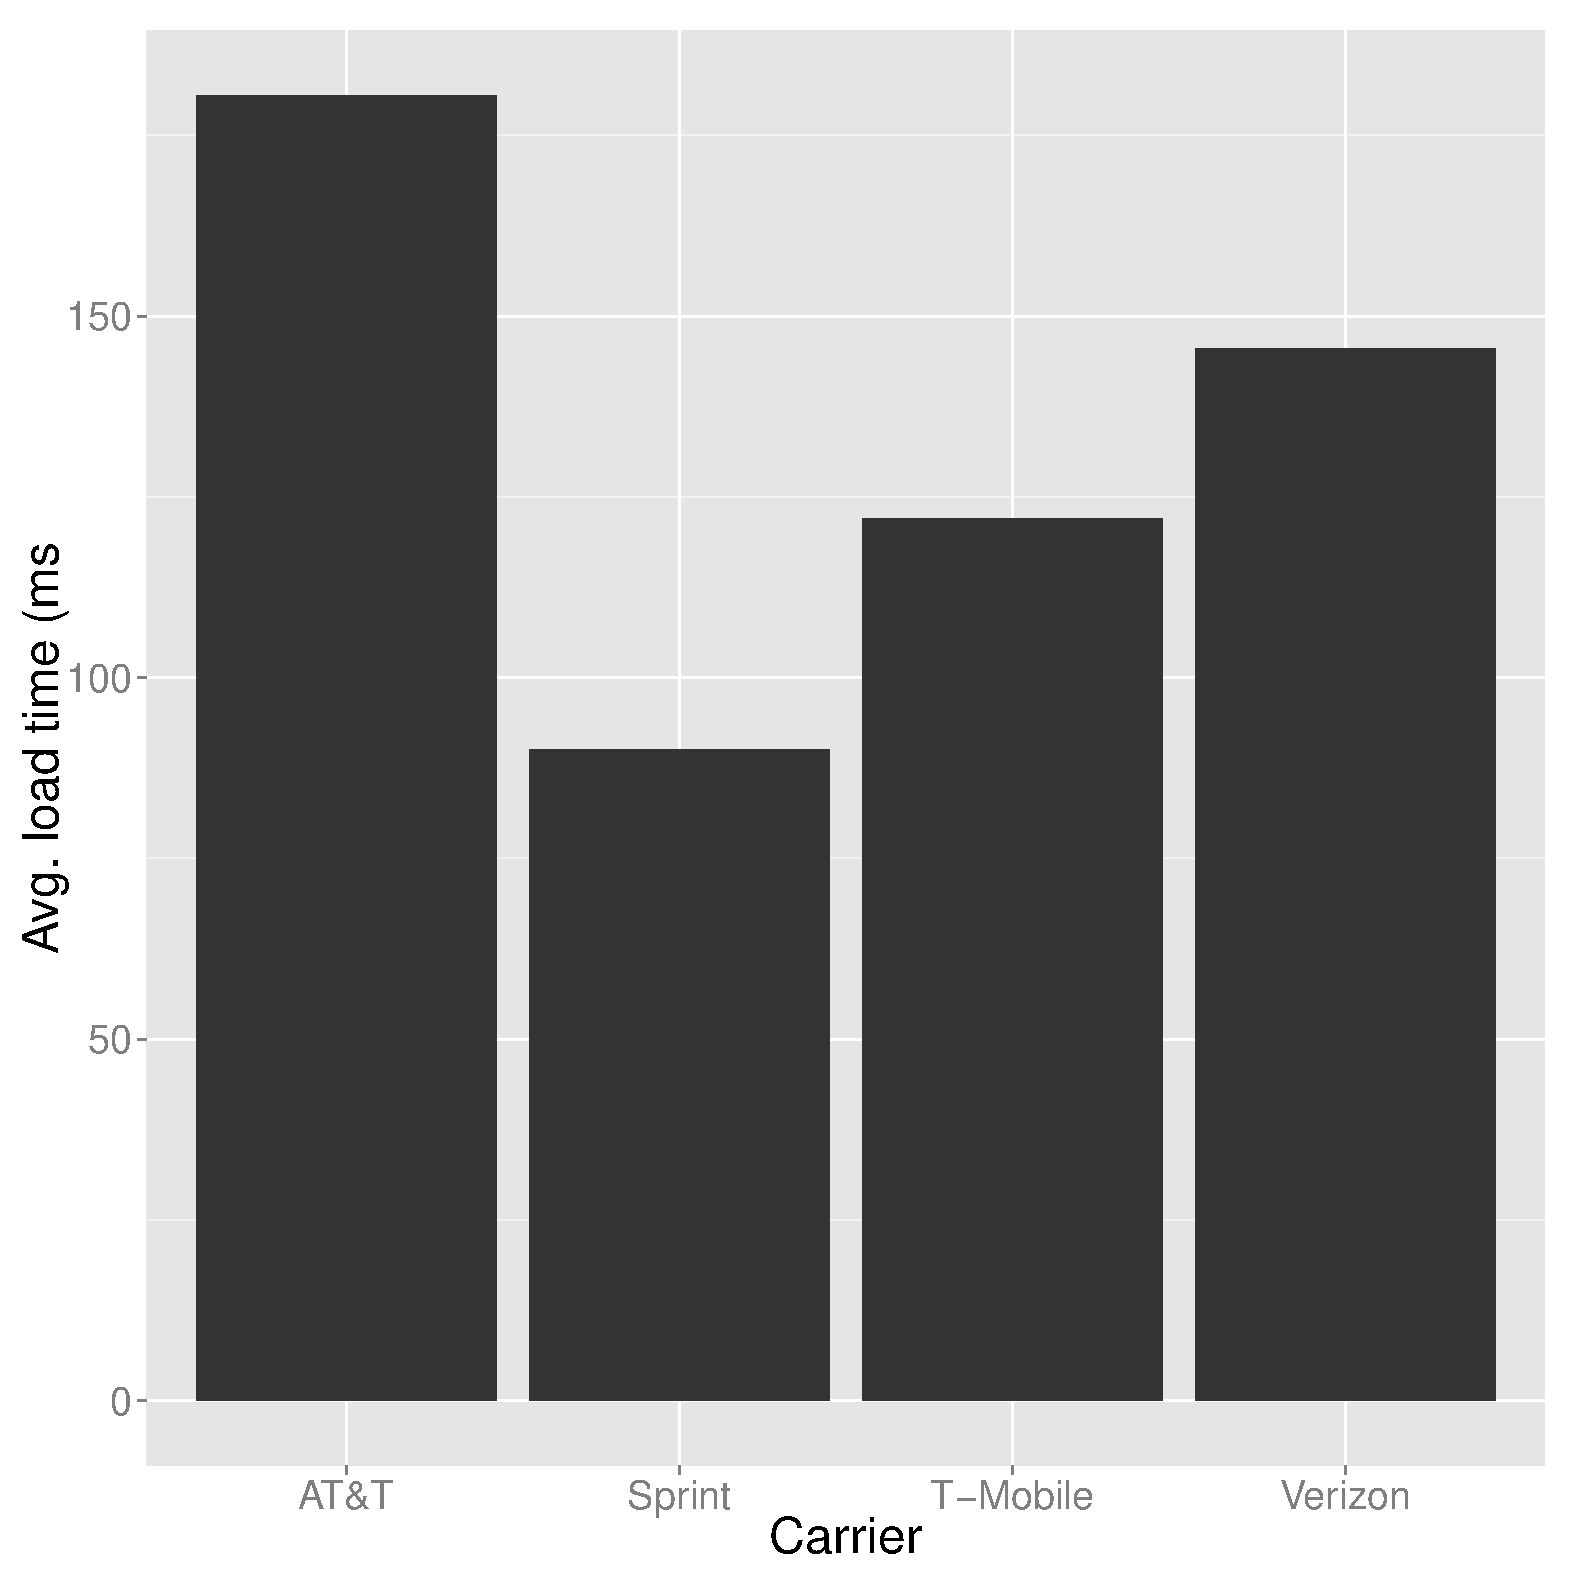
\includegraphics[width=4cm] {Images/dist1.pdf}}
% 		\caption{Visualization: Average \\ Load Times by Carrier
% 		 for BadApp}
% 		\label{fig:staplerX}
% 	\end{subfigure}
	
% 	\centering
% 	\begin{subfigure}{0.49\linewidth}
% 		{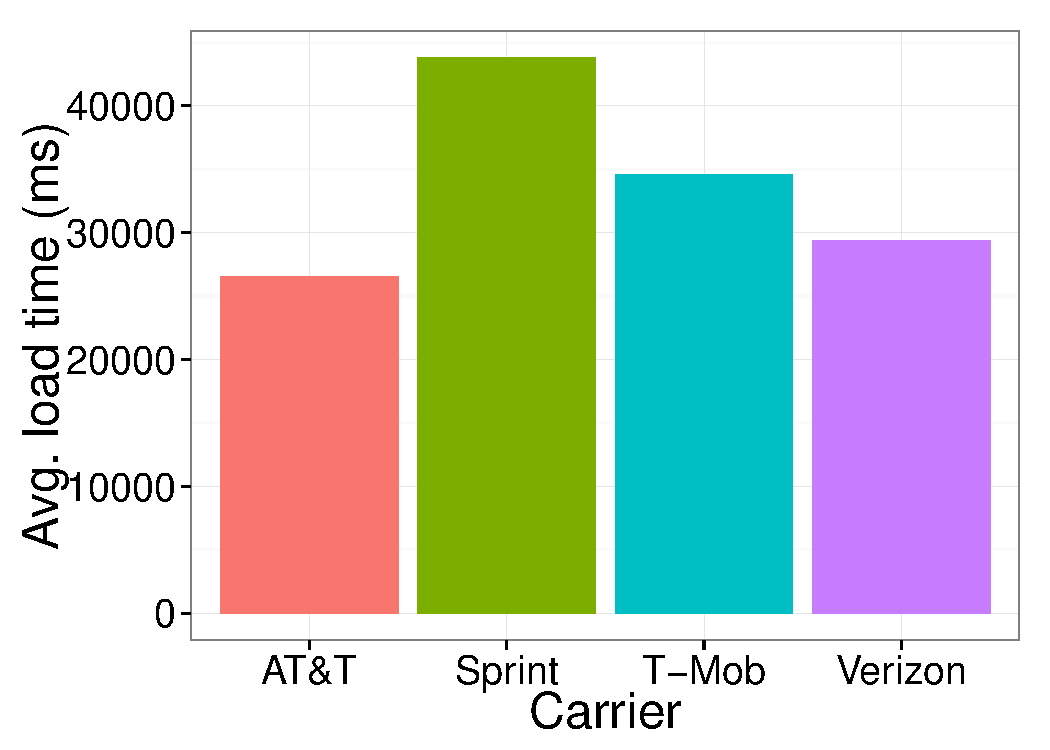
\includegraphics[width=4cm] {Images/dist2.pdf}}
% 		\caption{Scenario A: Average Load Times by Carrier}
% 		\label{fig:staplerX-a}
% 	\end{subfigure}
% 	\begin{subfigure}{0.49\linewidth}
% 		\centering
% 		{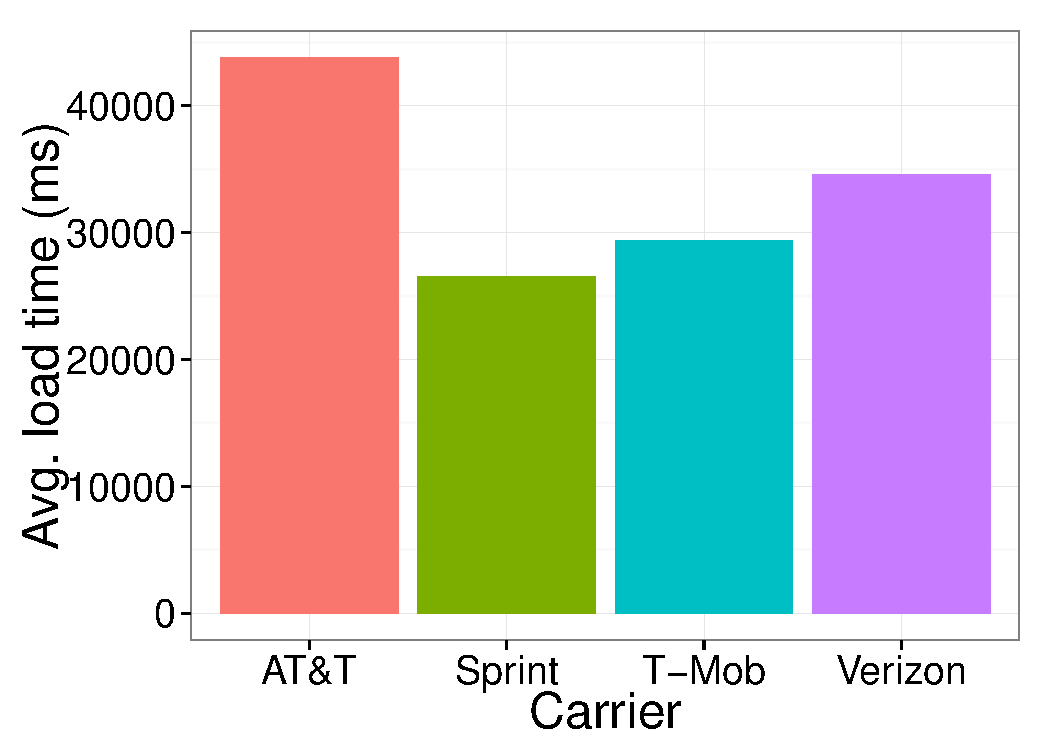
\includegraphics[width=4cm] {Images/dist3.pdf}}
% 		\caption{Scenario B: Average Load Times by Carrier}
% 		\label{fig:staplerX-b}
% 	\end{subfigure}
% 	\vspace{-10pt}
% 	\caption{Motivating Example}
% 	\label{fig:intro}
% 	\vspace{-15pt}
% \end{figure}

%%%%%% VLDB original end %%%%%%%

\reviewer {
	W2: Using the illustrative example is helpful, but would have been even more
helpful if it would be based on a real dataset actually used in the evaluations. 
Using the illustrative example was helpful and quite motivating.
However, this introduced another dataset not used in the evaluations
afterwards. To use a dataset, which was actually used in the evaluation would
make the presentation more coherent. Figure 1 uses the BadApp dataset,
Figure 3 a donation dataset, then other datasets are introduced for the
evaluation, and the diabetes dataset for the user studies. Focusing on the
diabetes dataset in Figure 1 and Figure 3 would leave more room to reuse
them to discuss some findings for example using Figure 3.
}
\mpv{sure, if we have time} \agp{I think this is worth investing 
the time in--shouldn't take more than half an hour to dig up, right? We can
also point at these visualizations and say that these were actually
returned by \SeeDB.}
\srm{I agree!}


\begin{example}
Consider a smartphone app analytics team that is tasked with answering why a certain app, 
BadApp, is showing poor performance and receiving consumer complaints. 
Suppose that the team uses the AppMetrics database containing metrics such as network usage, 
power consumption, and load times to perform the analysis.
The analyst begins by querying the AppMetrics database for BadApp-specific data and uses her 
favorite visualization software to graph various metrics for BadApp.

For instance, she may visualize average network usage for BadApp, 
correlation between session times and number of crashes, average load times by carrier, 
comparison of mobile operating systems running BadApp vs.~other apps, and so on,
in order to identify what metrics BadApp may be misbehaving on.
Depending on the types of visualizations created, the number of possible 
visualizations grows exponentially with the number of metrics in the database,
such that creating and examining all possible visualizations
becomes untenable.
% For example, the visualization for average load times by carrier is generated by running an operation equivalent to the
% SQL query (Q') shown below.
% %The result of this query is a two-column table that is very likely going to be viewed as a bar-char~\cite{vql, kristi}.
% Table \ref{tab:staplerX} and Figure \ref{fig:staplerX} respectively show an example of the results of Q' and a potential
% visualization.

% \noindent
% \begin{align*}
% & \tt Q' = SELECT \ \ carrier,\ AVG(load\_time) \ \ FROM \ \  AppMetrics \\
% & \tt \hspace{20pt} WHERE\ Name=``BadApp" \ \ GROUP  \ \ BY \ \ carrier
% \end{align*}



\begin{figure}[h]
\vspace{-10pt}
	\centering
	\begin{subfigure}{0.49\linewidth}
	   \begin{tabular}{cc} \hline
		  Carrier & Load Times (ms) \\ \hline
		  AT\&T & 180.55 \\ \hline
		  Sprint & 90.13 \\ \hline
		  T-Mobile & 122.00 \\ \hline
		  Verizon &  145.50\\ \hline
		  \end{tabular}
		  \caption{Data: Average Load Times by Carrier for BadApp} \label{tab:staplerX}
	\end{subfigure}
	\begin{subfigure}{0.49\linewidth}
		\centering
		{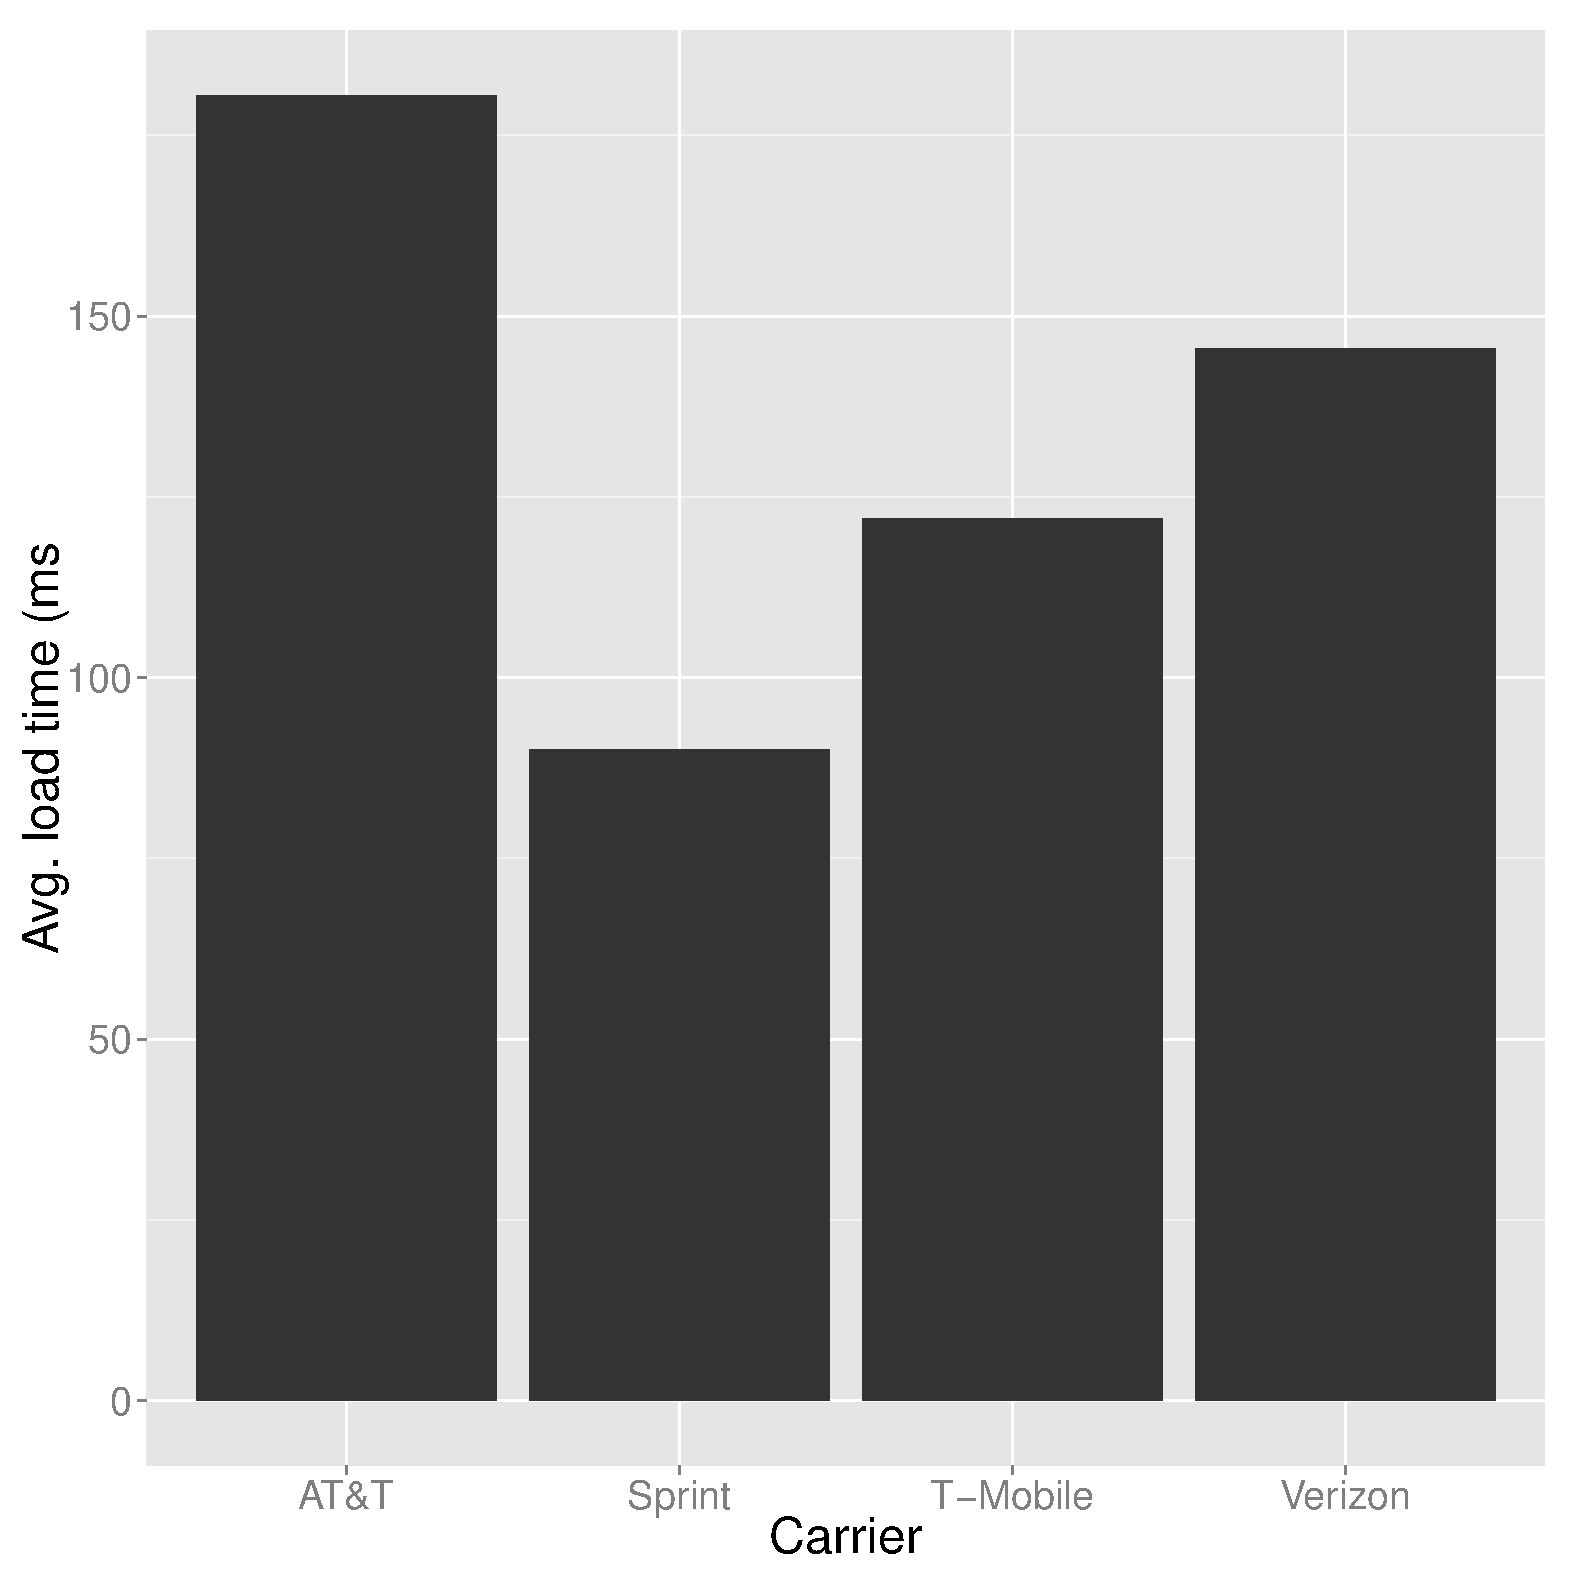
\includegraphics[width=4cm] {Images/dist1.pdf}}
		\caption{Visualization: Average \\ Load Times by Carrier
		 for BadApp}
		\label{fig:staplerX}
	\end{subfigure}
	
	\centering
	\begin{subfigure}{0.49\linewidth}
		{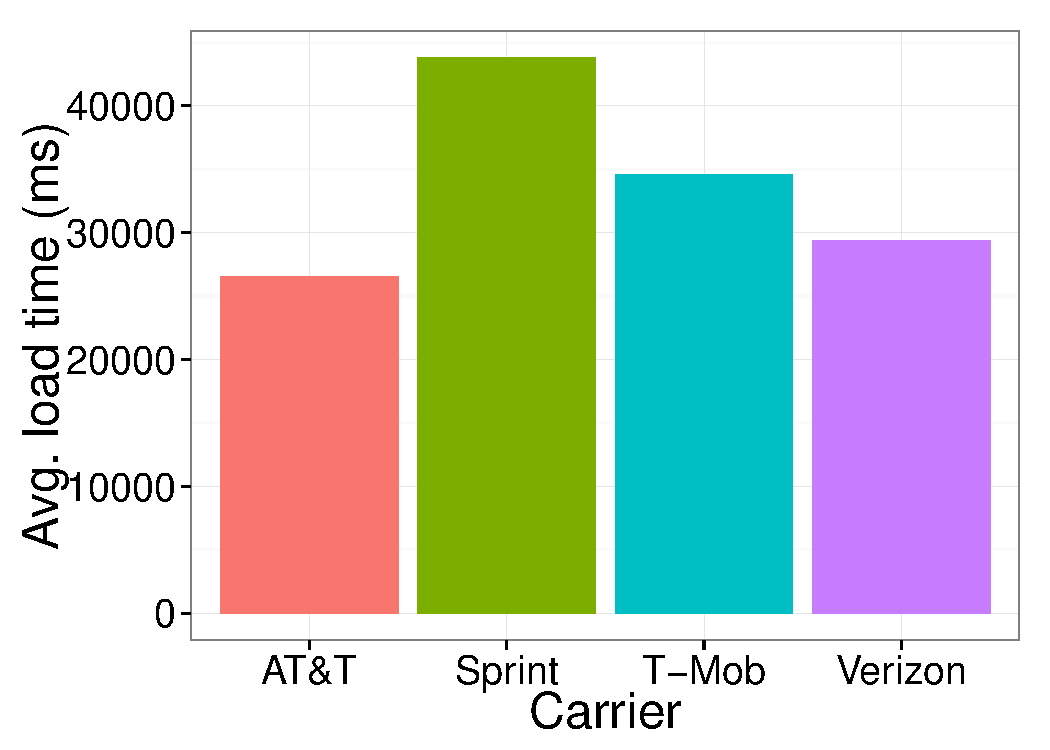
\includegraphics[width=4cm] {Images/dist2.pdf}}
		\caption{Scenario A: Average Load Times by Carrier}
		\label{fig:staplerX-a}
	\end{subfigure}
	\begin{subfigure}{0.49\linewidth}
		\centering
		{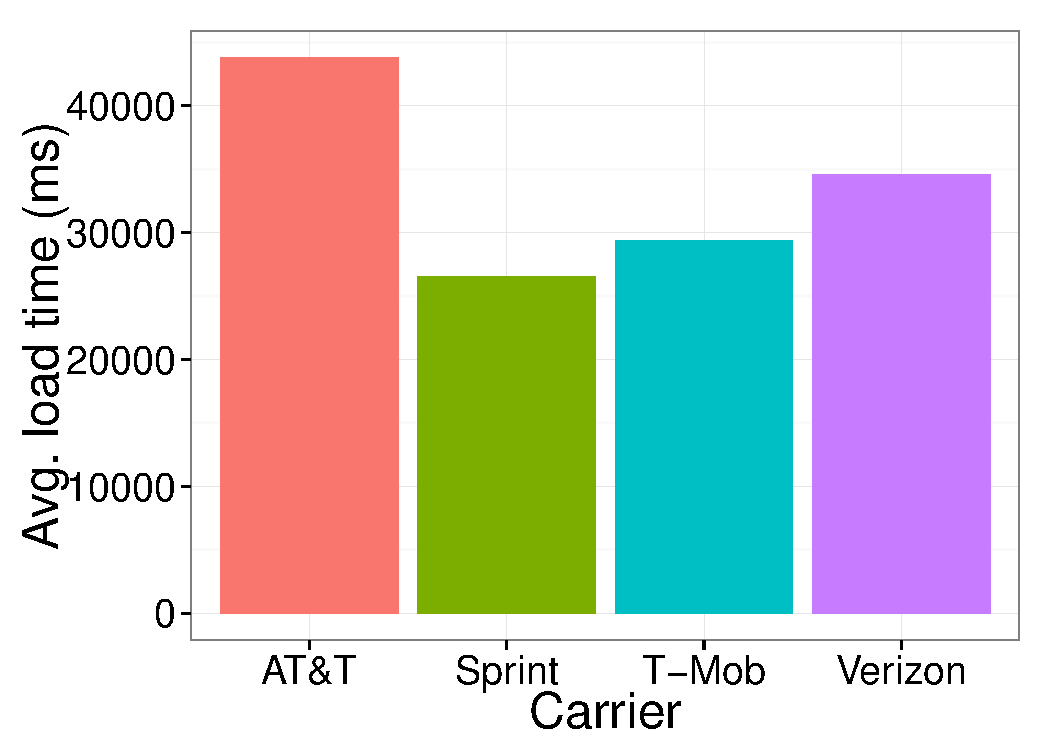
\includegraphics[width=4cm] {Images/dist3.pdf}}
		\caption{Scenario B: Average Load Times by Carrier}
		\label{fig:staplerX-b}
	\end{subfigure}
	\vspace{-10pt}
	\caption{Motivating Example}
	\label{fig:intro}
	\vspace{-15pt}
\end{figure}

%What might make one of these visualizations ``interesting'' or valuable for the 
%task at hand depends on a number of factors.
\srm{I suggested below that our user studies show that users like our metric. Do we believe this?}\agp{rewrote to remove preference}
As noted above, we have identified that 
analysts find visualizations that show
cases where the data deviates from some underlying distribution to be interesting.
In the case of app analytics, this underlying distribution might be metrics for
all apps, versus the distribution of particular metrics specifically in BadApp.
As an example, our user studies suggest that users will find the visualization of load times by carrier (Figure
\ref{fig:staplerX}) more interesting if the trend for load times across all
apps shows the {\it opposite} trend (e.g. Figure \ref{fig:staplerX-a}), and less interesting if the overall trend for all apps followed a similar trend.
(Figure \ref{fig:staplerX-b}).  
\end{example}



\mpv{acknowledge that this is from the vision paper?} \agp{Not necessary}

\mpv{Say that metric is suited to when there user is unfamiliar with the data, cold
starts?}
\agp{We need to articulate that our goal is to build \SeeDB that actually makes
these recommendations.}
%Since our goal with \SeeDB is to make visual analytics faster, we adopt a metric
%that prefers visualizations that show interesting or surprising trends in data.
%Specifically, we are motivated by the following observation:
%\begin{quotation}
%The greatest value of a picture is when it forces us to notice what we never expected to see.
%\end{quotation} 
%\begin{flushright} 
%- John Tukey, Exploratory Data Analysis 1977
%\end{flushright}

% While this utility metric is an example of a simple recommendation metric,
% it plays an important role in recommendations when 
% there is no prior history --- and therefore no user preferences
% or understanding of context.
% This special case is especially appropriate when the analyst
% is not very familiar with a dataset and is analyzing it for the first time.
% That said, in Section~\ref{sec:discussion}, we describe how our deviation-based
% metric can, in fact, encompass a large number of data-driven utility metrics and
% can be seamlessly extended to support other dimensions such as user preferences.

\srm{the following is substantially edited / cut back.}
We formally define the deviation-based scoring function in the next
section.  As noted above, in addition to our deviation-based metric,
there are of course many other dimensions (aesthetics, user
preferences, etc.) that can influence the perceived utility of a
visualization a few of which we discuss in Section
\ref{sec:discussion}, leaving a detailed investigation of such metrics
for future work.


%These include other functions based on data distribution (e.g. scoring based on 
%statistical summaries) and functions that measure utility along {\em 
%dimensions} other than data distribution. 
%These utility dimensions 
%include aesthetics (e.g. is a bar plot more appropriate than a 
%scatter plot), context (e.g. prior knowledge that only female patients visit the
%obstetrics department), and user preference (e.g. in the sales dataset, profit is
%the most relevant attribute).
%Exploration of each of these dimensions forms a distinct body of work.

% functions 
% that can be used to score the utility of a 
% visualization; these can be different functions based on data distribution (e.g. scoring
% based on statistical summaries of data or outlier detection) or functions that take
% orthogonal {\em dimensions} of utility into account, e.g., user preferences, aesthetics, and context.
% The pruning framework we propose in Section \ref{sec:in_memory_execution_engine} can be applied to a large set of 
% functions derived from data distribution, and \SeeDB
% can support these metrics without any changes. \mpv{Verify true? Add characterization
% of metrics}
% Investigations of the other dimensions of utility form a distinct body of work, and
% we leave these explorations for future work.
% \mpv{keep? In section \ref{sec:discission}, we outline some means by which \SeeDB may be 
% extended to support these metrics.}
% We leave the investigation of other dimensions of utility to future work, but outline
% in Section \ref{sec:discussion} some means by which \SeeDB may be extended to support them.

% Due to the scale of data, most common visualizations show aggregate summaries of data
% as opposed to individual records (e.g. average sales by state vs. sales of each store 
% in every state).
% Consequently, our current implementation of \SeeDB\ recommends visualizations that show aggregate 
% summaries of data.

% Of course, there are a variety of other possible data-driven metrics for quality or utility
% of a visualization.
% For instance, one might focus on visualizations that show order statistics or anomalies~\cite{DBLP:conf/avi/KandelPPHH12}. 
% These would be important for spotting, for example, unusual spikes in machine load.
% Similarly, drawing upon the literature on data cubes, one might choose visualizations that highlight aggregates that
% are unusual given the remaining values in the cube~\cite{DBLP:conf/vldb/Sarawagi00}.
% Finally, one might choose to not aggregate any values but show correlations between attributes by plotting a random
% sampling of data-points.  Incorporating these other types of visualizations into our framework is an interesting
% direction for future work.

\reviewer{
	The method does not consider the context, semantics, and any user
preferences all important components of viz	
}
\mpv{Yeah I say that above. Any additions?}



% The majority of visualizations that are generated in visualization systems are based on aggregate summaries of the
% underlying data.
% As a result, the {\it trends} we study are the results of grouping and aggregation applied to a given dataset.


% Thus, the recommendation algorithm used by \SeeDB\ works as follows: given a dataset $D$ and a query $Q$
% indicating the subset of data of interest to the analyst, \SeeDB finds the visualizations of $Q$ that 
% show the highest deviation between trends in $Q$ and trends in $D$. 
% Specifically, \SeeDB considers visualizations that can be constructed via a combinations of grouping and 
% aggregation applied to $Q$.

No existing system is that we are aware of makes use of variation in the underlying
data to recommend visualizations.  
Current visualization packages like Spotfire~\cite{Ahlberg:1996:SIE:245882.245893} and Tableau~\cite{tableau,polaris} have limited capabilities for 
recommending visualizations.
Their recommendations only implement rules-of-thumb 
regarding chart aesthetics such as choice of
chart type, colors and marks, borrowed from
classical work by Mackinlay~\cite{Mackinlay:1986:ADG:22949.22950} and Cleveland and Gill~\cite{cleveland1984graphical}.
%No existing system that we are aware of leverages insights about the underlying data
%into make visualization recommendations. \mpv{does this sound ok?} \agp{I would start with
%the statement that no current system supports the recommending of interesting visualizations
%where the target dataset shows some discrepancies not found in the underlying data.
%Then say the first two lines.}


Our system, \SeeDB, is built as a middleware layer that can run on any 
relational database system (row or column store), 
seamlessly benefiting from optimizations to 
the database. 
In this paper, we develop and validate the use of  
two orthogonal techniques to make tractable the problem
of recommending visualizations based on deviation:
\begin{denselist}
\item {\em Sharing Computation.} 
We develop a suite of multi-query optimization techniques to share computation
among the candidate visualizations,
reducing time taken by ?X. \agp{fill in.}
\item {\em Pruning Computation.}
We develop a pruning technique to avoid wasting computation
on obviously low-utility visualizations, adapting
techniques from traditional 
  confidence-interval-based~\cite{hoeffding1963probability} 
  top-$k$ ranking and the
  multi-armed bandit~\cite{bandits},
  further reducing time taken by ?X. \agp{fill in.}
\end{denselist}
Lastly, we develop a general {\em phase-based execution framework}
that allows us to leverage the benefits of these two techniques
in tandem, reducing the time for execution by over ?X,
making recommendations feasible in real-time. \agp{fill in}

We present the experimental evaluation of \SeeDB 
via both a performance study and a user study.
In summary, the contributions of this paper are:

% efficiently manages the search
% for data-driven visualization recommendations at interactive time scales.
% We show that \SeeDB can be implemented on top of a traditional relational database,
% allowing it to take advantage of the benefits of the interfaces and features
% relation engines expose.
% Doing this, however,
% also leads to inefficiencies that arise due to the requirement that data be
% accessed via SQL.   
% We manage these inefficiencies by introducing two classes of optimizations:
% {\em sharing-based} optimizations, that try to batch
% and share as much computation as possible to minimize the number of SQL queries,
% and {\em pruning-based optimizations}, that try to avoid
% as much unnecessary work as possible, and discarding candidate aggregate views
% that are of low utility.

\mpv{revisit contributions} \agp{The order of this is off.}
\begin{denselist}
%  \item We design \SeeDB as a system for data-driven visualization recommendations.
%  We explore and evaluate two distinct implementations of the system, one as a
%  wrapper around a database and another a custom solution (Section~\ref{sec:system_architecture}).
  \item We present \SeeDB, a visualization recommendation system that can run
  as a middleware layer on any SQL-compliant DBMS (Section~\ref{sec:system_architecture}).
  \item We adopt and evaluate a deviation-based scoring function for measuring utility
  of a visualization (Section~\ref{sec:problem_statement}).
  \item We propose a set of multi-query optimization techniques which in combination
  with the pruning framework maximize the sharing of computation between visualization
  computations (Section~\ref{sec:sharing_opt}).
  \item We propose a general-purpose view pruning framework to quickly identify
  high-utility visualizations by adapting techniques from traditional 
  confidence-interval-based~\cite{hoeffding1963probability} top-$k$ ranking and the
   multi-armed bandit problem~\cite{bandits} (Section~\ref{sec:in_memory_execution_engine}).
  % \item We describe a general deviation-based framework 
  % for evaluating the utility  of a visualization,
  % and present and evaluate a specific metric that identifies 
  % aggregate dimensions in a dataset that
  % show maximal variation (Section~\ref{sec:problem_statement}).
  % We develop two classes of optimizations to make such aggregates run fast 
  % in a conventional DBMS.
  % \item The first set of techniques
  % combine queries and aggregates to minimize the number of queries executed and 
  % maximize the sharing of scans between queries, 
  % including bin-packing~\cite{garey} algorithms and parallelization
  % (Section~\ref{sec:sharing_opt}).
  % \item The second set of techniques further optimize the process by adapting techniques 
  % from both traditional confidence-interval-based~\cite{hoeffding1963probability} top-$k$ ranking and the
  %  multi-armed bandit problem~\cite{bandits} 
  %  to the problem finding the top-$k$ visualizations (Section~\ref{sec:in_memory_execution_engine}).
  % \item We explore visualization pruning techniques based on data distribution
  % to prune visualizations even before they are evaluated by the \SeeDB\ system 
  % (Section~\ref{sec:pruning}).
  \item We evaluate the performance of our pruning framework and demonstrate that \SeeDB
  can identify high-utility visualizations with high accuracy. We also demonstrate that 
  our optimizations provide a 40-100X speedup on both relational row and column stores
  (Section~\ref{sec:experiments}). 
  \item We present the results of a user study evaluating the role of visualization 
  recommendations in visual analysis and the quality of \SeeDB recommendations in particular
  (Section \ref{sec:user_study}), showing that our deviation-based metric is able to yield visualizations that users find interesting.
\end{denselist}

\noindent Finally we note that the vision for \SeeDB\ was described in a vision paper~\cite{DBLP:conf/vldb/Parameswaran2013} and presented as demonstration~\cite{DBLP:journals/pvldb/VartakMPP14}, but neither of these short papers described detailed algorithms or
presented any form of evaluation.
Specifically, this work builds upon the \SeeDB vision by proposing a novel, general-purpose view 
pruning framework, a combination of multi-query optimization techniques, and presenting 
both a performance study of the system as well as a user study demonstrating the efficacy of our system in aiding analysis.
\reviewer{
	I like the ideas in this paper, but they have been presented in a vision paper
and demo paper. So to warrant a new publication the execution of these
ideas (the specific search techniques) and their evaluation need to be novel,
interesting, and well executed. I found the evaluation in particular to be
lacking.
}

\reviewer{
	This paper’s contribution seems to be mostly section 4.3 (pruning
optimizations) and the tests (Sections 5 and 6). The differences with
references [27] and [37] should be made more clear.
}



 %!TEX root=document.tex
\section{Problem Statement}
\label{sec:problem_statement}
\resolved{
\srm{This rewrite is good, thanks Aditya!}
\srm{We need to define what measure and dimension attributes mean;
in a snowflake schema a dimension attribute would be anything in a dimension table, and a measure attribute would be a non-foreign
key column in a fact table. I don't think that's what we mean.  I think these are actually properties of the query, right, i.e., 
dimension attributes are those appearing in the group by clause?  We should use different names.}\agp{I've addressed this somewhat.}
}
As is standard in OLAP, and in visual analytics
tools such as Tableau and Polaris~\cite{tableau,polaris},
we focus on a database $D$ with a snowflake schema.
We denote the attributes
that we would like to group-by in our visualizations 
as {\em dimension attributes}, $A$, and 
the attributes that we would like to 
aggregate in our visualizations
as {\em measure attributes}, $M$.
Further, we denote by $F$ the set of potential
aggregate functions over the measure attributes (e.g. COUNT, SUM, AVG).  
For visualization purposes, we assume that we can group $D$ along any of the dimension attributes $A$ 
and we can aggregate any of the measure attributes $M$.
This leads to a two-column table that can be easily visualized
via standard visualization mechanisms, such as bar charts or trend lines.
(Recent work has shown that bar charts are the overwhelming majority of visualizations
created using visual analytics tools~\cite{DBLP:journals/pvldb/MortonBGM14}.) 
Our techniques also apply to the general Polaris table algebra~\cite{polaris}, where
we can aggregate across multiple attributes at once, and group-by multiple attributes, 
potentially leading to more than two columns.
For ease of exposition, we focus on two-column result visualizations in this paper,
which can be readily visualized using bar charts or trend lines.

In addition to the database $D$, we assume that the analyst has indicated
a desire to explore a subset of data specified by a query $Q$.
The goal of \SeeDB is to recommend visualizations of $Q$ that have
high utility (which we measure using deviation, as explained below).
The class of queries $Q$ posed over $D$ that we support encompass a general class of queries 
that select a horizontal fragment of the fact table and one or more dimension tables.
Conceptually, we can view this as a simple selection query over the result of joining all
the tables involved in the snowflake schema. 
That said, we can also support projections and joins which essentially have the effect
of respectively dropping certain columns or tables from consideration in the visualizations.
Thus, we support a general class of select-project-join (SPJ) queries over the snowflake schema.
For the purpose of this discussion, we focus on simple selection
queries over the result of joining all the tables in the snowflake schema.
We note that this class of queries 
suffices for most visualization tasks.
For instance, in our illustrative example, $Q$ can select any subset of records from the
Census table. 
We denote the result of $Q$ as $D_Q$.
\resolved{
\srm{Although this notion is compact, it doesn't seem to capture
the contents of the WHERE clause.}\agp{rewritten to make clear that
it is a function.}
}

Each \SeeDB visualization  can be translated into an agg\-re\-gate / group-by
 query on the underlying data.
% Since each visualization represents an aggregate summary of the underlying data,
% the visualization can be distilled into an aggregate and grouping query.
% Borrowing from the data cube literature~\cite{olap}, 
% we call these summaries aggregate {\it views}.
% where an aggregate view
% is the result of applying grouping and aggregation to a dataset.
We represent a visualization $V_i$ 
 as a function represented by a triple $(a, m, f)$, 
where $m \in M, a \in A, f \in F$.   
We call this an {\em aggregate view} or simply a {\em view}.
The aggregate view performs a group-by on $a$ and applies the aggregation function $f$ 
to measure attribute $m$. 
As an example, $V_i(D)$ represents the results of grouping
the data in $D$ by $a$, and then aggregating the $m$ values using $f$;
$V_i(D_Q)$ represents a similar visualization applied to
the data in $D_Q$.
% While \SeeDB techniques can be used to recommend visualizations
% generated via multi-attribute grouping and aggregation,
% for simplicity, we focus on views generated by single attribute grouping. 
\resolved{
\reviewer {D1.2 I wonder what is really specific to visualizations. Indeed, a visualization
as defined by the authors seems to be a two column table (attribute,
measure). Is it usual to define visualizations this way?
}
\mpv{
	Aggregate summaries visualized as bar charts and column charts are in fact, extremely
	common visualizations, and hence are the first visualizations tackled by \SeeDB.
	The techniques we develop here are general and have possible applications 
	in traditional data mining. It would be interesting to explore these applications
	further.
}
\agp{I think we can amend the response to say it is standard (cite polaris table algebra)
to define visualizations in this manner.}
}
\if{0}
Given a database $D$ and the subset of data selected by the analyst (via query $Q$), 
the goal of \SeeDB is to recommend visualizations of $Q$ that have high utility. 
\SeeDB (currently) focuses on recommending bar charts showing aggregate views of the 
data.
This choice is motivated by the fact that bar plots are the overwhelming
majority of visualizations created using visualization tools 
\cite{DBLP:journals/sigmod_record/MortonBGKM14}.
\fi
% The most common visualizations in real workloads of Tableau and ManyEyes 
% are bar charts \cite{DBLP:journals/sigmod_record/MortonBGKM14} showing aggregate views
% of the data. 
% Furthermore, the scale of data necessitates the visualization of aggregate summaries of
% data vs. individual records (e.g. average sales by state vs. sales of each store in the
% country).
% Consequently, \SeeDB (currently) focuses on this specific type of visualization.
% Due to the scale of data, most common visualizations show aggregate summaries of data
% as opposed to individual records (e.g. average sales by state vs. sales of each store 
% in every state).
% Moreover, these summaries are visualized as bar charts and column charts in the vast
% majority of cases~\cite{kristi}.
% Consequently, our current implementation of \SeeDB focuses on recommending bar and column
% charts that visualize aggregate summaries.
% Given a database $D$, associated schema $S$, and a user query $Q$, the goal
% of \SeeDB\ is to recommend visualizations of results of $Q$ with high utility. 
% As mentioned in Section~\ref{sec:introduction}, \SeeDB\ focuses on visualizations 
% that show aggregate summaries of data.
\if{0}
Let $D$ have a snowflake schema with 
dimension attributes $A$, measure attributes $M$, and potential
aggregate functions $F$ over the measure attributes. 
%Similar to cube aggregates, 
For visualization purposes, we assume that we can group $D$ along any of the dimension attributes $A$ 
and we can aggregate any of the measure attributes $M$.
Our system currently limits the class of queries $Q$ posed over $D$ to be single-table
selection (and optionally projection) queries.
We find that simple selection queries suffice for most visualization tasks.
For instance, in our illustrative example, $Q$ can select any subset of records from the
AppMetrics table. 
Adding projections to $Q$ serves to limit the the dimension and measure 
attributes used by \SeeDB in constructing visualizations.
We denote the result of $Q$ as $D_Q$.
\fi
% dimension attributes are either nominal, ordinal, or numeric,
% but typically with a small number of distinct values;
% these are the attributes along which we can perform a group-by.
% Measure attributes are numeric attributes which take on a large number 
% of distinct values; 
% these are the ones that are typically aggregated.
% We limit the class of queries $Q$ posed over $D$ to be
% those that select one or more rows from the fact table, 
% and denote the results as $D_Q$. 
% For instance, in a product sales table, $Q$ could select
% all tuples corresponding to transactions involving bicycles.
% Given query $Q$, \SeeDB\ considers all aggregate views 
% $V_i$ obtained by performing a grouping and aggregation on $D_Q$. 
\resolved{
\reviewer{The range of queries that are supported is not clear. Specially in fig.3, in
the ``SQL'' tab, it seems that users can only define very simple selection
queries (where the selection is a simple conjunction of predicates). No
project, no joins, no difference, no grouping/agg. Is this correct? Why call
this SQL?}
\mpv{New interface only allows selections}
\agp{I don't think we should restrict ourselves to selection. We can
support SPJ queries over the snowflake schema.}
}
\resolved{
\reviewer {
	D2.1 The approach seems limited to simple queries of the form Select * from
aTable where someSelectionPredicates. It seems to me that it is quite a
limitation in the sense that the authors implicitly position their work in a data
warehouse exploration context (as per Section 2). I would like the authors to
comment that point. For instance, what about when the projection is not
select * but select aListOfAttributes?
}
\mpv{Do we need to defend why we support only simple queries? From other studies of
visualization tools, a significant portion of queries posed in these tools is 
limited to simple selection and projection tasks ~\cite{}.
Therefore, we have prioritized support for operations over more complex queries.}
\agp{I think we can clarify this in the response, but see what I've said above.}
}
\resolved{
\reviewer {
	D2.2 In the definition of $U(V_i)$: as $D_Q $contains a selection that D does not
have, how to ensure that the population of the two distribution is the same?
}
\mpv{
	This should only be in the reviewer response: the dataset under study $D_Q$ can be
	compared to various {\em comparison} datasets; by default, the comparison dataset
	is set to the full dataset $D$ (to observe overall trends), but can be set to any 
	other subset of data.
	Depending on the analytical task, one may want the two populations to be similar 
	(males and females in a given age group) or different (comparison of young adults to seniors). 
	Since the system has limited knowedlge about the exact analytical task, we provide 
	users with flexiblity to choose a comparison dataset.
}
}
% Note that all such $V_i$ give rise to two-column results that can 
% be readily visualized (e.g. Table~\ref{tab:staplerX}). 
% Consider a database $D$, and associated metadata $M(D)$, with a snowflake schema,
% with dimension attributes $A$, measure attributes $M$, and potential
% aggregate functions $F$ over the measure attributes.
% Dimension attributes are either nominal, ordinal, or numeric,
% but typically with a small number of distinct values;
% these are the attributes along which we can perform a group-by.
% Measure attributes are numeric attributes which take on a large number 
% of distinct values; 
% these are the ones that are typically aggregated.

% Given a database $D$ and a query $Q$, \SeeDB\ considers a number of views (i.e., aggregate queries) that
% can be generated from $Q$ by adding relational operators.
% For the purposes of this discussion, we will refer to views and visualizations
% interchangeably, since it is straightforward to translate views into
% visualizations automatically~\cite{DBLP:journals/cacm/StolteTH08}. 
% For example, there are straightforward rules that
% dictate how the view in Table~\ref{tab:staplerX} can be transformed to give a
% visualization like Figure~\ref{fig:staplerX}.

% For this work, we classify attributes of a table into
% two types: {\it dimension attributes} and {\it measure attributes}. 
% Dimension
% attributes are attributes that are nominal, ordinal or numeric but with a small
% number of distinct values. 
% These are the attributes along which we can perform a group-by. 
% Measure attributes on the other hand are numeric attributes will a
% large number of distinct values. 
% We consider views where the dimension attributes are
% aggregated with respect to these measure attributes.
%Lastly, for simplicity, 
%we ignore {\em binning}: that is, given a view to be visualized,
%there are many ways of binning values to give the view. 
%For instance, if we have average profits per day, we can bin the days into
%months, into weeks, or into years.
%  aggregate view $V_i$ by
% comparing data distribution in the query results to the data distribution of the underlying dataset.
% taking into consideration a variety of aspects, including
% user preferences, metadata, query data, background data, and context.
% For now, and for most of the paper, however, 
% That said, our techniques also seamlessly apply to a more general 
% class of distance metrics described in .
\SeeDB determines the utility of 
visualizations via deviation; visualizations that show different trends in the query
dataset (i.e. $D_Q$) compared to a reference dataset (called $D_R$) are said to have high
utility.
The reference dataset $D_R$ may be defined as the entire underlying dataset ($D$),
the complement of $D_Q$ ($D$ - $D_Q$) or data selected by any arbitrary query $Q'$ ($D_{Q'}$).
The analyst has the option of specifying $D_R$; we use $D_R = D$ as the default if the analyst does not specify a reference. 
% We discuss in Section~\ref{sec:other_utility_metrics} how other distance metrics can be 
% incorporated into our system without any changes. 
Given a view $V_i$, the deviation-based utility of $V_i$ is
computed as the deviation between the results of applying $V_i$ to the query data, $D_Q$,
and applying $V_i$ to the reference data, $D_R$.
View $V_i$ applied to the results of $Q$ can be expressed as query $Q_T$ below. 
We call this the {\em target view}.
$$ Q_T\ =\ {\tt SELECT \ } a, f(m) \ \ {\tt FROM} \  D_Q\  {\tt GROUP \ \ BY} \ a$$ 
Similarly, view $V_i$ applied to the reference data $V_i (D_R)$ can be expressed as $Q_R$. 
We call this the {\em reference view}. 
$$ Q_R\ =\ {\tt SELECT \ } a, f(m) \ \ {\tt FROM} \  D_R\  {\tt GROUP \ \ BY} \ a$$
The (two) SQL queries corresponding to each view are referred to as {\em view queries}.
The results of the above view queries are summaries with two columns, namely $a$ and
$f(m)$. 
To ensure that all aggregate summaries have the same scale, we normalize each 
summary into a probability distribution (i.e. the values of $f(m)$ sum to $1$).
% over the various values of $a$ and the tables can be normalized into
%probability distributions for comparison. To convert each result table 
For our example visualization of {\em Average Capital Gain vs. Sex} (Figure \ref{fig:intro}),
the probability distribution for the target view $V_i(D_Q)$ ({\em unmarried} adults), 
denoted as $P[V_i (D_Q)]$ is: 
(F: 0.52, M: 0.48) while that for the reference view $V_i(D_R)$ ({\em married} adults), 
denoted as $P[V_i (D_R)]$ is:
(F: 0.31, M: 0.69). 
In contrast, the distributions for the visualization {\em Average Age
vs. Sex} are (F: 0.5, M: 0.5) and (F: 0.51, M: 0.49) 
for the target and reference view respectively.
Qualitatively, we see that the distributions show a large deviation for
the former visualization and hardly any deviation for the latter.

Given an aggregate view $V_i$ and probability distributions for the
target view  ($P[V_i (D_Q)]$) and reference view ($P[V_i (D_R)]$), we
define the {\em utility} of $V_i$ as the distance between these two probability
distributions. The higher the distance between the two distributions, the more 
likely the
visualization is to be interesting and therefore higher the utility.
Formally, if $S$ is a distance function,
$$ U (V_i) = S ( P[V_i (D_Q)], P[V_i (D_R)] )$$
% The utility of a view is our measure for whether the target view is
% ``potentially interesting'' as compared to the comparison view:
% the higher the utility, the more the deviation
% from the comparison view, and the more likely the associated visualization is to be interesting.
Computing distance between probability distributions has
been well studied in the literature, and \SeeDB\ supports a variety of distance
functions
to compute utility, including Earth Movers Distance, 
Euclidean Distance, Kullback-Leibler Divergence (K-L
divergence), and Jenson-Shannon
Distance. 
Our experiments use Earth Movers Distance as the default distance function,
but in Section \ref{sec:discussion} we discuss results for
other distance functions. 
Also in Section~\ref{sec:discussion}, we describe how our utility metric
can be generalized to capture other aspects of interest to analysts (beyond deviation).

We can formally state the \SeeDB problem as follows:
% Computing distance between probability distributions has
% been well studied, and \SeeDB\ supports a variety of metrics including
% to compute this distance.

% The metric may be supplied by the user, with their
% application in mind.
% Our current prototypes have the following in-built metrics
% to compute utility:
% \begin{denselist}
%   \item {\bf Earth Movers Distance (EMD)}~\cite{wikipedia-prob-dist}: Commonly used to
%   measure differences between color histograms from images, EMD is a popular metric for comparing
%   discrete distributions. This is the default metric used in \SeeDB.
%   \item {\bf Euclidean Distance}: The L2 norm or
%   Euclidean distance considers the two distributions to be points in a high
%   dimensional space and measures the distance between them.
%   \item {\bf Kullback-Leibler Divergence}(K-L divergence)~\cite{wikipedia-KL}:
%   K-L divergence measures the information lost when one probability distribution is used to approximate
%   the other one.
%   \item {\bf Jenson-Shannon Distance}~\cite{wikipedia-JS,entropy-vis}: Based on
%   the K-L divergence, this distance measures the similarity between two probability distributions.
% \end{denselist}
% Finally, we note that while other definitions of the comparison views and
% utility metrics are possible, for our initial exploration into 
% visualization recommendations, we chose to focus on the intuitive definitions above.
% In Appendix~\ref{sec:example-viz}, we perform a qualitative study of the EMD
% metric showing that it returns interesting results on real-world datasets.
% \mpv{Choice of metric should have been explained by this point}

% While we set the default \SeeDB\ distance metric as EMD (due to its simplicity),
% users can choose to use any of the distance metrics defined above. We note that
% the above definition of a view and its utility is merely one of many possible
% definitions and we choose this particular definition for simplicity and its
% intuitive nature. 
\begin{problem}
\vspace{-5pt}
Given a user-specified query $Q$ on a database $D$, a reference dataset $D_R$, 
a utility function $U$ as defined
above, and a positive integer $k$, find $k$ aggregate views $V \equiv (a, m, f)$ that
have the largest values of $U(V)$ among all the views $(a, m, f)$, 
while minimizing total computation time.
\vspace{-5pt}
\end{problem}
% Thus, \SeeDB\ aims to find the $k$ views (obtained by adding a single aggregate
% and group-by operator) that have the largest utility based on the function $U$.

% While the problem definition above assumes that we have been provided with a
% query $Q$ and we compare views on $Q$ with corresponding views on the entire
% database $D$, the \SeeDB\ framework is agnostic to where the comparison
% dataset is coming from and its contents. So the same formulation works for Use
% Cases II and III discussed in Section \ref{sec:introduction}. 





%Trend in the subset of the data that deviates from the corresponding trend in
%the overall data.
 %!TEX root=document.tex

\section{{\large \SeeDB} Front-End \& Architecture}
\label{sec:system_architecture}

%In this section, we present an overview of the \SeeDB\ architecture.
% Given an input query on a dataset, the goal of \SeeDB is to recommend
% visualizations the analyst would find most valuable.
% \SeeDB recommends visualizations that the analyst would find most valuable,
% taking into account aspects such as the background, user preferences,
% and context (as discussed in Section~\ref{sec:general-metric}).

We now describe \SeeDB's front-end user experience, and then
describe the architecture and the execution engine in more detail.

\stitle{Front-end Experience.} 
We packaged \SeeDB as a recommendation plugin that can
be incorporated into a visualization tool such as Tableau or Spotfire. 
For evaluating our system, we have combined \SeeDB with a simple visualization
builder interface inspired by Polaris~\cite{polaris}.
Figure~\ref{fig:frontend1} shows the web front-end for \SeeDB 
comprising four parts 
(A) dataset selector used to connect to a database and query a specific collection of tables; 
(B) query builder used to
formulate queries using a form-based interface; 
(C) visualization builder used to manually specify visualizations; and 
(D) \SeeDB recommendations plugin 
that displays recommended visualizations.
The recommendations provided by \SeeDB change in 
response to changes in the query (B)
issued against the database.
\resolved{\srm{This is the first mention of ``human in the loop'' philosophy.  I think it might be good
to promote this to an earlier part of the paper, but only if we feel like we have something interesting
to say about it.}}
%SRM cut this -- we already said it and it doesn't really matter to VLDB reviewers
%Note that supporting basic visualization specification 
%capabilities a la Polaris, coupled with automated recommendations enabling
%the reduction of tedious manual effort,
%implies that \SeeDB will form part of a
%{\em mixed initiative}~\cite{mixed_initiative} data exploration tool.

\resolved{delete rest, too detailed:
We note that the {\em mixed-initiative} design of \SeeDB incorporating both manual
visualization specification and automated recommendations, reflects the
human-in-the-loop philosophy underlying \SeeDB.
We seek to speed up the analytics process not by completely automating the task, but
by providing the analyst real-time support while letting him or her drive the process.
}

\begin{figure}[htb]
\vspace{-15pt}
\centerline{
\hbox{\resizebox{8cm}{!}{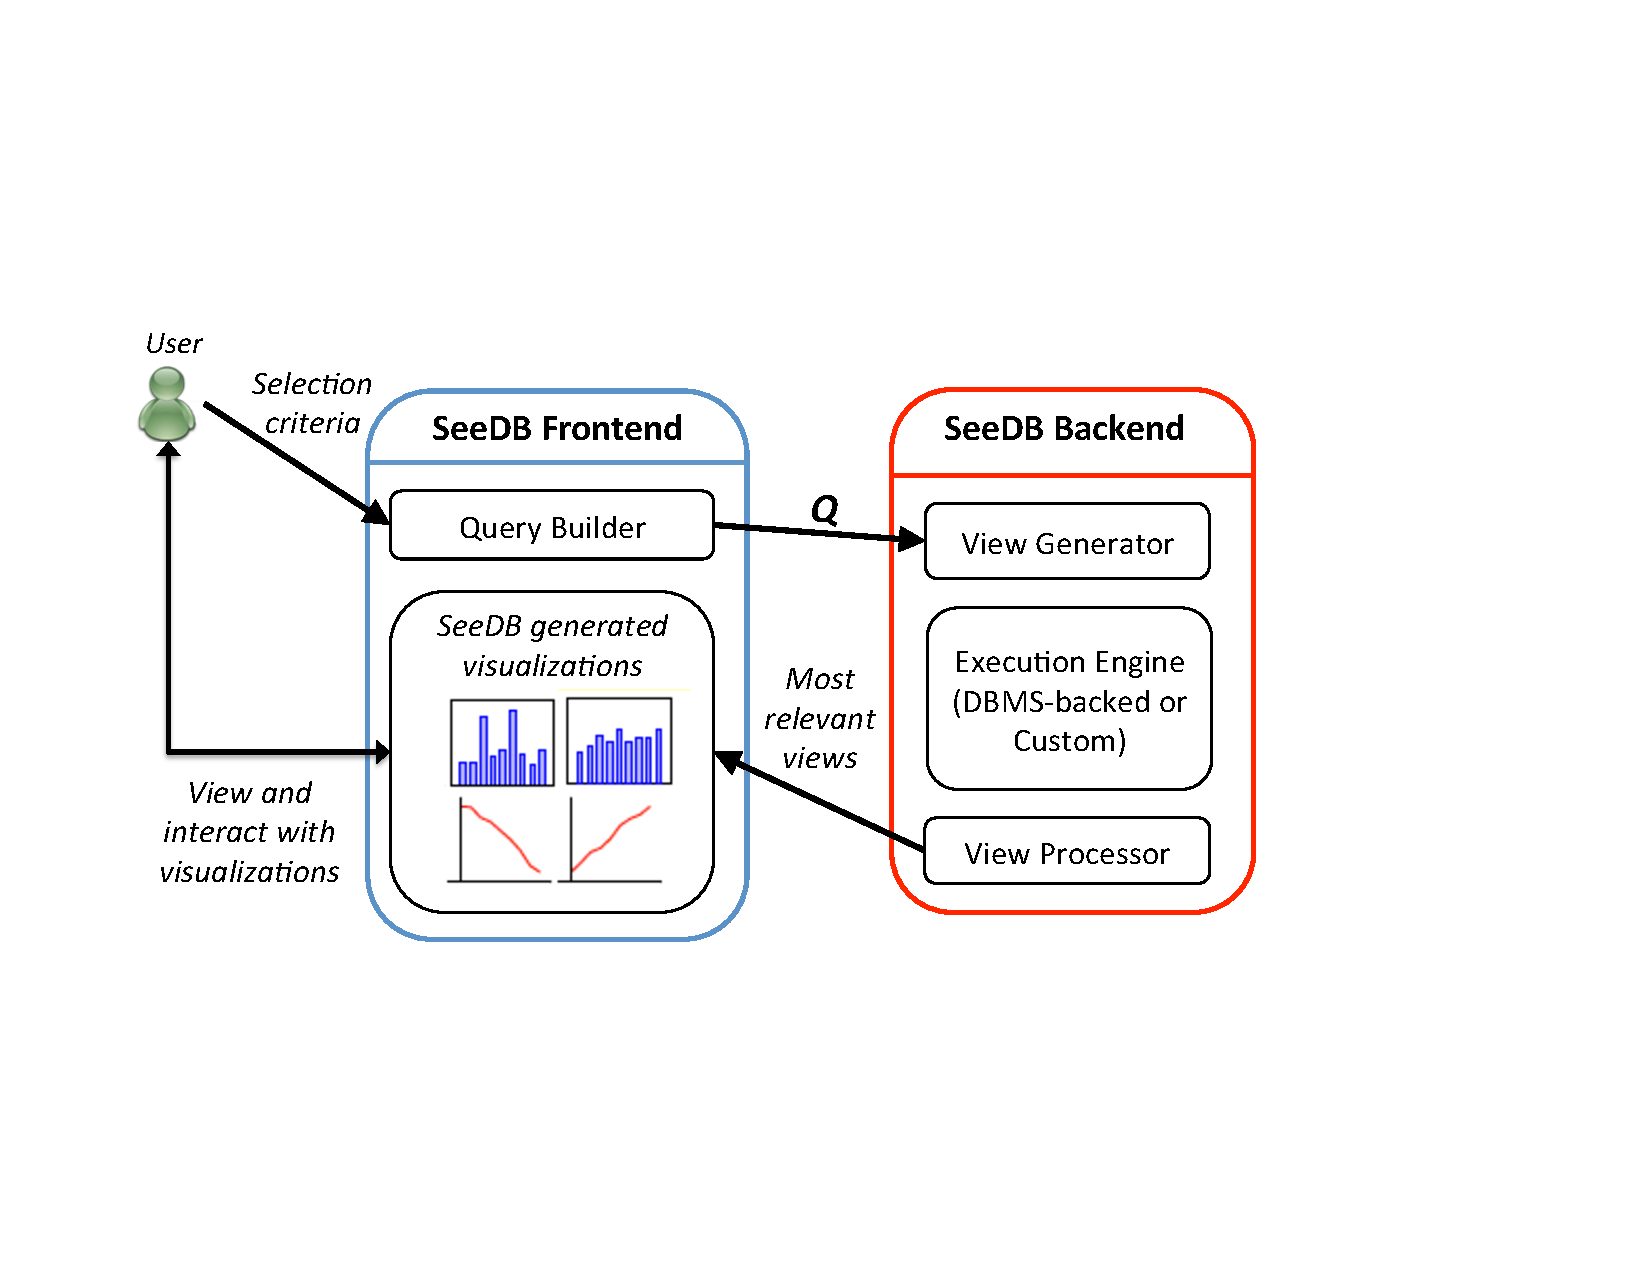
\includegraphics[trim=0 0 0 0, 
clip=true]{Images/seedb-architecture.pdf}}}}
\vspace{-12pt}
\caption{SeeDB Architecture}
\vspace{-10pt}
\label{fig:sys-arch}
\end{figure} 


\stitle{Architectural Overview.} 
\SeeDB is implemented as a middleware layer that can run on
top of any SQL-compliant database system. 
Figure \ref{fig:sys-arch} depicts the overall architecture of our
system.  The \SeeDB client is a web-based front-end that captures user
input and renders visualizations produced by the \SeeDB server.  The
\SeeDB server is composed of two main components. The first
component, the {\it view generator}, is responsible for parsing the
input query, querying system metadata and generating the list of
visualization queries that must be evaluated.  
The goal of the {\em execution engine} is to evaluate the collection of queries
 using our optimizations on top of
the underlying DBMS.
The selected aggregate views (i.e., those with high deviation) 
are sent to the \SeeDB client 
and are displayed as visualization recommendations to the user, 
who can then interact with these
visualizations.

\stitle{Basic Execution Engine.} 
To motivate the need for optimizations, we first describe 
how our execution engine would work without optimizations. 
To identify the $k$ best aggregate views,
\SeeDB needs to do the following:
For each aggregate view, it generates
a SQL query corresponding to the target
and reference view, and issues
the two queries to the underlying DBMS.
It repeats this process for each aggregate view.
As the results are received, it computes the
distance between the target and reference view
distributions, and identifies the $k$ visualizations
with highest utility. 

This basic implementation has many inefficiencies.
In a table with $a$ dimensions, $m$ measures, and $f$ aggregation functions, 
$2\times f \times a \times  m$ queries must be executed.  
As we show in Section~\ref{sec:experiments}, this can take >100s for
 large data sets.
Such latencies are unacceptable for interactive use.

\stitle{Execution Engine with Optimizations.} 
To reduce latency in 
evaluating the collection of aggregate views, 
the execution engine  
applies two kinds of optimizations:
{\em sharing}, where aggregate view queries are combined to share computation
as much as possible, and {\em pruning}, where aggregate view queries
corresponding to low utility visualizations are dropped from consideration without scanning the whole
dataset.
These optimizations are largely orthogonal to each other.
To derive benefits from both these kinds of optimizations,
we develop a {\em phased execution framework}.
Each phase operates on a subset of the dataset.
Phase $i$ of $n$ operates on the $i$th of $n$ equally-sized partitions of the dataset. 
(Empirically, we have found $n=10$ to
work well, though our results are not very sensitive to the value
of $n$.) 
For instance, if we have $100,000$ records and $10$ phases,
the $i = 4$th phase processes records $30,001$ to $40,000$.
The execution engine begins 
with the entire set of aggregate views under consideration.
\begin{denselist}
\item During phase $i$, the \SeeDB updates partial results
for the views
still under consideration using the $i$th fraction of the dataset.
The execution engine applies {\em sharing-based optimizations}
to minimize scans on this  $i$th fraction of the dataset.
\item At the end of phase $i$, the execution engine uses 
{\em pruning-based optimizations} to determine which aggregate views to discard.
The partial results of each aggregate view on the fraction from $1$ through $i$ are used to 
estimate the quality of each view, and the views with low utility are discarded. 
\end{denselist}
The retained aggregate views are then processed on the $i+1$th round,
and the process continues. 
In this manner, the set of views under consideration
decreases across these phases, with all aggregate views at the start 
of the first phase, and only the $k$ views left
at the end of the $n$th phase.
%Further, in this manner, the sharing and pruning based optimizations do
%not interfere with each other---one is applied during the phase,
%and one is applied at the end of the phase.
\papertext{The pseudocode for the phase based execution framework
can be found in the technical report~\cite{seedb-tr}.}

%We next describe the \SeeDB optimizations,
%specifically, the sharing based optimizations in Section~\ref{sec:sharing_opt} and 
%the pruning based optimizations in Section~\ref{sec:pruning_opt}.
\techreport{
\begin{algorithm}[h]
\caption{Pruning Framework}
\label{algo:custom_exec_engine}
\begin{algorithmic}[1]
\State viewsInRunning $\gets$ \{all views\}
\State currPhase $\gets$ 0
\While {currPhase.hasNext()}
\State processNextPartition()
%\State updateUtilityEstimates()
\If {currPhase.End()}
\State pruneViews(viewsInRunning)
\State currPhase.Next()
\EndIf
% \If {stoppingCondition.True()}
% \State break
% \EndIf
\EndWhile
\State return viewsInRunning.sort().getTopK()
\end{algorithmic}
\end{algorithm}
\agp{I've pasted this as is but needs to be updated.}
}
% \reviewer {
% 	D2.5 The horizontal partitioning is never detailed: how is it done? How is the
% number of fragments decided?
% }
% \mpv{something about how partitions are defined}




 
\begin{figure}[htb]
\centerline{
\hbox{\resizebox{8.5cm}{!}{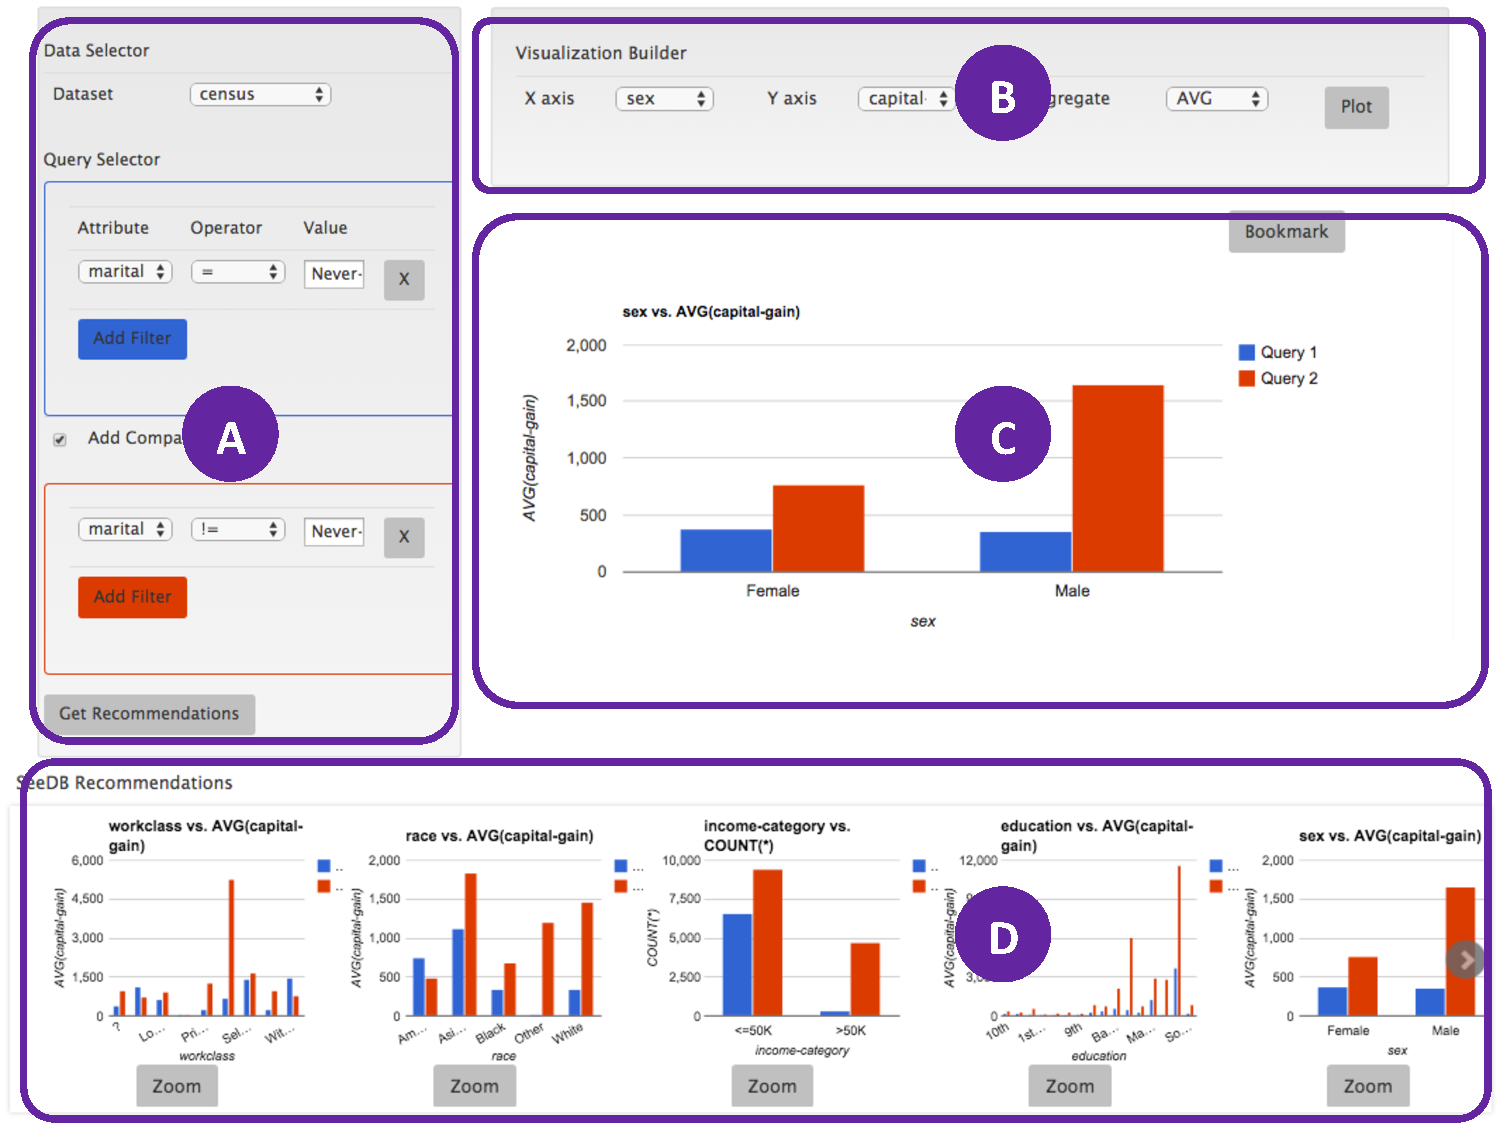
\includegraphics[trim=0mm 0mm 0mm 0mm,
clip=true]{Images/seedb_frontend.pdf}}}}
\caption{\SeeDB Frontend}
\vspace{-20pt}
\label{fig:frontend1}
\end{figure} 


% The optimizer applies multi-query
% optimization 
%  which is responsible for applying multi-query 
% optimization (Section \ref{}) to combine and rewrite DBMS queries 
% corresponding to view in running.
% Next, the execution engine issues optimized queries to the underlying DBMS
% and performs post-processing to compute results for individual views.
% Results from the execution engine are then fed to the pruner which leverages
% view pruning techniques to discard low-utility views.
% The set of views that pass muster with the pruner re-enter the optimizer for
% the next phase of execution.
% Once \SeeDB has identified the top views, the results are returned to the client 
% where \SeeDB frontend generates and displays the recommended visualizations.

% the view generator module queries the system metadata for table sizes, 
% column types, and correlations between column values. 
% It then uses this metadata and the incoming query to remove redundant aggregate views and generate ``stubs'' for the remaining aggregate views.
% The view stubs are then passed to the execution engine which is responsible 
% executing the aggregate views and performing run-time view pruning to identify
% high-utility views.
% To execute aggregate views, the execution engine optimizes the set of aggregate
% views, turns view stubs into SQL queries, and uses the underlying DBMS to efficiently execute the aggregate queries. \mpv{Fix sentence}.
% Once the \SeeDB server has executed the aggregate views and identified the top-k
% views, the data underlying top views is sent to the client where \SeeDB frontend 
% generates and displays the recommended visualizations.

% However, in this work, for ease of development and testing, we built 
% \SeeDB as a standalone end-to-end system that allows users to pose 
% arbitrary queries over data and obtain recommended visualizations.

% The standalone version of \SeeDB\ is comprised of two main components: 
% a light-weight client that is 
% used to issue queries, display recommended visualizations, and allow basic 
% interactions with visualizations; 
% and a server used to generate candidate
% aggregate views, execute
% them over data and identify the aggregate views with highest utility. 
% Figure \ref{fig:sys-arch} depicts the architecture of our system.
% Once the analyst chooses the data of interest (by issuing a query $Q$), the
% client makes a call to the backend for visualization recommendations for $Q$.
% Aggregate view stubs are essentially more elaborate triples of the form $(a, m, f)$ as discussed in Section \ref{sec:problem_statement}. 


% The generated aggregate view stubs are then sent to the execution engine
% responsible for querying the underlying data, evaluating the utility of each
% candidate view, and identifying the top views of interest. 

% Figure \ref{fig:frontend1} shows the \SeeDB client in action; including the supported mechanisms to specify an input query 
% and the visualizations generated by a sample query. 

% In the backend, the view generator module queries the system metadata for table sizes, 
% column types, and correlations between column values. 
% It then uses this metadata and the incoming query to remove redundant aggregate views and generate ``stubs'' for the remaining aggregate views. 
% Aggregate view stubs are essentially more elaborate triples of the form $(a, m, f)$ as
% discussed in Section \ref{sec:problem_statement}. 
% The generated aggregate view stubs are then sent to the execution engine
% responsible for querying the underlying data, evaluating the utility of each
% candidate view, and identifying the top views of interest. 
% Once the \SeeDB\ backend has identified the best aggregate views, the \SeeDB\
% client generates and displays recommended visualizations based on these views.
% Figure \ref{fig:frontend1} shows the \SeeDB client in action; including the supported mechanisms to specify an input query 
% and the visualizations generated by a sample query. 



% In this paper, we build the execution engine in three stages. 
% In the first stage \mpv{better word?}, we implement \SeeDB as a layer on top of the database system and apply traditional multi-query optimization 
% techniques to see how far we can push existing relational databases to support a \SeeDB-type workload.
% While we obtain resonable performance for small datasets, we find the optimizations are insufficient to support large datasets \mpv{quantify?}.
% Therefore, next, we develop a set of pruning techniques that can use running estimates of utility to rapidly prune low-utility views. 
% By reducing the number of views evaluated, these techniques reduce overall latency and also allow \SeeDB to return results without processing the entire dataset.
% We implement these pruning strategies in a simple shared scan system to test the efficacy of our techniques.
% Finally, we build a hybrid execution engine that combines our pruning strategies with the performance optimizations of the DBMS-backed execution engine,
% thus giving us the best of both worlds. 

% In this paper, we explore two distinct implementations of the \SeeDB\ execution
% engine. 
% Our first implementation draws upon traditional multi-query optimization~\cite{}
% and OLAP literature~\cite{} to implement \SeeDB\ as a wrapper
% on top of a database system. \mpv{These techniques are usually inside the DBMS, 
% we are using them outside?}
% The goal of this implementation is to study how far 

% While we obtain reasonable performance by employing well-known optimizations, we find that 
% operating through the SQL interface limits the performance we can obtain.
% Therefore, we next built a custom execution engine that completely shares query scans between
% all views and uses heuristics to rapidly prune low-utility views.
% These techniques allow us to perform only a single pass over the data
% and rapidly identify top visualizations. \mpv{Incorp into DB?}
% However, existing systems do not provide a good means to share scans between
% queries or to access intermediate results during scans.
% As a result, optimization opportunities are limited.
% To overcome the constraints of existing database systems, we implement a
% simple, custom Execution Engine for \SeeDB\ optimized to share scans
% across all views and perform pruning based on intermediate results. 
% In an ideal solution, shared scans and pruning would be implemented inside the
% database; however, for the purpose of this work, we implement the \SeeDB\
% execution engine as a standalone proof-of-concept with a brief discussion of how
% the \SeeDB\ engine could be made part of a DBMS. \mpv{need to add this discussion 
% somewhere}

% Next we briefly examine the \SeeDB client and then describe the execution engines
% in detail.

% In the DBMS-based execution engine (Section \ref{}), the view stubs are passed
% through the optimizer that identifies the best ways to combine the queries to minimize
% execution time.
% Once the views have been optimized, the views are rewritten as SQL queries and
% executed against the underlying database. 
% The results of these queries are
% processed to update the view stubs and compute view utility. 
% Once all the queries have been processed, the top-k views are returned to the
% frontend.
% 
% In the main-memory execution engine, \SeeDB\ makes a single pass through the
% data (either read from disk or already present in memory) and keeps running
% estimates of utility for each of the views stubs obtained from the View
% Generator. 
% As the engine processes more of the data, the utility estimates become more
% accurate and \SeeDB\ uses various pruning heuristics to prune out views on the fly.
% By the time the full data has been processed, \SeeDB\ has identified the top-k
% views with the largest utility that are then returned to the frontend.



 %!TEX root=document.tex


\section{VizRecDB Frontend}
\label{sec:VizRecDB_frontend}

The \VizRecDB\ frontend, designed as a thin client, performs two main functions: it
allows the analyst to issue a query to \VizRecDB, 
and it visualizes the results (views) produced by the \VizRecDB\
backend.
To provide the analyst maximum flexibility in issuing queries, \VizRecDB\
provides the analyst with three
mechanisms for specifying an input query: 
(a) directly filling in SQL into a text box, 
(b) using a query builder tool that allows analysts
unfamiliar with SQL to formulate queries through a form-based interface, and (c)
using pre-defined query templates which encode commonly performed operations,
e.g., selecting outliers in a particular column. 
%We find that pre-defined query
%templates are particularly useful since analysts are often interested in
%anomalous data points.

Once the analyst issues a query via the \VizRecDB\ frontend, the backend
evaluates various views and delivers the most interesting ones (based on
utility) to the frontend.
For each view delivered by the backend, the frontend creates a visualization
based on parameters such as the data
type (e.g. ordinal, numeric), number of distinct values, and semantics (e.g.
geography vs. time series).
The resulting set of  visualizations is displayed to the analyst who can then
easily examine these $k$ (user-specified) ``most interesting'' views at a glance, 
explore specific views in detail via drill-downs, 
%by hovering and clicking on various portions of the view, 
and study metadata for each view (e.g. size of result, sample data, value with
maximum change and other statistics). 
%The analyst can also slice-and-dice views further by performing drill-downs on
%specific attributes in the view. 
Figure~\ref{fig:frontend1} shows a screenshot of the \VizRecDB\ frontend (showing
the query builder and resulting visualizations) in action.
 
\begin{figure}[htb]
\vspace{-10pt}
\centerline{
\hbox{\resizebox{5cm}{!}{\includegraphics[trim=15mm 0mm 120mm 0mm,
clip=true]{Images/sql_builder.pdf}}}
\hbox{\resizebox{!}{6cm}{\includegraphics[trim=50mm 30mm 150mm 52mm,
clip=true]{Images/viz_panel.pdf}}}}
\caption{VizRecDB Frontend: Query Builder (left) and Example Visualizations
(right)}
\label{fig:frontend1}
\vspace{-10pt}
\end{figure} 

In this work, we focus on the \VizRecDB\ backend and develop techniques to
speed up identification of interesting views. As a result, we leave the
development of a more advanced and flexible \VizRecDB\ frontend for future work. 
In the next section, we describe the \VizRecDB\ execution engine and discuss
two implementations in detail.

 \section{\SeeDB Optimizer}
\label{sec:optimizer}

Each visualization evaluated by \SeeDB translates into two 
aggregation queries on the DBMS, one for the target view and one for the comparison view.
The queries corresponding to each visualization are
 similar; they scan the same underlying data,  
differing only in the  attributes used for grouping and aggregation.
As a result, there are opportunities to reduce the number of queries and passes over the data 
by merging and batching queries.
%During each phase, the \SeeDB optimizer consumes stubs
%corresponding to views still in running and produces an optimal
%execution plan that maximizes sharing opportunities.

% Each phase of execution in \SeeDB begins with the optimizer. 
% The \SeeDB optimizer takes as input view stubs $(a, m, f)$, 
% corresponding to the set of visualizations still in running during 
% a particular phase.
% The goal of the optimizer is to generate a plan that executes view
% queries as efficiently as possible.

\stitle{Baseline Plan:} When no optimization is applied, \SeeDB adopts
the following simple execution plan.
Each view $(a, m, f)$ is evaluated sequentially by running queries against the database.
For each view, individual view queries corresponding to the
target and comparison view are run independently on the DBMS.
Results of these queries are then used to compute utility for each
view.

This baseline plan has several inefficiencies.
In a table with $a$ dimensions, $m$ measures, and $f$ aggregation functions, 
$2\times f \times a \times  m$ queries must be executed independently.  
As we show in Section~\ref{sec:experiments}, executing the baseline plan can take hundreds of seconds  for
moderate sized data sets.
Consequently, the goal of the optimizer is choose a set of combined queries that
minimize the total work done by the database and produces answers across the entire
set of view.
Sharing computation in \SeeDB is a special case of the general problem
of multi-query optimization~\cite{DBLP:journals/tods/Sellis88}; we discuss the 
relationship in more detail in Section~\ref{sec:related_work}.

\reviewer {
	D2.4 Regarding the number of queries to be executed: where are the f
functions to be found? I think there is a (minor) inconsistency: if there are
a*f*m*2 queries to be executed, why in Section 4.2 do you have (a1 , m1 ,
f1 ), (a1 , m2, f2) ...(a1, mk, fk)?
}

\subsection{Optimization Strategies}
\mpv{rule-based optimization?}

%The \SeeDB optimizer maximizes re-use of computation between
%visualizations by intelligently merging the set of view queries and batching them during execution.
 \SeeDB adopts the four merging and sharing strategies.
% The \SeeDB optimizer adopts the following optimization strategies to minimize the total
% number of queries over the data and consequently the total scans of the data.

\stitle{Combine Multiple Aggregates}: Aggregate view queries 
with the same GROUP BY attribute can be 
rewritten as a single, combined query. So instead of executing
queries for views $(a_1$, $m_1$, $f_1)$, $(a_1$, $m_2$, $f_2)$ \ldots $(a_1$, $m_k$, $f_k)$
independently, \SeeDB combines them into a single view represented by
$(a_1, \{m_1, m_2\ldots m_k\}$, $\{f_1, f_2\ldots f_k\})$.  
We have found that there is minimal to no impact on latency 
to grouping as many aggregates as possible in both row and column stores. 

\stitle{Combine target and comparison view query}:
Since the target view and comparison views differ only in the subset of data
 the query is executed on, \SeeDB rewrites these two view queries as
one. For instance, the target and comparison view queries $Q1$ and $Q2$
shown below, can be combined into a single query $Q3$.
\vspace{-5pt}
\begin{align*} 
Q1 = &{\tt SELECT \ } a, f(m) \ \ {\tt FROM} \  D\  {\tt WHERE \ \ x\ <\ 10\
GROUP \ \ BY} \ a \\
Q2 = &{\tt SELECT \ } a, f(m) \ \ {\tt FROM} \  D\  {\tt GROUP \ \ BY} \ a \\
Q3 = &{\tt SELECT \ } a, f(m), {\tt CASE\ IF\ x\ <\ 10\ THEN\ 1\ ELSE\ 0\
END}\\ 
&as\ g1,\ 1\ as\ g2 \ \ {\tt FROM} \ D\ {\tt GROUP \ \ BY} \ a,\ g1,\ g2
\end{align*}

\stitle {Parallel Query Execution}:
  \SeeDB executes multiple view queries in parallel since  co-executing queries can often
 share buffer pool pages, reducing disk accesses times. 
  However, the precise number of parallel queries needs to be tuned to take into account 
  buffer pool contention, locking and cache line contention \cite{Postgres_wiki}.  We experimentally
evaluate the optimal degree of parallelism in Section~\ref{sec:experiments.}

\stitle {Combine Multiple GROUP BYs}:
% Efficient cube materialization is a problem well studied in the OLAP literature.
% Since the views considered by \SeeDB\ can be thought of as projections of the OLAP
% cube, we can adapt efficient materialization techniques to our problem.
After applying our multiple aggregate optimization, \SeeDB is left with a number of 
queries with a GROUP BY on a single aggregate.
These can be also grouped together into a single query, but each additional 
group by attribute will increase the number of groups, and (possibly) lead to slower
overall performance as the number of groups becomes large.  
Therefore, \SeeDB\ has to determine the optimal way of executing these multi-attribute
GROUP BY queries.

Our specific problem is as follows: given a space budget $\mathcal{S}$,
and estimates of sizes of views (i.e., number of rows in the result), we need to find the optimal
way to combine multiple single-attribute GROUP BY queries into multi-attribute GROUP BY queries.
If we know the number of distinct values for each attribute, we can estimate the
size of a view containing dimension attributes $a_i$ and $a_j$ as $|a_i|\times |a_j|$.
Formally, our problem becomes:
\vspace{-5pt}
\begin{problem}[Optimal Grouping]
Given a set of dimension attributes $A$ = \{$a_1$\ldots$a_n$\}, divide the
dimension attributes in $A$ into groups $A_1, \ldots, A_l$ (where $A_i$ is some
subset of $A$ and $\bigcup A_i$=$A$) such that if a query $Q$ groups the table by $A_i$, 
the total space budget for $Q$ does not exceed $\mathcal{S}$.
\vspace{-5pt}
\end{problem}

Notice that the above problem is isomorphic to the NP-Hard {\em bin-packing} problem~\cite{garey}.
If we let each dimension attribute
$a_i$ correspond to an item in the bin-packing problem with weight $\log (|a_i|)$,
and set the bin size to be $\log \mathcal{S}$,
then packing items into bins is identical to finding groups $A_1, \ldots, A_l$,
such that the estimated size of any query result is below $\mathcal{S}$.
We use the standard first-fit algorithm~\cite{first-fit} to find the optimal
grouping of dimension attributes.

\stitle{Other Optimizations}: 
To further speedup processing, \SeeDB can also pre-compute results for 
static views (e.g. comparison views on full tables) or operate on
pre-computed data samples.  Such optimizations are orthogonal to the
problem of efficiently evaluating a large number of views, which we will have to
do even in the presence of pre-computation or sampling, so we don't focus on them here.

\mpv{should we put in information of our cost function?}


 %!TEX root=document.tex

\section{View Pruning Framework}
\label{sec:pruning_framework}
% The previous section described techniques to
% batch and share computations across queries---however,
% if the number of queries is large, this can still 
% lead to high execution times.
Although it is possible to construct hundreds of potential (aggregate)
visualizations for a typical dataset, only a fraction of these visualizations have high utility and are relevant to the user.
Most visualizations are low-utility and computational resources
are wasted in computing these visualizations.
% Moreover, only a fraction of the visualizations evaluated by
% \SeeDB are of high quality; most models have low utility and
% computational resources are wasted in computing these visualizations.
In this section, we describe \SeeDB's view pruning framework used to 
eliminate many views without completely evaluating them.

\stitle{Basic Pruning Framework.}
\label{subsec:basic_framework}
Recall that the pruning algorithm executes in phases, with each phase partially evaluating optimized query batches
on a subset of the data.
Specifically, after each phase, \SeeDB estimates the utility of each view on data from the current and previous batches, and eliminates
low-utility views that are very unlikely to be in the top-$k$.  It also can accept certain views as definitely being in the top-$k$.
If more than $k$ views remain, it iterates over the next batch of data;  otherwise the top-$k$ views are returned to the front end.
This process is shown in Algorithm~\ref{algo:custom_exec_engine}.


\begin{algorithm}[h]
\caption{Pruning Framework}
\label{algo:custom_exec_engine}
\begin{algorithmic}[1]
\State viewsInRunning $\gets$ \{all views\}
\State currPhase $\gets$ 0
\While {currPhase.hasNext()}
\State processNextPartition()
%\State updateUtilityEstimates()
\If {currPhase.End()}
\State pruneViews(viewsInRunning)
\State currPhase.Next()
\EndIf
% \If {stoppingCondition.True()}
% \State break
% \EndIf
\EndWhile
\State return viewsInRunning.sort().getTopK()
\end{algorithmic}
\end{algorithm}


We implemented two different pruning schemes in \SeeDB.
The first scheme uses  confidence-interval
techniques to bound utilities of views, while the second uses
multi-armed bandit allocation strategies to find top utility views.

\stitle{Confidence Interval-Based Pruning.}
\label{sec:confidence_interval}
This pruning scheme uses worst-case statistical confidence intervals to bound utility estimates obtained as \SeeDB
processes larger fractions of the underlying dataset.
Our pruning technique is similar to top-k based pruning 
algorithms developed 
in other contexts as described in ~\cite{DBLP:conf/pods/FaginLN01, 
DBLP:conf/vldb/IlyasAE04, DBLP:conf/ICDE/ReDS07}.

Pruning works as follows: at every point during execution, \SeeDB
maintains a running estimate of the mean utility $u_i$ for every view 
$V_i$ and a confidence interval around that mean, $u_i \pm c_i$.	

At the end of a phase, we use the estimates $u_i \pm c_i$ to prune low-utility views according to the following rule:
{\em If the upper bound of the utility of view $V_i$ is lesser
than the lower bound of the utility of $k$ or more views, then $V_i$ is discarded.}
To illustrate, suppose a dataset has four views $V_1$ to $V_4$ and we wish to find the top-$2$ views.
Further suppose that at the end of phase $p$,
$V_1$-$V_4$ have utility confidence intervals as shown in Figure \ref{fig:conf_interval}.
Views $V_1$ and $V_2$ have the highest estimates for utility so far.
Consider view $V_3$; we see that $V_3$'s confidence interval overlaps with the
confidence intervals of the current top views, making it possible
that $V_3$ will be in the final top views. On the other hand, the confidence
interval for $V_4$ lies entirely below the lowerbounds of $V_1$ and $V_2$.
Since we can claim with high probability
that the utility of $V_4$ lies within its confidence interval, it follows that
with high probability, $V_4$'s utility will be lower than that of both $V_1$ and
$V_2$, and it will not appear in the top-$2$ views.
We state the algorithm formally in
Algorithm~\ref{algo:ci_based_pruning}.

\begin{figure}[h]
\vspace{-10pt}
\centerline{
\hbox{\resizebox{8cm}{!}{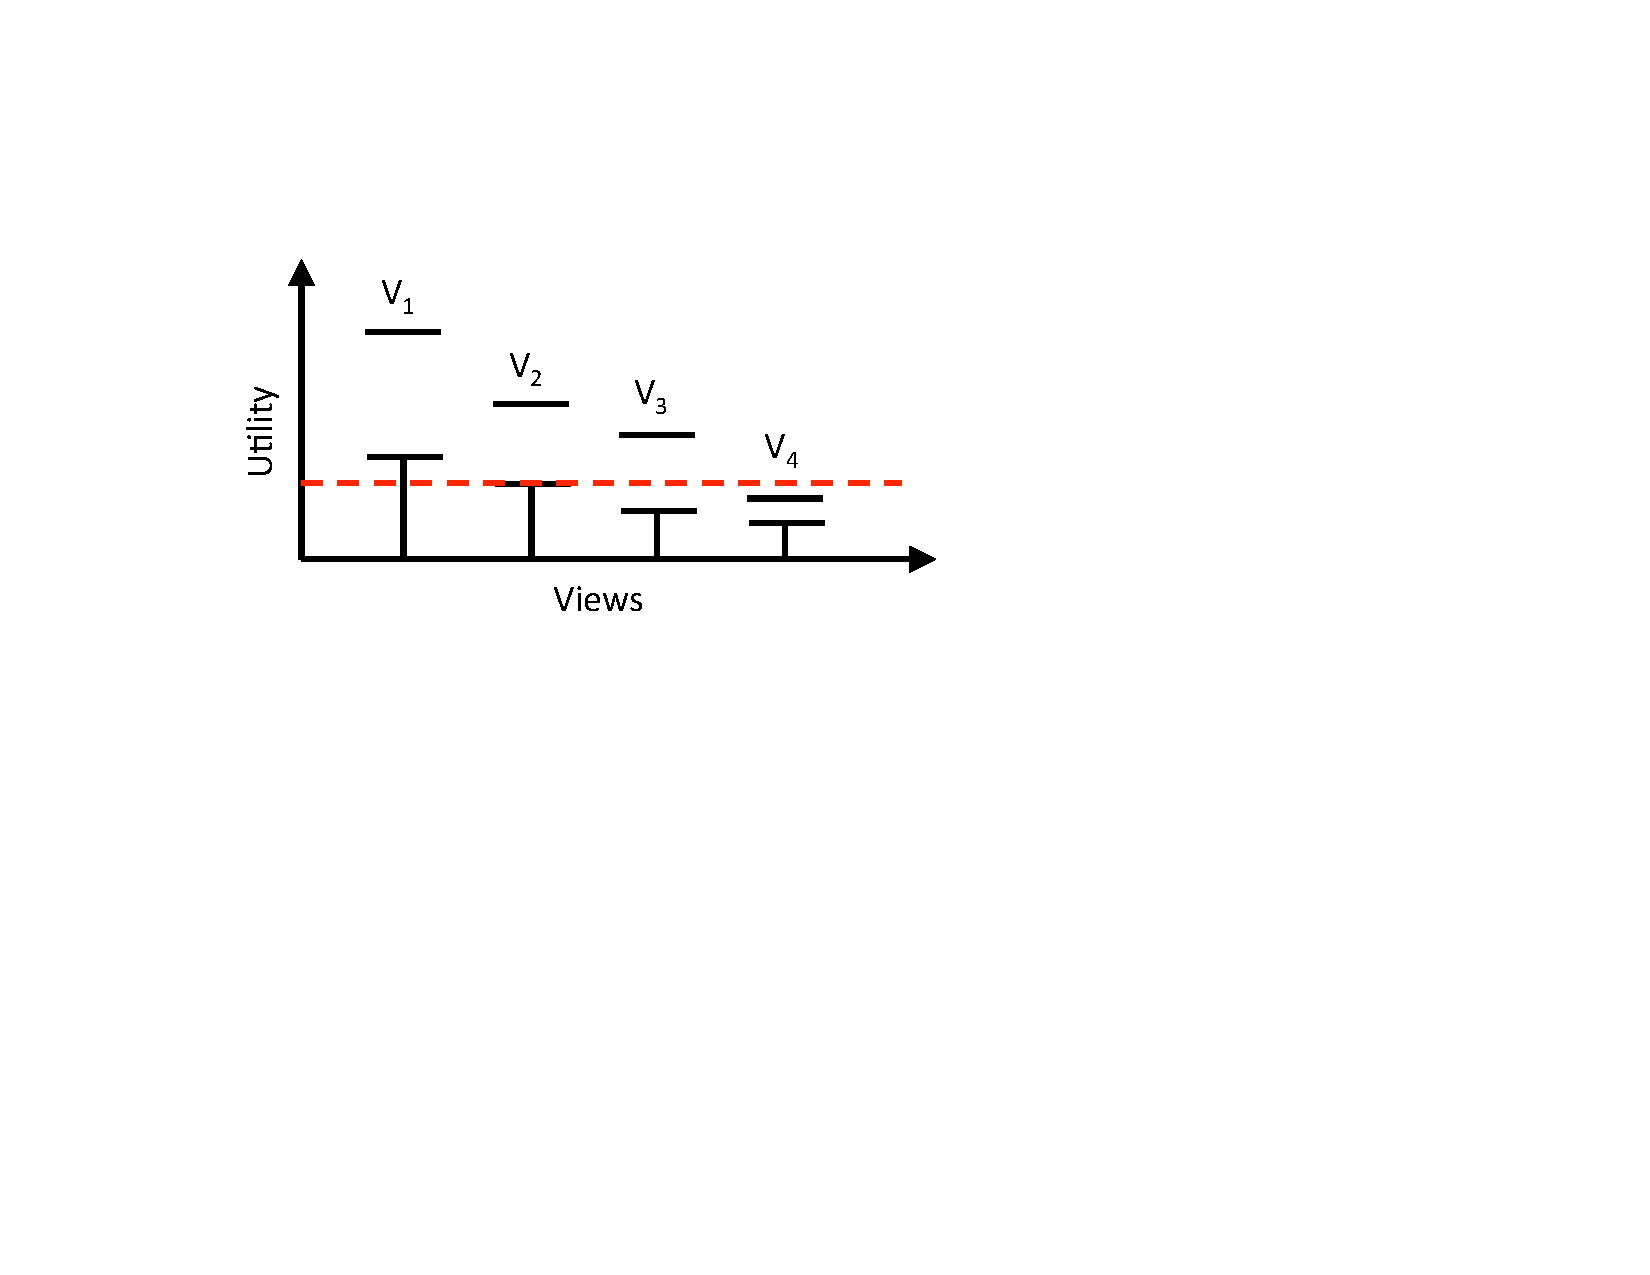
\includegraphics[trim=10mm 100mm 55mm 35mm, 
clip=true]{Images/confidence_pruning.pdf}}}}
\vspace{-20pt}
\caption{Confidence Interval based Pruning}
\label{fig:conf_interval}
\vspace{-15pt}
\end{figure}

\reviewer {
	V5 is extraneous
}


% \papertext{Pseudocode for our pruning scheme can be found in our technical report~\cite{seedb-tr}.}

\begin{algorithm}
\caption{Confidence Interval Based Pruning}
\label{algo:ci_based_pruning}
\begin{algorithmic}[1]
\State viewsInRunning.sortByUpperbound()
\State topViews $\gets$ viewsInRunning.getTopK()
\State lowestLowerbound $\gets$ min(lowerbound(topViews))
\For {view $\not \in$ topViews}
\If {view.upperbound < lowestLowerbound}
\State viewsInRunning.remove(view)
\EndIf
\EndFor
\end{algorithmic}
\end{algorithm}

To obtain conservative bounds, we use {\it worst case} confidence intervals as derived from
the Hoeffding-Serfling inequality~\cite{serfling1974probability}.
The inequality states that if we are given $N$ values $y_1, \ldots, y_N$ in 
$[0, 1]$ with average $\mu$, and we have have drawn $m$ values without replacement, $Y_1, \ldots, Y_m$, 
then we can calculate a running confidence interval around the current mean 
of the $m$ values such that the actual mean of the $N$
is always within this confidence interval with a probability of $1 - \delta$:
\begin{theorem}
\label{thm:hs}

Fix any $\delta > 0$. For $1 \le m \le N-1$, define
{\small $$
\varepsilon_m = \sqrt{\frac{(1-\frac{m-1}N)(2\log \log (m) + \log(\pi^2/3\delta))}{2m}}.
$$
$$
\textrm{Then:} \ \   \Pr\left[ \exists m, 1 \le m \le N : 
  \left|\frac{\sum_{i=1}^m Y_i}{m} - \mu\right| > \varepsilon_m \right] 
\le \delta.
$$
}

\end{theorem}
In our setting, each $Y_i$ corresponds to an estimate of utility computed based on the
records seen so far. 


\stitle{Multi-Armed Bandit Pruning.}
\label{sec:multi_armed_bandit}
%The \SeeDB pruning problem seeks to start with a large set of potential
%visualizations and to rapidly narrow them at run-time to the set of 
%visualizations with the highest utility.
Our second pruning scheme uses an adapative of a Multi-Armed Bandit (MAB)~\cite{bandits, AuerCF02, LaiR85} to identify top views.
In MAB, an online algorithm chooses from a set of alternatives (arms)
 over a sequence of trials to maximize reward.  In our setting,the  alternatives correspond to various visualizations and the reward corresponds
 to utility. 
We note that this is the first time that bandit strategies have been
applied to the problem of identifying interesting visualizations.

\techreport{The setting of MAB is as follows: a gambler is faced with several slot
machines (``one-armed bandit''s), each of which has an underlying 
(unknown) reward distribution. 
Every play results in a reward from the corresponding machine's
reward distribution.
The goal is to devise a {\it strategy} of which machine to play
at each turn in order to maximize the reward~\cite{bandits}.}
A recently-studied variation of MAB focuses on finding the arms with the highest
mean rewards~\cite{BubeckWV13, audibert2010best}.
Under certain \srm{which?} assumptions, this variation is identical to the problem addressed by \SeeDB: our goal is find the views (arms) with the 
highest utility. \mpv {is it arms or bandits?}.
Specifically, we adapt the Successive Accepts and Rejects algorithm from \cite{BubeckWV13} 
to find arms with the highest mean reward. 
Algorithm~\ref{algo:mab_based_pruning} shows the pseudocode for our pruning technique.
% As before, the processing of the input table is divided into phases.
% In every phase, \SeeDB\ reads in new records and updates the distributions and utilities
% for every view in the running.
At the end of every phase, all {\it active} views are ranked in order of their utility means. 
We then compute two special differences between the utility means: $\Delta_1$
is the difference between the highest mean and the $k+1$st highest mean, and
$\Delta_n$ is the difference between the lowest mean and the $k$th highest mean.
If $\Delta_1$ is greater than $\Delta_n$, the view with the highest mean is
``accepted'' as being part of the the top-$k$ (and it no longer participates
in pruning computations).
On the other hand, if $\Delta_n$ is higher, the view with the lowest mean is discarded
from the set of views in the running.
\cite{BubeckWV13} proves that under certain assumptions about reward distributions,
the above technique identifies the top-$k$ arms with high probability.
\mpv{put guarantee?}

\reviewer{
	For the MultiArmed
Bandit pruning, it would be good to discuss whether
the assumptions of reward distributions would necessarily in this context.
}
\mpv{
	The MAB setting assumes that each trial samples from the same 
	underlying reward distribution, which is the reward distribution
	computed after processing all records. In our setting, however, 
	the underlying reward distribution changes gradually as we
	process more records and tends towards the {\em true} reward
	distribution.
	We assume that these changes to the distributions are small.
}
\srm{Are we sure the above paragraph is correct?  Since we have random samples, I don't see 
why the reward distribution is changing.  Shouldn't it be the same?}

\begin{algorithm}
\caption{MAB Based Pruning}
\label{algo:mab_based_pruning}
\begin{algorithmic}[1]
\State viewsInRunning.sortByUtilityMean()
\State \{$\bar{u}_{i}$\} $\gets$ sorted utility means
\State $\Delta_1$ $\gets$ $\bar{u}_{1}$ - $\bar{u}_{k+1}$
\State $\Delta_n$ $\gets$ $\bar{u}_{k}$ - $\bar{u}_{n}$
\If {$\Delta_1$ < $\Delta_n$}
\State viewsInRunning.acceptTop()
\Else
\State viewsInRunning.discardBottom()
\EndIf
\end{algorithmic}
\end{algorithm}

\mpv{Guarantees from this technique?}

\stitle{Early Stopping.}
Both of these techniques can frequently estimate the top-$k$ views before the entire dataset has been scanned.
At this point, we can either continue to scan the entire data set to generate a completely accurate
picture of these $k$ views, or we can emit an approximation of these $k$ views immediately.  We show 
in our experiments that this {\it early stopping} can significantly improve the runtime of our pruning algorithms.

\subsection{Extension to Other Utility Metrics}

\mpv{should we say something here? Something like none of our
algorithms depend on the specific properties of EMD.
In fact, these techniques apply to any consistent estimator.
}

\mpv{
	Aditya: can you take a stab at this part?
}

%Note that the two pruning schemes described above have guarantees
%in other settings that do not directly carry over to our setting.
In our evaluation, we show that the above  pruning schemes
work  well in practice. 
We can also prove, however,  that as we sample more and more, the estimated utility
$\hat{U}$ (\srm{for both pruning techniques?}) will coverge towards to $U$ for all aggregate views.
We can state our claim formally in the following lemma. 
\papertext{The proof based on 
Hoeffding's inequality can be found in the extended
technical report ~\cite{seedb-tr}.}
\techreport{The proof of this lemma is presented in Section \ref{sec:convergence}.}
% At a high level, the proof
% involves repeated applications of Hoeffding's inequality to
% upper and lower-bound $\hat{U}$ within $U$ along with terms 
% that tend to $0$ as the number of samples increases.

\begin{lemma}
Let the target and comparison visualizations
both have $m$ groups.
Let $\hat{U}$ denote our estimate of $U$ based on a uniformly random sample 
across all $m$ groups. 
Then, as the number of samples tends to $\infty$, $\hat{U} \rightarrow U$
with probability $1-\delta$, for any desired $\delta$.
\end{lemma}
 %%!TEX root=document.tex
\section{{\large \SeeDB\ } Execution Engine}
The goals of the \SeeDB execution engine are to efficiently
compute the utility of a large number of aggregate views
and to then find and display the $k$ visualizations with the highest utility.

\subsection{Basic Implementation} \label{sec:dbms-exec-engine}

We now describe the basic implementation of \SeeDB
over a traditional relational database system.
Recall that the input to the \SeeDB engine is a set of 
aggregate view stubs, i.e., triples of the form
$(a, m, f)$, where $a$ is the dimension attribute, $m$ is the measure,
and $f$ is the aggregation function.
For each aggregate view stub, we craft
a SQL query corresponding to the target
and comparison view, and issue
the two queries, one at a time, to the database.
We then repeat this for each aggregate view stub.
As the results are obtained, we can compute the
distance between the target and comparison view
distributions, and keep track of the $k$ visualizations
with highest utility. These are then displayed
to the analyst.


Naturally, this basic implementation has many inefficiencies.
In a table with $a$ dimensions, $m$ measures, and $f$ aggregation functions, 
$2\times f \times a \times  m$ queries must be executed independently.  
As we show in Section~\ref{sec:experiments}, this can take minutes in
large data sets (with hundreds of attributes and millions of rows), which is too long for interactive use. \mpv{are we at interactive time scales?}
We propose two different suites of optimizations to deal with these
inefficiencies.
The first suite of optimizations, discussed in Section~\ref{sec:sharing-opt}, concerns {\em sharing}, \mpv{grouping sets are the other end of sharing}
i.e., sharing as much work as possible while leveraging the 
backend database system.
The second suite of optimizations, discussed in Section~\ref{sec:in_memory_execution_engine}, concerns {\em pruning},
i.e., avoiding the complete computation of some aggregate views
by pruning them away. The second suite of optimizations
are approximate, in that they, since they use utility estimates, there is a small likelihood that the returned visualizations may not have the highest utility.
%  in rare occasions may lead
% to inaccurate results (in that the visualizations
% displayed need not be the ones with the best utilities).

% Our first instantiation of the \SeeDB\ engine uses SQL queries in a
% traditional database system to evaluate the utility of each view.
% %We explore this design because it enables \SeeDB\ to be easily integrated 
% %with visualization systems that use DBMSs for data storage (e.g. Tableau, 
% %Spotfire etc).
% The advantage of this design is that it benefits
% from all the features of a standard relational engine and can be easily integrated into systems
% that use DBMSs for data storage.
% However, the efficiency of this approach is somewhat limit because
% the only way to interact with data is via SQL queries.
% %On the downside, this design limits \SeeDB\ to using the API
% %exposed by the DBMS; essentially, 
% %\SeeDB\ can only open/close connections to the
% %database and execute one or more SQL queries. 
% %Since we have no control over how queries are executed or access to intermediate
% %results, 

% Given a set of view stubs provided to the execution engine, conceptually,
% the basic approach proceeds as follows:
% (1) for each view, we generate SQL queries for the target and
% comparison view---recall that these are aggregate queries, where
% the target view is the aggregate query corresponding 
% to the visualization being considered, and the comparison
% view is the aggregate query that is being compared against,
% for the purpose of utility computation;
% see Section \ref{sec:problem_statement}, 
% (2) we execute each view query independently on the DBMS, 
% (3) the results of each query (i.e. the aggregated values) are processed and
% normalized to compute the target and comparison distributions, 
% (4) we compute utility for each view 
% and select the top-$k$ views with the largest utility,
% which are then sent to the frontend.
% This strawman approach is clearly inefficient since it examines every possible view and 
% executes each view query independently.

\subsection{Sharing-Based Optimizations}\label{sec:sharing-opt}
In this section, we focus on minimizing total execution time
by reducing the
total number of queries issued to the database,
and by reducing the total number of scans of the underlying table.
Specifically, we apply the following optimizations:
\agp{I didn't make a smoothing pass on the rest of this..}

\stitle{Combine Multiple Aggregates}: All aggregate view queries 
with the same group-by attribute can be 
rewritten as a single, combined query. So instead of executing
queries for views $(a_1$, $m_1$, $f_1)$, $(a_1$, $m_2$, $f_2)$ \ldots $(a_1$, $m_k$, $f_k)$
independently, we combine them into a single view represented by
$(a_1, \{m_1, m_2\ldots m_k\}$, $\{f_1, f_2\ldots f_k\})$.  We have found that there is no penalty
to grouping as many aggregates as possible in both row and column stores. 

\stitle{Combine target and comparison view query}:
Since the target view and comparison views only differ in the subset of data
that the query is executed on, we rewrite these two view queries as
one. For instance, the target and comparison view queries $Q1$ and $Q2$
shown below, can be combined into a single query $Q3$.
\vspace{-5pt}
\begin{align*} 
Q1 = &{\tt SELECT \ } a, f(m) \ \ {\tt FROM} \  D\  {\tt WHERE \ \ x\ <\ 10\
GROUP \ \ BY} \ a \\
Q2 = &{\tt SELECT \ } a, f(m) \ \ {\tt FROM} \  D\  {\tt GROUP \ \ BY} \ a \\
Q3 = &{\tt SELECT \ } a, f(m), {\tt CASE\ IF\ x\ <\ 10\ THEN\ 1\ ELSE\ 0\
END}\\ 
&as\ g1,\ 1\ as\ g2 \ \ {\tt FROM} \ D\ {\tt GROUP \ \ BY} \ a,\ g1,\ g2
\end{align*}

\stitle {Parallel Query Execution}:
  We execute multiple view queries in parallel since we expect co-executing queries 
  to share buffer pool pages and reduce disk accesses times. 
  However, the precise number of parallel queries needs to be tuned to take into account 
  buffer pool contention, locking and cache line contention \cite{Postgres_wiki}. 
  %As a result, we must identify the optimal number of parallel queries for our workload.

% We can do much better if we can use a single scan to evaluate multiple views simultaneously.

% In fact, our ideal operator $\mathcal{O}$ would perform a single scan of the
% data and compute all query results in one pass to return the top-$k$ views.
% Current database systems do not support this functionality.
% A handful of systems have recently introduced the SQL GROUPING
% SETS\footnote{GROUPING SETS allow the simultaneous grouping of query results by
% multiple sets of attributes.} functionality that could be used to support this
% operation. However, the grouping sets operator will not scale to tables with 
% a large number of attributes due to the large size of intermediate results.
% size of the eventual result maintained in memory will be $2 \times a \times f
% \times m$ attributes, multiplied by the size of an aggregate distribution.
% Furthermore, as we show in Section \ref{sec:in_memory_execution_engine},
% evaluating all views for the entire dataset is unnecessary and inefficient. 
% We can achieve much better performance by aggressively pruning low-utility
% views on the fly.

% Without this ideal operator $\mathcal{O}$,
% our optimizations minimize table scans in two ways: (1) minimize the total number of
% queries by intelligently combining queries, and (2) reduce the total
% execution time by running queries in parallel. 
% Our DBMS-backed execution engine for \SeeDB\ is agnostic towards the
% particular DBMS used to execute queries.
% However, because of significant differences in the way that row stores and
% column stores organize data, some of the optimizations described below
% will be more powerful in row stores and may actually hurt performance in column
% stores. In our experimental evaluation (Section \ref{sec:experiments}), we study
% the relative advantages of each of our optimizations for row and column stores.
% The optimizations supported by \SeeDB\ are described below.

% \subsubsection {Combine Multiple Aggregates} 
% A large number of view queries have the same group-by attribute but different
% aggregation attributes. 
% Therefore, \SeeDB\ combines all view queries with the same
% group-by attribute into a single, combined view query. For instance, instead of executing
% queries for views $(a_1$, $m_1$, $f_1)$, $(a_1$, $m_2$, $f_2)$ \ldots $(a_1$, $m_k$, $f_k)$
% independently, we can combine the $n$ views into a single view represented by
% $(a_1, \{m_1, m_2\ldots m_k\}$, $\{f_1, f_2\ldots f_k\})$. We demonstrate later
% on (Section \ref{sec:expts_dbms_execution_engine})  that this optimization
% offers a speed-up roughly proportional to the number of measure attributes.

\stitle {Combine Multiple Group-bys}:
% Efficient cube materialization is a problem well studied in the OLAP literature.
% Since the views considered by \SeeDB\ can be thought of as projections of the OLAP
% cube, we can adapt efficient materialization techniques to our problem.
After applying our multiple aggregate optimization, we are left with a number of 
queries with a group-by on a single aggregate.
We can of course group these together into a single query, but but each additional 
group by attribute will increase the number of groups, and (possibly) lead to slower
overall performance when the number of groups becomes large.  
Therefore, \SeeDB\ has to determine the optimal way of executing these multi-attribute
{\it group-by} queries.
%Savvy readers will recognize this problem as being a special case of materializing
%an OLAP cube~\cite{olap_cube}.
%Views evaluated by \SeeDB\ are projections of the OLAP cube and we can adapt techniqes
%from the cube literature~\cite{} to find the optimial execution strategy for these queries.
% There are few differences in the \SeeDB\ setting and traditional OLAP cubes: (1) OLAP
% cube materialization is performed inside the database giving more flexibility in the
% techniques used; in \SeeDB\ every evaluation corresponds to a separate query; (2) 
%Specifically, we work with a similar problem formulation: 
Our specific problem is as follows: given a space budget $\mathcal{S}$,
and estimates of sizes of views (i.e. number of rows in the result), we need to the optimal
way to combine multiple single-attribute group-by queries into multi-attribute group-by queries.
If we know the number of distinct values for each attribute, we can estimate the
size of a view containing dimension attributes $a_i$ and $a_j$ as $|a_i|\times |a_j|$.
Formally, our problem becomes:
\vspace{-5pt}
\begin{problem}[Optimal Grouping]
Given a set of dimension attributes $A$ = \{$a_1$\ldots$a_n$\}, divide the
dimension attributes in $A$ into groups $A_1, \ldots, A_l$ (where $A_i$ is some
subset of $A$ and $\bigcap A_i$=$A$) such that if a query $Q$ groups the table by $A_i$, 
the total space budget for $Q$ does not exceed $\mathcal{S}$.
\vspace{-5pt}
\end{problem}

Notice that the above problem is isomorphic to the NP-Hard {\em bin-packing} problem~\cite{garey}.
If we let each dimension attribute
$a_i$ correspond to an item in the bin-packing problem with weight $\log (|a_i|)$,
and set the bin size to be $\log \mathcal{S}$,
then packing items into bins is identical to finding groups $A_1, \ldots, A_l$,
such that the estimated size of any query result is below $\mathcal{S}$.
We use the standard first-fit algorithm~\cite{first-fit} to find the optimal
grouping of dimension attributes.

\agp{get rid of this para if we are describing in related work. This problem is superficially similar to the problem of OLAP cube materialization~\cite{olap_cube}, where
the goal is to pre-compute aggregates across some dimensions of a dataset to optimize cube queries,
subject to a total space budget and given a historical workload.  The problem, however, is actually quite different:
we have a set of aggregates we {\it must} compute as efficiently as possible, whereas in the cube materialization
literature the goal is to pre-compute a part of the cube subject to a space bound, without concern for how long the 
(offline) pre-computation takes.}

% The first-fit algorithm works as follows:
% on initialization, all groups $A_1, \ldots, $ $A_l$ are empty.
%   For each dimension attribute, considered in an arbitrary order, place it in the first group
%   $A_i$ that it can ``fit into'', i.e., the worst case
%   number of distinct values for that $A_i < \tau$.
%   For bin-packing, this algorithm has a guarantee of using up to 1.7X more 
%   bins than necessary: here, this translates to up to 1.7X more groups than necessary.
% Notice that since this grouping is independent of the input query, we can
% perform grouping offline using more computationally expensive techniques as
% well.


% since we now store the aggregate for every combination
% of $a_1, a_2, \ldots, a_n$, 
% the number of aggregates that need to be recorded 
% is the number of distinct combinations
% of $(a_1, \ldots, a_n)$, which, in the worst case, 
% is proportional to $\prod_i |a_i|$.
% Thus, the number of aggregates that need to be recorded 
% grows exponentially (in the worst case) in the
% number of group-by attributes. 
% We will show (Section \ref{sec:experiments}) that 
% the time to execute a query with multiple group-by attributes does indeed
% depend on the number of distinct values present in the 
% combination of dimension attributes. 
% From a DBMS perspective, this is expected because keeping track of a large
% number of aggregates impacts computational time (e.g. for sorting in sort-based aggregate)
% as well as temporary storage requirements (e.g. for hashing in hash-based
% aggregate) making this technique ineffective for large numbers of
% distinct values.

% Consequently, when we combine group-by attributes, we must ensure that the
% number of distinct values remains {\it small enough}, below a specific 
% threshold $\tau$, that we determine based on system parameters.
% For simplicity, we ignore the correlations between dimension attribute values,
% and work with worst-case estimates. 
% The upper limit on the number of distinct values for a given combination of
% group-by attributes is given by the product of the number of distinct values
% for each attribute.
% For example, if we combine three dimension attributes $a_i$, $a_j$ and $a_k$
% with $|a_i|$, $|a_j|$ and $|a_k|$ distinct values respectively, the maximum number of
% distinct groups is $|a_i|\times |a_j| \times |a_k|$.
 % The number of distinct groups in turn depends on the correlation between
 % values of attributes that are being grouped together. 
 % For instance, if two
 % dimension attributes $a_i$ and $a_j$ have $n_i$ and $n_j$ distinct values
 % respectively and a correlation coefficient of $c$, the number of distinct
 % groups when grouping by both $a_i$ and $a_j$ can be approximated by
 % $n_i$$\ast$$n_j$$\ast$(1-$c$) for $c$$\neq$1 and $n_i$ for $c$=1 ($n_i$ must
 % be equal to $n_j$ in this case).
  
% Therefore, our problem can be stated as follows:
% \begin{problem}[Optimal Grouping Optimization]
% Given a set of dimension attributes $A$ = \{$a_1$\ldots$a_n$\}, divide the
% dimension attributes in $A$ into groups $A_1, \ldots, A_l$ (where $A_i$ is some
% subset of $A$ and $\bigcap A_i$=$A$) such that the worst-case number of distinct values
% for each group is below $\tau$.
% \vspace{-5pt}
% \end{problem}

\stitle{Other Optimizations}: 
To further speedup processing, we can pre-compute results for 
static views (e.g. comparison views on full tables) or operate on
pre-computed data samples.  Such optimizations are orthogonal to the
problem of efficiently evaluating a large number of views, which we will have to
do even in the presence of pre-computaiton or sampling, so we don't focus on them here.

In the experimental evaluation, we show that the optimizations described in this section can lead to speedups of XXX.
The absolute latency numbers are in the interactive range for small and medium datasets, but we find that for larger datasets latency falls in the 50-150 range which is unacceptable for an interactive system.
In the next section, we discuss a few techniques that allow us to reliably prune out  views what will have low utility. 

%do not address the more important challenge of evaluating a large number of views.

%In Section \ref{XXX} we show that this optimization gives us a speedup of XXX.

% Given that the problem is NP-Hard, we use two strategies to group dimension attributes;
% the first strategy is adapted from the standard first-fit approximation algorithm~\cite{first-fit}
% for bin-packing; the second strategy is adapted from Huffman coding~\cite{huffman-codes}.
  
% \squishlist
% \item {\bf First-Fit}: The algorithm is simple;
% at first, all groups $A_1, \ldots, $ $A_l$ are empty.
% For each dimension attribute, considered in an arbitrary order, place it in the first group
% $A_i$ that it can ``fit into'', i.e., the worst case
% number of distinct values for that $A_i < \tau$.
% For bin-packing, this algorithm has a guarantee of using up to 1.7X more
% bins than necessary: here, this translates to up to 1.7X more groups than necessary.
  % In this trategy, we set an upper limit $V$ on the
  % number of distinct groups that any combination of dimension attributes can
  % produce.
  % Now, suppose that each dimension attribute $a_i$ $\in A$ has $n_i$ distinct
  % values.
  % We cast the problem of finding the optimal grouping of dimension attributes as
  % a version of bin-packing.
  % Let each dimension attribute $a_i$ be an item with volume $log(n_i)$ and
  % suppose that we are given bins of volume $log(V)$.
  % Then finding the optimal grouping of attributes is exactly equivalent to
  % finding the optimal packing of attribute items into the minimum number of
  % bins.
%   \item {\bf Huffman-Grouping}: Here, the algorithm works as follows:
%   we start by assigning each dimension attribute its own group,
%   and maintain these groups in sorted ascending order.
%   At each step, we take the two smallest groups out of this sorted list, combine
%   the dimension attributes in both of them into one new group, and then
%   add this new group to the mix and re-sort.
%   We keep doing this until we cannot combine the two smallest groups any more
%   without violating the threshold $\tau$.
% \squishend
% If this was vanilla bin-packing, the first-fit algorithm would be sufficient to
% find near-optimal groupings. 
% The advantage of having the huffman-grouping algorithm is the following: Instead
% of having a hard threshold $\tau$ on the worst-case number of distinct groups,
% the huffman-grouping algorithm can also adapt to the case where we
% are instead provided a black-box function that, given a particular
% grouping of attributes, returns a value for the ``goodness'' of the combination.
% As we will see in Section~\ref{sec:analytical_model}, 
% we develop an analytical model for the performance (i.e., the execution time)
% of the DBMS-backed execution engine. 
% This model can be used to derive this black-box function.
% Given a black-box function, the huffman-grouping algorithm operates
% as follows: until the ``goodness'' of the grouping keeps increasing 
% (i.e., the predicted execution time keeps decreasing),
% repeatedly combine the two smallest groups into a single group.
% We experimentally evaluate both strategies in Section \ref{sec:experiments}.
% 
% \srm{In 6.2.2., we mention the model.    Are we keeping this?  I think it could be ok to put the details in the appendix if we can show one graph that illustrates that the model can be used to predict how many groups to choose, etc.}

% \subsubsection{Combine target and comparison view query}
% \label{subsec:target_comparison_view}
% Since the target view and comparison views only differ in the subset of data
% that the query is executed on, we can easily rewrite these two view queries as
% one. For instance, for the target and comparison view queries $Q1$ and $Q2$
% shown below, we can add a group by clause to combine the two queries into $Q3$.
% \begin{align*} 
% Q1 = &{\tt SELECT \ } a, f(m) \ \ {\tt FROM} \  D\  {\tt WHERE \ \ x\ <\ 10\
% GROUP \ \ BY} \ a \\
% Q2 = &{\tt SELECT \ } a, f(m) \ \ {\tt FROM} \  D\  {\tt GROUP \ \ BY} \ a \\
% Q3 = &{\tt SELECT \ } a, f(m), {\tt CASE\ IF\ x\ <\ 10\ THEN\ 1\ ELSE\ 0\
% END}\\ 
% &as\ g1,\ 1\ as\ g2 \ \ {\tt FROM} \ D\ {\tt GROUP \ \ BY} \ a,\ g1,\ g2
% \end{align*}
% This rewriting allows us to obtain results for both queries in a single table
% scan. The impact of this optimization depends on the selectivity of the
% input query and the presence of indexes. When the input query is less selective,
% the query executor must do more work if the two queries are run separately. In
% contrast, in the presence of an index, running selective queries independently
% may be faster.
% \srm{In 4.2.3., I don't understand why the combined query wouldn't always be faster.  It seems like you are replacing two scans with one, which should just be better.  How could it not be (unless there are very selective filter predicates that aren't show in the example???)}
% \agp{I agree.}

% \subsubsection {Combine Multiple Group-bys}
% \label{subsec:mult_gb}
%   Similar to the multiple aggregates optimization, another optimization
%   supported by \SeeDB\ is to combine multiple queries with different group-by
%   attributes into a single query with multiple group-by attributes.
%   For instance, instead of executing queries for views $(a_1$, $m_1$, $f_1)$,
%   $(a_2$, $m_1$, $f_1)$ \ldots $(a_n$, $m_1$, $f_1)$ independently, we can
%   combine the $n$ views into a single view represented by $(\{a_1, a_2\ldots
%   a_n\}$, $m_1$, $f_1)$ and post-process results.

% Unlike the previous optimization, where the speed-up is proportional to the
% number of view queries combined, in this case, the situation is not as straightforward. 
% The reason for this is the following:
% since we now store the aggregate for every combination
% of $a_1, a_2, \ldots, a_n$, 
% the number of aggregates that need to be recorded 
% is the number of distinct combinations
% of $(a_1, \ldots, a_n)$, which, in the worst case, 
% is proportional to $\prod_i |a_i|$.
% Thus, the number of aggregates that need to be recorded 
% grows exponentially (in the worst case) in the
% number of group-by attributes. 
% We will show (Section \ref{sec:experiments}) that 
% the time to execute a query with multiple group-by attributes does indeed
% depend on the number of distinct values present in the 
% combination of dimension attributes. 
% From a DBMS perspective, this is expected because keeping track of a large
% number of aggregates impacts computational time (e.g. for sorting in sort-based aggregate)
% as well as temporary storage requirements (e.g. for hashing in hash-based
% aggregate) making this technique ineffective for large numbers of
% distinct values.

% Consequently, when we combine group-by attributes, we must ensure that the
% number of distinct values remains {\it small enough}, below a specific 
% threshold $\tau$, that we determine based on system parameters.
% For simplicity, we ignore the correlations between dimension attribute values,
% and work with worst-case estimates. 
% The upper limit on the number of distinct values for a given combination of
% group-by attributes is given by the product of the number of distinct values
% for each attribute.
% For example, if we combine three dimension attributes $a_i$, $a_j$ and $a_k$
% with $|a_i|$, $|a_j|$ and $|a_k|$ distinct values respectively, the maximum number of
% distinct groups is $|a_i|\times |a_j| \times |a_k|$.
%  % The number of distinct groups in turn depends on the correlation between
%  % values of attributes that are being grouped together. 
%  % For instance, if two
%  % dimension attributes $a_i$ and $a_j$ have $n_i$ and $n_j$ distinct values
%  % respectively and a correlation coefficient of $c$, the number of distinct
%  % groups when grouping by both $a_i$ and $a_j$ can be approximated by
%  % $n_i$$\ast$$n_j$$\ast$(1-$c$) for $c$$\neq$1 and $n_i$ for $c$=1 ($n_i$ must
%  % be equal to $n_j$ in this case).
  
% Therefore, our problem can be stated as follows:
% \begin{problem}[Optimal Grouping Optimization]
% Given a set of dimension attributes $A$ = \{$a_1$\ldots$a_n$\}, divide the
% dimension attributes in $A$ into groups $A_1, \ldots, A_l$ (where $A_i$ is some
% subset of $A$ and $\bigcap A_i$=$A$) such that the worst-case number of distinct values
% for each group is below $\tau$.
% \vspace{-5pt}
% \end{problem}
% Notice that the problem as stated above is isomorphic to the NP-Hard
% {\em bin-packing} problem~\cite{garey}: to see this, we let each dimension attribute
% $a_i$ correspond to an item in the bin-packing problem with weight $\log (|a_i|)$,
% and we set the threshold on the bin size to be $\log \tau$,
% then packing items into bins is identical to finding groups $A_1, \ldots, A_l$,
% such that the worst-case number of distinct values is below $\tau$.
% Thus, the problem as stated above is NP-Hard.

% We use the standard first-fit algorithm~\cite{first-fit} to find the optimal
% grouping of dimension attributes.
% The first-fit algorithm works as follows:
% on initialization, all groups $A_1, \ldots, $ $A_l$ are empty.
%   For each dimension attribute, considered in an arbitrary order, place it in the first group
%   $A_i$ that it can ``fit into'', i.e., the worst case
%   number of distinct values for that $A_i < \tau$.
%   For bin-packing, this algorithm has a guarantee of using up to 1.7X more 
%   bins than necessary: here, this translates to up to 1.7X more groups than necessary.
% Notice that since this grouping is independent of the input query, we can
% perform grouping offline using more computationally expensive techniques as
% well.

  % \subsubsection {Parallel Query Execution}
  % \label{subsec:parallel_exec}
  % While the above optimizations reduce the number of queries executed, we can
  % further speedup \SeeDB\ processing by executing view queries in parallel. When
  % executing queries in parallel, we expect co-executing queries to share pages in the
  % buffer pool for scans of the same table, thus reducing disk accesses and
  % therefore the total execution time. 
  % However, a large number of parallel queries can lead to poor performance for
  % several reasons including buffer pool contention, locking and cache line
  % contention \cite{Postgres_wiki}. 
  % As a result, we must identify the optimal number of parallel queries for our workload.
  
  % We do observe a reduction in the
  %overall latency when a small number of queries are executing in parallel;
  % however, the advantages disappear for larger number of queries running in
  % parallel. We discuss this further in the evaluation subsection.
% \subsubsection{Other Optimizations}
% To further speedup \SeeDB we can pre-compute various partial results.
% For example, in the case where our comparison view is constructed from the
%   entire underlying table (Example 1 in Section \ref{sec:introduction}),
%   comparison views are the same irrespective of the input query.
% Therefore, we can precompute all possible comparison views once and store
%   them for future use. 
%   Similarly, if we precompute a sample of the table being queried, we can run
% all view queries against this table to pick the top-$k$ views and only evaluate
% those views on the entire dataset.
% We do not experimentally evaluate these optimizations because while these
% problems reduce the computation required by \SeeDB, the
% challenges related to evaluating a large number of views (whether limited to
% target views or limited to a sample) remain unaddressed.
%   comparisons. If the dataset has $a$ dimension and
%   $m$ measure attributes, 
%   pre-computing comparison views would add $a \times m$
%   tables. This corresponds to an extra storage of $O(a\times m \times n \times f)$ where $n$
%   is the maximum number of distinct values in any of the $a$ attributes,
%   and $f$ is the number of aggregation functions. 
%   Note that pre-computation cannot be used in situations where the comparison
%   view depends on the target view (Example 2) or is directly specified by the
%   user (Example 3).
%   



 %%!TEX root=document.tex


\subsection{Custom Execution Engine}
\label{sec:in_memory_execution_engine}

From our implementation of DBMS-backed execution engine, 
we learned that there are two aspects where
this implementation suffers:
(a) the number of scans performed of the data is far too high, and
(b) far too many resources are wasted on low-utility views.
As a result, our goals with the custom execution engine are as follows:
(a) complete sharing of table scans between views so that a single table scan
suffices to compute all views; 
(b) sharing of intermediate results between views so that low utility views can
be pruned on the fly; and 
(c) early stopping once the top views have been identified. 
We now describe the
basic execution framework adopted by our engine followed by specific strategies
used to speed up the processing.

\subsubsection{Basic Framework}
\label{subsec:basic_framework}
Algorithm \ref{algo:custom_exec_engine} shows the basic framework adopted by our
custom execution engine.
\VizRecDB\ buffers data from the input file (on disk or in memory) and processes it
one record at a time.
We assume that {\it records in the file are in random order}; if they are not,
we must apply a pre-processing step to get them in random order.
For each record read in, \VizRecDB\ determines whether the record satisfies the
input query, and then updates the target and comparison views for all views
currently in the running or have been ``accepted'' as being in the top-$k$.
It also updates the utility values and other algorithm-specific statistics for
each view.
To avoid doing expensive pruning computations after reading each record,
\VizRecDB processes the file in phases where each phase consists of processing a
fixed number of records.
At the end of each phase, \VizRecDB\ checks to see if any views can be pruned,
i.e., discarded or ``accepted'' as being in the top-$k$.
% At one extreme, each phase consists of just one record, in which case views
% are pruned after ever record is read and the views are updated;
% at the other extreme, we use only one phase, in which case views are only pruned
% after all the records are read (i.e., effectively no pruning). 
The list of views still in the running is updated and processing continues.
Once we meet a pre-defined stopping criteria, $k$ views with the
highest utility are returned to the frontend.
We implement two stopping criteria: we either stop when the entire table has
been processed and all views returned to the user are exact, or we stop after we
have accepted $k$ views as being in the top-$k$ and we return the approximate
top-$k$ views to the user at that point.
We use the former as the default stopping condition.

% Note that we have two alternatives for computing the visualizations for the top-$k$
% views, once $k$ views have been accepted: 
% we can either compute the top-$k$ views to completion (i.e.,
% on the remaining unprocessed records),
% or we can display approximate visualizations for each view, as soon as we ``accept'' them
% as being in the top-$k$. 
% We use the former option as the default, 
% and the latter as an additional optimization that may be employed.
% If at the end of a given phase, \VizRecDB\ finds that the views in running satisfy
% the given stopping criteria, e.g., that \VizRecDB\ has already identified the
% top-$k$ views, the \VizRecDB\ engine can stop processing early.

% \begin{algorithm}
% \caption {ComputeAggregate(Query
% {\it currQuery}, int $d$)}
% %\small 
% \begin{algorithmic}[1] 
% \State int[$d+1$] $currCard$\ \ //All arrays are
% indexed from 1 
% \STATE $currCard[1]$ = ExecuteCellQuery({\it currQuery})  
% \FOR {$i=2$ to $d+1$} 
% \STATE {\it prevQuery} $\leftarrow$ GetPreviousNeighbour($i$-1)\ \ //decrement
% the $(i-1)^{th}$ dimension of {\it currQuery} by stepsize 
% \STATE int[] $prevCard$ = GetAllAggregates({\it prevQuery})
% \STATE $currCard[i]$ = $currCard[i-1]$ + $prevCard[i]$ 
% \ENDFOR 
% \STATE StoreAllAggregates({\it currQuery}, $currCard$) 
% \STATE {\bf return} $currCard[d+1]$
% \end{algorithmic}
% \label{algo:aggregatecomputation}
% \end {algorithm}


\begin{algorithm}
\caption{Custom Execution Engine Algorithm}
\label{algo:custom_exec_engine}
\begin{algorithmic}[1]
\State viewsInRunning $\gets$ \{all views\}
\State currPhase $\gets$ 0
\While {file.hasNext()}
\State line $\gets$ file.Next()
\State attributes $\gets$ line.parseAttributes()
\For {view in viewsInRunning}
\State view.updateView(attributes)
\State view.updateStatistics()
\EndFor
\State currPhase.update()
\If {currPhase.End()}
\State pruneViews(viewsInRunning)
%\State viewsInRunning.resetAllStatistics()
\If {stoppingCondition.True()}
\State break
\EndIf
\State currPhase.Next()
\EndIf
\EndWhile
\State return viewsInRunning.sort().getTopK()
\end{algorithmic}
\end{algorithm}

Thus, the general idea is to keep running estimates of utility for each view, and
perform pruning of low utility views based on these estimates.
To implement a pruning strategy, we merely specify the two things: (1)
statistics to track for each view, and 
(2) the rule used to prune views at the end of a phase.
% An important side effect of our implementation is that
% as we scan more data from the file, our estimates of utilities become more
% accurate.
In this paper, we evaluate three different strategies
to perform the pruning of views at the end of each phase. The first two
strategies are based on top-$k$ algorithms that use confidence intervals, and
the third is based on an adaptation of the Multi-Armed Bandit problem to our
setting.
% 
% \begin{itemize}
% \item The first two strategies are based on confidence interval-based top-$k$ algorithms.
% That is, at the end of each phase, confidence intervals are updated for all
% the views still in the running and we prune views based on overlap
% with the top-$k$ confidence intervals.
% % and if the upper-bound for any of them
% % is lower than the lower-bound for confidence intervals of $k$ or more other views,
% % then those views are discarded.
% \begin{denselist}
% \item The first uses worst-case confidence intervals based on the
% Hoeff\-ding-Serfling inequality~\cite{serfling1974probability}, 
% which is a generalization of Hoeffding's inequality~\cite{hoeffding1963probability}
% when a number of samples are randomly chosen without replacement
% from the same set.
% These confidence intervals are necessarily more conservative.
% \item The second assumes that the underlying probability distribution is
% Gaussian and uses 95\% confidence intervals~\cite{all-of-statistics}.
% These confidence intervals are more ``aggressive'' compared to those derived
% from the Hoeffding inequality.
% (For experiments evaluating this assumption, see Section~\ref{sec:evaluating_normal}.) 
% \end{denselist}
% \item The last strategy is based on an adaptation of Multi-Armed Bandit (MAB)
% algorithms for top-$k$ arm identification~\cite{}. 
% Multi-Armed Bandit algorithms are well-studied in the field of stochastic
% control; in our scenario, the arms are the views, and pulling an arm corresponds
% to updating a view's utility.
% \end{itemize}


\subsubsection{Confidence Interval-Based Pruning}
We first describe at a high-level our confidence interval-based pruning strategies,
and then describe the two specific instantiations of these strategies,
based on worst-case, and normal confidence intervals respectively.

Confidence Interval-based pruning works as follows: at every step of our
algorithm, we keep an estimate of the mean utility for every view and a
confidence interval around that mean.
Therefore, for every view $V_i$ we track its mean utility $u_i$, and a
confidence interval around the mean utility $u_i \pm c_i$.
At the end of a phase, we use the following rule to prune low-utility
views:
{\em If the upper bound of the utility of the view $V_i$ is lesser
than the lower bound of the utility of $k$ or more views, then $V_i$ is discarded.}
We illustrate this with an example. 

\begin{figure}[h]
\vspace{-10pt}
\centerline{
\hbox{\resizebox{9cm}{!}{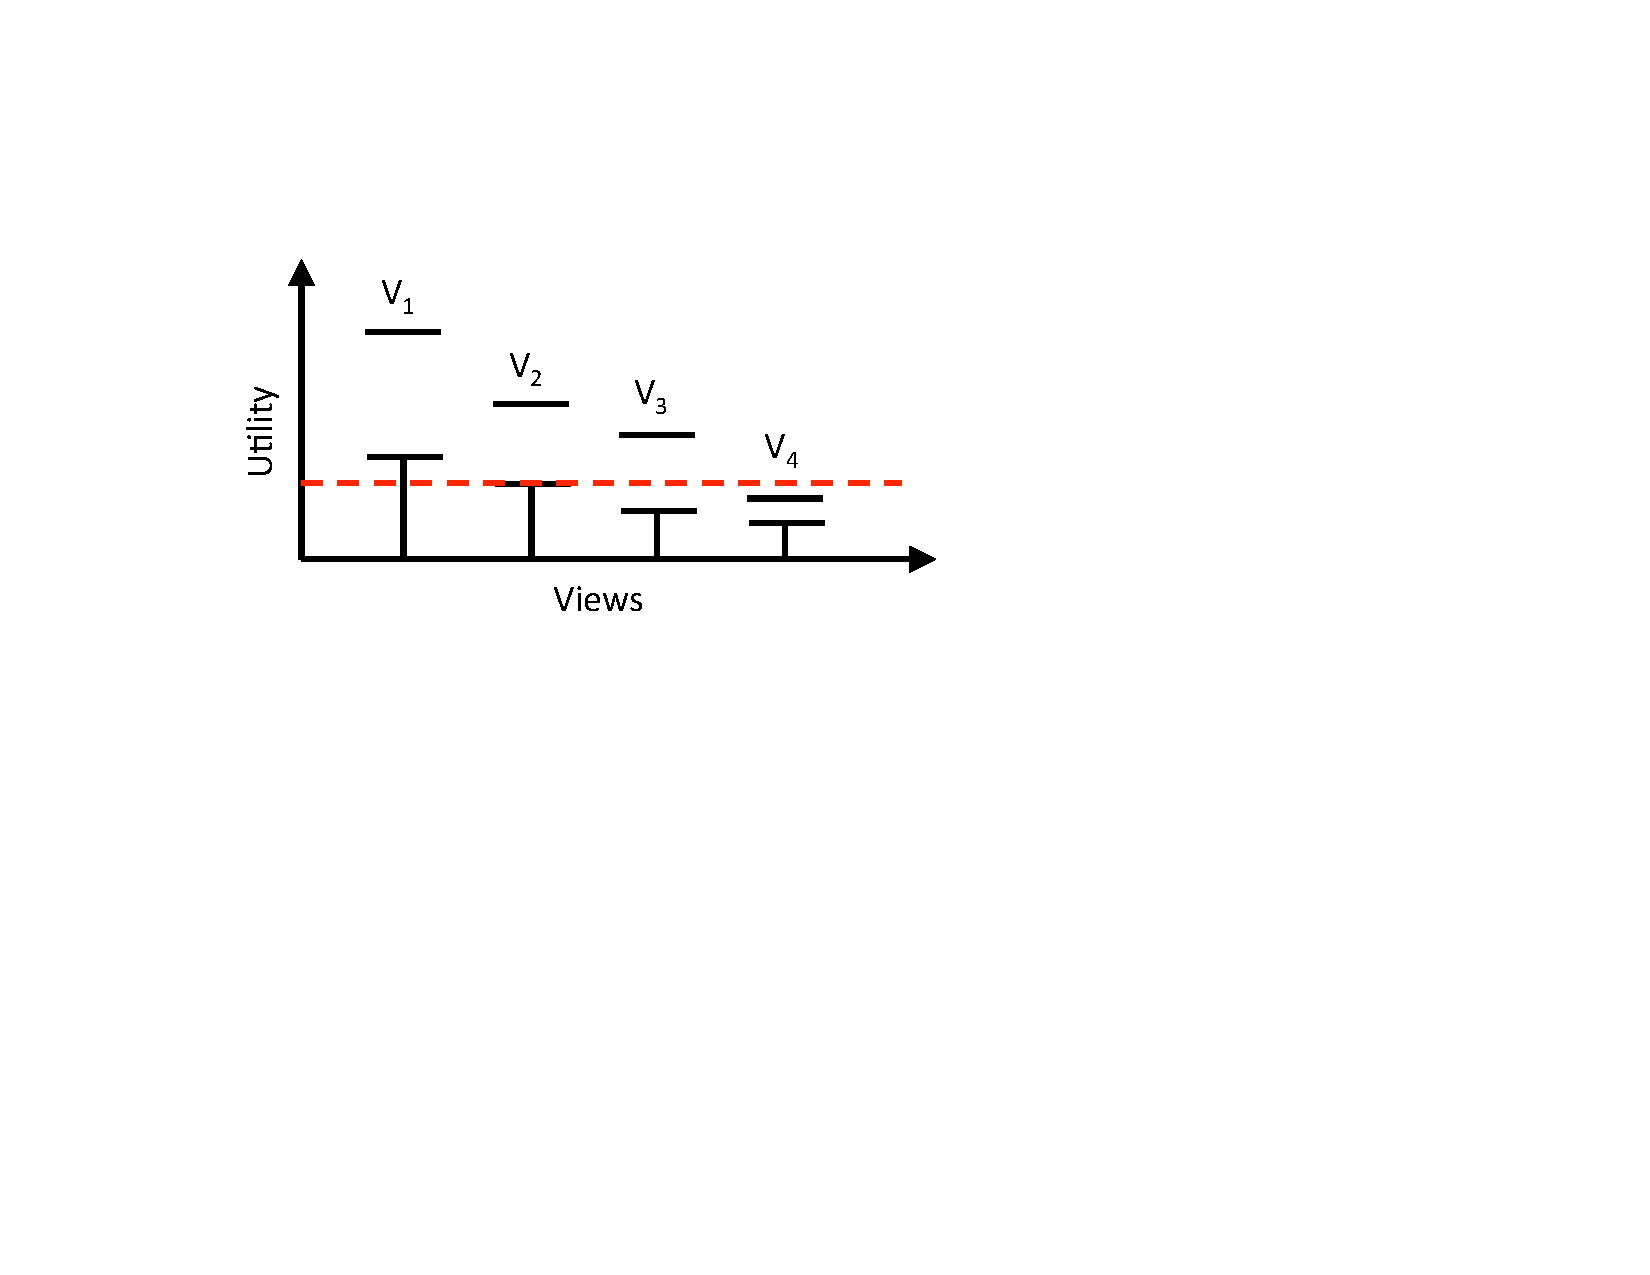
\includegraphics[trim=10mm 100mm 55mm 35mm, 
clip=true]{Images/confidence_pruning.pdf}}}}
\vspace{-20pt}
\caption{Confidence Interval based Pruning}
\label{fig:conf_interval}
\vspace{-12pt}
\end{figure}

Suppose at the end of phase $p$, confidence intervals for the views in
running have values shown in Figure \ref{fig:conf_interval} and we want to
identify the two views with the highest utility.
Views $V_1$ and $V_2$ have the highest utilities so far.
Consider view $V_3$; we see that its confidence interval overlaps with the
confidence intervals of the current top views $V_1$ and $V_2$, making it possible
that $V_3$ will be in the final top views. On the other hand, the confidence
interval for $V_4$ lies entirely below the lowerbounds of $V_1$ and $V_2$.
Since we can claim with high probability (depending on the confidence threshold)
that the utility of $V_4$ lies within its confidence interval, it follows that
with high probability, $V_4$'s utility will be lower than that of both $V_1$ and
$V_2$, and it will not appear in the top-$2$ views.
This is essentially our pruning rule. 

Next, we discuss the two techniques we support to compute confidence intervals.


\stitle{Worst-Case Confidence Intervals.} 
Suppose we have $N$ values $y_1, \ldots, y_n$ in $[0, 1]$, and we are drawing
from them without replacement. 
Say we have drawn $m$ values so far, which are $Y_1, \ldots, Y_m$.
Then, we use the Hoeffding-Serfling inequality~\cite{serfling1974probability} 
to derive a running 
confidence interval around the current mean 
of the $m$ values such that the actual mean of the $N$
is always within this confidence interval with a probability of $1 - \delta$:
\begin{theorem}
\label{thm:hs}
Let $\calY = y_1,$ $\ldots,$ $y_N$ be a set of $N$ 
values in $[0,1]$ with average value
$\frac1N \sum_{i=1}^N y_i = \mu$.
Let $Y_1,\ldots,Y_N$ be a 
sequence of random variables drawn from $\calY$ without
replacement.
Fix any $\delta > 0$. For $1 \le m \le N-1$, define
$$
\varepsilon_m = \sqrt{\frac{(1-\frac{m-1}N)(2\log \log (m) + \log(\pi^2/3\delta))}{2m}}.
$$
$$
\textrm{Then:} \ \   \Pr\left[ \exists m, 1 \le m \le N : 
  \left|\frac{\sum_{i=1}^m Y_i}{m} - \mu\right| > \varepsilon_m \right] 
\le \delta.
$$
\end{theorem}
In our setting, we treat the current mean, $\sum Y_i / m$ is the 
the current estimate of the utility of a view 
based on the entire set of records seen thus far that apply to that view. 
Therefore, to apply this pruning strategy, the only statistics
we need are the current estimate of the utilities.

Note that in this setting, we are assuming that since the
utility estimate at any stage of processing is in $[0, 1]$, 
the $Y_i$ values, i.e., the incremental contributions to the utility
that come from reading each record, are also between $[0, 1]$,
and are independent of the current value of the utility. 
This is is not true in our setting, 
because the utility function could be arbitrary.
Thus, the guarantees do not directly apply to our setting. 

\stitle{Normal Confidence Intervals.} In this scheme,
we apply the standard normal confidence intervals to our utility measurements
assuming that the underlying distribution is Gaussian.
% We describe the equations first assuming that
% when every time a record is read, for every view,
% a utility value is ``sampled''
% from a normal distribution. (This assumption is not
% quite correct; we will discuss this  below.)

Consider a specific view $V_i$. 
If the mean utility across the sampled records 
(i.e., the records read thus far) is $\mu$,
and the variance in the utility of the sampled records
is $\sigma$, then, we have:
\begin{align}
CI & = \mu \pm z \times \frac{\sigma}{\sqrt{m}}
\end{align}
Thus, the CI (or confidence interval) is 
a confidence interval centered around $\mu$, 
and depends on $\sigma$. 
It additionally depends on the number of records
read thus far, $m$,
and $z$, the factor that depends on our confidence interval threshold.
For instance, for a 95\% confidence interval, $z = 1.96$.

We note that the assumption that we are drawing from a normal distribution is
not quite accurate since our samples vary in size and are not independent.
As a result, we make two simple adjustments to the confidence interval
calculations that are described in Appendix \ref{}.
In Section \ref{}, we show experimentally on multiple datasets that our
confidence interval calculations accurately capture utility and can be used to
perform pruning with high confidence.






% \stitle{Normal Confidence Intervals.}
% As described above, we must specify
% a set of statistics to track for each view and a rule that is used to
% prune views based on the statistic.
% For confidence interval based pruning, the statistics we track are the mean, 
% variance, and confidence intervals of the view utility.
% As \VizRecDB\ reads each record, it updates the data
% distributions for all views and calculates the current utility of each view. 
% Using past measures of utility, \VizRecDB\ also tracks the mean,
% variance and confidence intervals for the utility of each view.
% % At the end of a phase, \VizRecDB\ uses the following rule for pruning low-utility
% % views (stated more formally below): {\it if the upperbound on the utility
% % of view $v_i$ is lesser than the least lowerbound on the utility of the
% % top-$k$ views, view $v_i$ is discarded.}

% % Let us dive deeper into this pruning rule.
% Note that as we sequentially read records from a file, we are
% approximating a sampling process (remember that the records are in random order).
% For instance, suppose that we have read 10K records from a 1M record file.
% In this case, the records 1 -- 10K constitute a 1\% sample of the entire file.
% When we read the next say 10 records, the records 1 -- 10,010 constitute an
% incrementally larger sample of the underlying file.
% Thus, as we read more data from the file, we obtaining a large
% number of samples from the underlying data (notice however, that these samples
% are not independent).

% Since we are generating a large number of samples from a population, we can
% invoke a well-studied concept in statistics called the ``sampling distribution.'' 
% A sampling distribution for a statistic $S$ is the distribution of
% $S$ generated by taking a large number of samples of a fixed size and computing
% the statistic $S$ on each sample.
% In our case, the population we draw from is the set of all records in the file
% and our samples are the increasingly larger sets of records that we are reading in.
% The statistic $S$ that we are computing is the view utility (we
% compute a utility value for each view).
% Now, the sampling distribution of the {\it mean} has been well studied and it
% has been proven that the mean of the sampling distribution is equal to the mean of the
% population and the standard error of the sampling distribution is equal to the
% standard error of the population divided by the square root of the sample size. 
% These two formulas are shown in Equations \ref{eq:mean} and \ref{eq:variance}.
% Similarly, if we know the mean and standard error of the sampling distribution,
% we can compute a confidence interval around the population mean. This is shown
% in Equation \ref{eq:confidence_interval} where $z$ is the factor that depends on the
% confidence threshold we are aiming for and $N$ is the number of items
% in each sample.

% \begin{eqnarray}
% \label{eqnarray:mean_and_variance}
% \mu_M = \mu \label{eq:mean}\\
% \sigma_{M} = \frac{\sigma}{\sqrt{N}} \label{eq:variance}\\
% CI = \mu_M \pm z \ast \frac{\sigma_M}{\sqrt{N}}\label{eq:confidence_interval}
% \end{eqnarray}

% If we were modeling the mean of our samples instead of the utility, we could use
% the above result directly.
% However, we find that with a few minor modifications, we can use the confidence
% interval bounds shown above.
% The first modification we make has to do with how we define utility.
% Remember from Section \ref{sec:problem_definition} that the utility of a view is
% defined as the distance between two distributions: the distribution of aggregate values for the
% target view and the distribution of aggregate values for the comparison view.
% These distributions are in turn tied to the number of distinct groups present in
% each dimension attribute.
% For our purposes, it means that if a dimension attribute has $n$ distinct
% groups, then a sample with $x$ rows gives us approximately $\frac{x}{n}$ values
% for each group (assuming uniform distribution).
% Said another way, a sample with $x$ rows for the purpose of computing utility is
% really only a sample of $\frac{x}{n}$ rows.
% So the first modification we make to Equation \ref{eq:confidence_interval} is to
% replace $N$ by $\frac{N}{G_{max}}$ where $G_{max}$ is the maximum number of
% distinct groups present in any dimension attribute.
% Second, we observe that the sampling distribution applies to the case where
% samples are of the same size and are independently generated.
% This is not true in our algorithm; therefore, to compensate, make two
% conservative modifications: we set $N$ to the number of rows that
% have been read in the previous phase (remember that pruning happens at the end
% of every phase) and we set the $z$ parameter to a value $\geq$ 1.96 (the normal
% 95\% confidence interval value). These modifications ensure (as we will show
% empirically in Section \ref{sec:experiments}) that the confidence intervals
% always contain the mean and continually shrink as we read in more data.

% As shown in Line 12 of Algorithm \ref{algo:custom_exec_engine},
% when a phase ends, we clear all statistics collected in that phase; we do not
% want less accurate estimates from previous phases to contaminate the more
% accurate estimates from subsequent phases. \agp{deal with this.}






% Now that we have a way of finding confidence intervals, we elaborate on how we
% use them to perfom pruning.
% Suppose at the end of phase $p$ the confidence intervals for the views in
% running have values shown in Figure \ref{fig:conf_interval} and we want to
% identify the two views with the highest utility.
% Consider view $V_3$, we see that its confidence interval overlaps with the
% confidence intervals of the current top views $V_1$ and $V_2$, making it likely
% that $V_3$ will be in the final top views. On the other hand, the confidence
% interval for $V_4$ lies entirely below the lowest bound of the top two
% intervals.
% Since we can claim with high probability (depending on the confidence threshold)
% that the utility of $V_4$ lies within its confidence interval, it follows that
% with high probability, $V_4$ will not appear in the top-$2$ views.
% This is essentially our pruning rule. 
% We state the algorithm fomally in
% Algorithm \ref{algo:ci_based_pruning}.

\begin{algorithm}
\caption{Confidence Interval Based Pruning}
\label{algo:ci_based_pruning}
\begin{algorithmic}[1]
\State viewsInRunning.sortByUpperbound()
\State topViews $\gets$ viewsInRunning.getTopK()
\State lowestLowerbound $\gets$ min(lowerbound(topViews))
\For {view $\not \in$ topViews}
\If {view.upperbound < lowestLowerbound}
\State viewsInRunning.remove(view)
\EndIf
\EndFor
\end{algorithmic}
\end{algorithm}

\subsubsection{Multi-Armed Bandit Pruning}
\label{sec:multi_armed_bandit}
The second class of pruning techniques we explore
are based on solutions for Multi-Armed Bandits (MAB), a problem 
in stochastic control. 
The setting is as follows: 
a gambler is faced with several slot
machines (``arms'') that each have an underlying reward
distribution. 
At each turn, the gambler must decide which machine
to play at; when they play the machine, they get a reward.
The gambler needs to decide on a {\em strategy}, i.e.,
which machine to play during every turn, to maximize
eventual, total, or time-decaying rewards~\cite{bandits}.
Recently, variants of MAB have been proposed 
which instead of maximizing total reward, 
focus on finding the bandits with the highest mean reward~\cite{BubeckWV13}.
This is very similar to our setting: each possible view can be thought of as
one arm and our goal is find the views with the highest reward (i.e.
utility).
In MAB, each pull of an arm corresponds to a drawing from a sample
the underlying probability distribution of that arm.
In our case, each new record updates the utilities for every possible view and
the every updated utility can be thought of as a sample from the underlying
utility distribution of that view.
There are two approximations we make here to apply the MAB techniques
to our setting
(as we show in our experimental evaluation,
the approximation works well
for our purposes.): 
(1) although the utility of a
view is ultimately a single value, we can approximate it as a probability
distribution that is normally distributed around the true utility, and 
(2) our running estimate of utility after reading $i$
records is an estimate derived from the above utility distribution.

Algorithm \ref{algo:mab_based_pruning} shows the pruning technique used in the
MAB setting.
This algorithm is an adaptation of Successive Accepts and Rejects
algorithm from \cite{BubeckWV13} for finding the top-$k$ arms with the highest
mean reward.
As before, the processing of the whole file is divided into phases.
% As opposed to the confidence interval technique, we only track a single
% statistic for MAB, namely the utility mean.
At the end of every phase, we adopt the following pruning technique: all views
in running are ranked in order of their utility means. 
We then compute two special differences between the utility means: $\Delta_1$
is the difference between the highest mean and the $k+1$st highest mean, and
$\Delta_n$ is the difference between the lowest mean and the $k$th highest mean.
If $\Delta_1$ is greater than $\Delta_n$, the view with the highest mean is
{\it accepted} as being part of the the top-$k$ (and it no longer participates
in pruning computations).
On the other hand, if $\Delta_n$ is higher, the view with the lowest mean is discarded
from the set of views in the running.


\begin{algorithm}
\caption{MAB Based Pruning}
\label{algo:mab_based_pruning}
\begin{algorithmic}[1]
\State viewsInRunning.sortByUtilityMean()
\State \{$\bar{u}_{i}$\} $\gets$ sorted utility means
\State $\Delta_1$ $\gets$ $\bar{u}_{1}$ - $\bar{u}_{k+1}$
\State $\Delta_n$ $\gets$ $\bar{u}_{k}$ - $\bar{u}_{n}$
\If {$\Delta_1$ < $\Delta_n$}
\State viewsInRunning.acceptTop()
\Else
\State viewsInRunning.discardBottom()
\EndIf
\end{algorithmic}
\end{algorithm}

% \techreport{\cite{BubeckWV13} provides bounds on the optimality of this heuristic for the
% MAB setting.
% Since our problem setup isn't exactly the same, the optimality bounds don't
% transfer directly.
% However, as we show in the experimental section, the MAB heuristic performs well
% on real datasets.}
 %!TEX root=document.tex

% \section{View Pruning}
% \label{sec:pruning}

\stitle{Offline Pruning.}
Even before any queries are issued to \SeeDB, we
have the ability to identify clusters of attributes
that are strongly correlated with each other, 
such that if we decide to select a visualization 
on one of them to display to the analyst, we can avoid 
displaying visualizations on others
(since they would be redundant).
Consider the following example using a hypothetical
dataset storing \agp{is this hypothetical?}
names of airports (as one attribute)
and airport codes (as another attribute).
Since names of airports and airport codes have
a 1:1 relationship, generating, say, 
average delay by airport name, and
average delay by airport code would lead
to identical visualizations. 
Consequently, it would suffice to compute and recommend
only one of these visualizations,
since the rest would contain redundant information.
\papertext{We describe how we perform
offline pruning, and describe the experimental
gains from offline pruning in our extended technical report.
At a high-level, we use clustering of attributes,
followed by clique detection to detect
and eliminate redundant aggregate views.}
View pruning allows us to significantly 
reduce the number of views (and execution time) in real
datasets; for the DIAB dataset described in Section \ref{sec:experiments},
we reduce the number of possible views from 72 to 41 (45\% reduction), and from
70 to 54 (25\% reduction) for the BANK dataset. 


% Intuitively, this pruning is important because fewer views equates to better
% performance.
% Note that the pruning performed by the view generator is based on redundancy while that performed by the execution engine is based on low utility.
% We distinguish between the pruning performed by the execution engine and the pruning
% performed by the view generator: the execution engine prunes {\it low-utility} views
% while the view generator prunes {\it redundant} views. 
% A set of views $\{V\}$ is said to be redundant if all views in $\{V\}$ have
% similar distributions and are therefore expected to have similar utility.
% For instance, consider a hypothetical dataset that stores the names of airports along
% with the corresponding airport code. 
% Views produced by grouping along either of these attributes will be identical.
% Similarly, Figure \ref{} shows three views of a real-world dataset (the DIAB dataset 
% from Section \ref{sec:experiments}).
% We observe that these views are very similar and hence it would suffice to compute
% and recommend only a representative view (while noting similar views).

% An extreme example of redundant views is the following: a table stores the sales
% of a product as measured in US Dollars and measured in Euros. 
% Views with either of these column as the measure attribute will be identical and
% have the same utility.
% Similarly, if a table has two dimension attributes, one corresponding to the
% airport name and another corresponding to the airport code, views with either
% of these attributes as dimensions are guaranteed to produce identical views.
% In both of the above cases, it suffices to compute and show a single view
% that is representative of multiple views (and list redundant
% views that have been omitted).
\techreport{
\agp{this needs fixing but probably more immediate things
need fixing as well.}
We adopt the following steps to prune redundant views: 
(1) For each table, the we first use the metadata about
attributes to determine the entire space of aggregate views. 
(2) We first prune all aggregate views containing attributes with 0 or low variance since
corresponding visualizations are unlikely to be interesting.
(3) For each remaining view $V_i$, it computes the distribution 
$P[V_i (D)]$ for the comparison view.
The resulting distributions are then clustered based on pairwise
correlation.
(4) From each cluster, the view generator picks one view to compute as a cluster representative and stores the clustered views compactly for subsequent use.
At run time, the view generator accesses previously generated view stubs, removes any views that would be redundant given
the input query (e.g. views grouping by state when the query only selects records
with \'state=``MA''\') and passes the remaining stubs to the execution engine.
\agp{Also, would be good to have some experimental figures or more details on this}
}


% We next compute pairwise correlations between these vectors (note: correlation is
% only defined for equi-sized vectors) and cluster views based on this correlation.
% Views in each cluster are expected to produce views with very similar distributions
% and therefore utilities.
% As a result, we pick only a single view from every cluster.
% Stubs corresponding to the selected views are stored compactly on disk for subsequent use.


% Next it computes the correlation between distributions corresponding to each
% pair of views (note that the dimensions must have same cardinality for this
% comparison to be valid).
% Correlation scores are thresholded and used to cluster views into groups.
% Finally, we pick a single view from every view cluster.


% Details of our pruning algorithm are presented in Appendix
% \ref{sec:view_pruning} along with examples of view clusters.


% In this section, we discuss an important component of \SeeDB\ that is invoked
% even before the Execution Engine runs, namely the View Generator.
% Given a user query $Q$, the purpose of the view generator module is to take the
% input query, obtain metadata about the underlying tables and use correlations
% between different columns in the table to prune views whose evaluation is
% unnecessary. 
% We distinguish between the pruning done in the execution engine and the pruning
% done in the view generator: the execution engine prunes away low-utility views
% while the view generator prunes away {\it redundant} views.
% So what are redundant views? Redundant views are views that have similar
% distributions and are therefore expected to have similar utility.
% An extreme example is that of sales of a product as measured in US
% Dollars and measured in Euros. Views with these measure attributes will be
% identical and have the same utility.
% Similarly, two dimension attributes, one corresponding to the airport name
% and another corresponding to the airport code are guaranteed to produce identical
% views irrespective of the measure attribute.
% In both of the above cases, it suffices to compute and show only a single view
% that is representative of multiple views (the frontend does list redundant
% views that have been omitted).

% The View Generator works in two stages: it performs view pruning offline and
% identifies the set of viable views; then, when a new user query comes in, it
% reads the set of viable views, performs pruning based on the input query and
% passes view stubs on to the Execution Engine. 
% The offline pruning does not depend on the input query and can therefore be
% perfomed only once.
% The offline stage works as follows. 

% First, for each table, the View Generator obtains various types of
% metadata including the data types of attributes, their classification into
% measure and dimension attributes, number of distinct values for dimension
% attributes, and the distributions for each measure attribute (mean, std
% deviation).
% The first piece of metadata is essential to determine the full space of
% views. 
% The number of distinct values for dimension attributes and the variance for
% measure attributes is used to perform basic pruning of views (e.g. views
% containing zero variance attributes will have low utility).

% \mpv{If two dimension attributes $a_i$ and $a_j$ have
% a high degree of correlation (e.g. full name of airport and abbreviated name of
% airport), the views generated by grouping the table on $a_i$ and $a_j$ will be
% very similar (and have almost equal utility). We can therefore generate and
% evaluate a single view representing both $a_i$ and $a_j$. \SeeDB\ clusters
% attributes based on correlation and evaluates a representative view per
% cluster.}



  
% We next describe a scheme that allows us to associate upper and lower bounds for
% views by evaluating them on a small sample of the dataset.
% We describe the use of the scheme on a simple view where AVG(Y) for a given
% attribute Y is being computed for each group in attribute X.
% We can then depict this view using a bar chart or a histogram.
% 
% For this derivation, we assume that the AVG(Y) for any X = $x_i$, is normally
% distributed around a certain mean $p$.
% Given a number of samples for Y for X = $x_i$, we can employ the following
% theorem \cite{stats_book} to bound $p$ within a confidence interval with
% probability $1 - \delta$:
% \begin{theorem}~\label{thm:confint}
% If $\hat{p}$ and $s$ are the mean and standard deviation 
% of a random sample of size $n$ from a normal distribution with unknown 
% variance, a $1 - \delta$ probability confidence interval
% on $p$ is given by:
% $$\hat{p} - \frac{t_{\delta/2, n-1} s}{\sqrt{n}} \leq p \leq \hat{p} + \frac{t_{\delta/2, n-1} s}{\sqrt{n}}$$
% where $t_{\delta/2, n-1}$ is the upper 100$\alpha/2$ percentage point
% of the $t$-distribution with $n-1$ degrees of freedom.
% \end{theorem}
% 
% Now, we demonstrate how we can use this theorem to establish an upper 
% and lower bound for the utility of a view, with probability $1 - \delta$.
% 
% Let the distance vector corresponding to the target view be:
% $\bar{a} = [a_1, a_2, \ldots, a_k]$ while the distance vector corresponding to
% the comparison view is:
% $\bar{b} = [b_1, b_2, \ldots, b_k]$.
% Notice that on very large datasets, it may be beneficial to precompute the
% distance vectors corresponding to the comparison views, so we assume that the
% vector $\bar{b}$ is computed exactly and known in advance.
% We let $a = \sum_i a_i$, and $ b = \sum_i b_i$.
% 
% Our goal is to use the sample to bound the values of the $a_i$ around $\ha_i$
% such that we can establish upper and lower bounds for the utilities.
% By applying Theorem~\ref{thm:confint}, we
% can get values $c_i$ for which $a_i \in [\ha_i - c_i, \ha_i + c_i]$
% with probability greater than $1 - \delta/k$.
% (By union bound, we will be able to ensure that all $a_i$'s
% are in their intervals with probability $1 - \delta$.)
% 
% Now, given these values $c_i$, we can establish an upper bound for the
% EMD (and also similarly for other distance metrics) in the following manner:
% We let $q_1(\bar{a}) = \sum_i \ha_i - c_i$, and $q_2(\bar{a}) = \sum_i \ha_i + c_i$.
% 
% 
% \begin{align*}
% EMD(\bar{a}, \bar{b}) & = \sum_i |a_i / a - b_i / b|\\
%           & = \sum_i |a_i / a - b_i / b|\\
%           & = 1/ab \sum_i \max (a_ib  - b_ia, b_ia - a_ib)\\
% \end{align*}
% Thus, we have:
% \begin{align}
% \frac{1}{b q_1(\bar{a})} \sum_i \max (a_ib  - b_ia, b_ia - a_ib) \leq & EMD(\bar{a}, \bar{b}) \leq \frac{1}{b q_2(\bar{a})} \sum_i \max (a_ib  - b_ia, b_ia - a_ib)\label{eq:emd}
% \end{align}
% 
% Note that: 
% \begin{align*}
% (\ha_i - c_i)b  - b_i (\sum_i (\ha_i + c_i)) & \leq a_ib  - b_ia  \leq (\ha_i + c_i)b  - b_i (\sum_i (\ha_i - c_i)), \textrm{\ and} \\
% b_i (\sum_i (\ha_i - c_i)) - (\ha_i + c_i) b & \leq b_i a  - a_i b  \leq  b_i (\sum_i (\ha_i + c_i)) - (\ha_i - c_i) b
% \end{align*}
% By plugging these quantities back into Eq~\ref{eq:emd},
% we have upper and lower bounds on the EMD metric.
% Similar mechanisms may be used to derive upper and lower bounds for other metrics.
% 
% Now that we have upper and lower bounds for the utility of each target view
% by evaluating the query on a sample,
% we can easily use it to prune away a number of views that are definitely not likely to be part 
% of the top-K,
% and instead focus on views that may be part of the top-K.

%   \subsection {Partitioning Tables}
%   The increase in the total execution time when a large number of queries are
%   executed in parallel suggests that there is a ``sweet spot'' with respect to
%   the maximum number of queries that can be run in parallel on a given table.
%   Therefore, we uniformly partition large tables into smaller ones and run
%   subsets of queries against each of the partitions. Note that the views
%   returned are nor approximate because we are now executing views against
%   subsets of the data. As a result, bounds developed in sampling now apply. We

 


%If a dimension attribute $\mathcal{d}$ is highly correlated with measure
  %attribute $\mathcal{m}$, then?

% \mpv{also from full paper draft}
% It is possible to collect the above statistics at the dataset level too, as
% opposed to the entire table level. The advantage of table level statistics is
% that they have to be computed only once per table; however, dataset-level
% statistics are more accurate since they only consider the specific parts of the
% table. XXX: we use dataset-level statistics with table statistics do not result
% in aggressive pruning. 




 \section{Experimental Evaluation}
\label{sec:experiments}
 
In this section we present an experimental evaluation of \VizRecDB, using
 both real and synthetic datasets to investigate performance of \VizRecDB.
Our goals were the following: (a) to study the performance characteristics of
the DBMS-backed execution engine and the custom execution engine, (b) to study the
accuracy of the heuristics developed in Section \ref{}, and (c) to test how well
\VizRecDB\ performs on real datasets. 
We use the datasets listed in Table
\ref{tab:datasets} to study various properties of out techniques.

\begin{table}[htb]
  \centering \scriptsize
  \begin{tabular}{|c|c|c|c|c|c|} \hline
  Name & Description & Size & Dims & Measures & Views \\ \hline
  SYN1 & Synthetic data & 1M & 50 & 5 & 250 \\
  & Randomly distributed, & & & & \\ 
  & varying \# distinct values & & & & \\ \hline
  SYN2 & Synthetic data & 1M & 50 & 20 & 1000 \\
  & Randomly distributed, & & & & \\ 
  & varying \# distinct values & & & & \\ \hline
  SYN3-10 & Synthetic data & 1M & 20 & 1 & 20 \\
  & Randomly distributed, & & & & \\ 
  & 10 distinct values/dim & & & & \\ \hline
  SYN3-100 & Synthetic data & 1M & 20 & 1 & 20 \\
  & Randomly distributed, & & & & \\ 
  & 100 distinct values/dim & & & & \\ \hline
  BANK  & Customer Loan dataset  & 40K & 10 & 8 & 80* \\ \hline
  DIAB  & Hospital data & 100K & 10 & 8 & 80* \\
  & about diabetic patients & & & & \\ \hline
  \end{tabular}
  \caption{Datasets used for testing}
  \label{tab:datasets} 
\end{table}

In the sections that follow, we show experimental results demonstrating that:
(a) Our optimizations to \VizRecDB's DBMS-backed engine can reduce latency by
50XX from 500s to 10s for the row store and from XXX to YYY for the column
store.
(b) Column stores are much well suited to the \VizRecDB\ workload and perform XXX times
faster on average than row stores. 
(c) Our pruning heuristics produce results with XXX accuracy for multiple real
world datasets.
(d) Our pruning heuristics can reduce latency by upto 90\% without taking a
significant hit in accuracy.
We begin with an evaluation of the DBMS-backed execution engine followed by an
evaluation of our custom solution.

 All experiments were run on a single machine with 8 GB RAM and a 16 core Intel
 Xeon E5530 processor. 

\subsection{DBMS-backed Execution Engine}
\label{sec:expts_dbms_execution_engine}

% As mentioned in Section \ref{sec:dbms_execution_engine}, our DBMS-based
% execution engine leverages the DBMS API to execute view queries directly on the
% database.
% While this approach has the advantages of reusing existing query procesing
% systems and being agnostic to the specific underlying DBMS, its limitations
% include the lack of fine grained control over sharing of table scans and lack of
% ability to prune low-utility views. 
In our first set of experiments, we investiage how well our DBMS-backed engine
can support a \VizRecDB-style workload, and how the optimizations
presented in Section~\ref{XXX} perform.
The key metric we are concerned is latency -- what was the total time taken by
\VizRecDB\ to compute the top views for any given query.
All experiments were repeated three times and the latency measures were
averaged.
Since this version of the execution engine exhaustively explores all views and
 orders them by utility, we are guaranteed to get the top-$k$ views with
perfect accuracy.
We ran all our experiments in this section on two database systems: a
row-oriented database (denoted as ROW in the following figures) and a
column-oriented database (COL).
The reason for evaluating both systems was that we expect (and
demonstrate below) that certain optimizations to work better for row-stores vs.
column stores.
Moreover, we show that column stores are better suited for a \VizRecDB\ style
workload.

The following experiments use synthetic datasets SYN1, SYN2, SYN3-10 and
SYN3-100. 
We chose to test our optimizations on these datasets since we could
control all aspects of the data including size, number of
dimensions and measures, data distribution and number of distinct values.
After studying the effect of our optimizations on synthetic data, we report the
results of running our techniques on the real datasets BANK and DIAB.
We start with an evaluation of the basic framework and
then study the effect of adding each individual optimization. \\

\noindent {\it Basic Framework}: The basic DBMS-backed execution engine
serially executes individual view queries, two for each possible view.
Figures \ref{fig:baseline_size} and \ref{fig:baseline_views} show
\VizRecDB\ latency when using the basic framework.
For these experiments, we used the SYN dataset and created subsets of SYN  with
varying number of rows and views (by varying number of dimension attributes). 
In
Figure \ref{fig:baseline_size} we show the latency of \VizRecDB\ as a function
of the number of rows (100K rows -- 1M rows) in the dataset and in 
 \ref{fig:baseline_views} 
we show the latency as a function of the number of possible views
(50 to 250).
We can make a few observations from these charts. First, the basic framework has
very poor performance: the row store takes between 50-500s to run the \VizRecDB\ queries
while the column store takes 10-100s. These time scales are not practical for
any interactive applications. Second, column stores run about 5X faster than row
stores for this workload. 
This is expected because individual view queries only select one dimension
attribute and one measure attribute at a time.  The column store can just read these two
columns, whereas the row-store must read all data from each table.
Third, as expected, the latency of the
basic framework is directly proportional to the number of rows as well as the 
number of views in the table.

Since the latencies for the basic framework are very high for interactive
applications, it is clear that we must aggressively optimize our queries. \\

% \begin{figure}[h] 
% \centerline{
% \resizebox{4cm}{!} {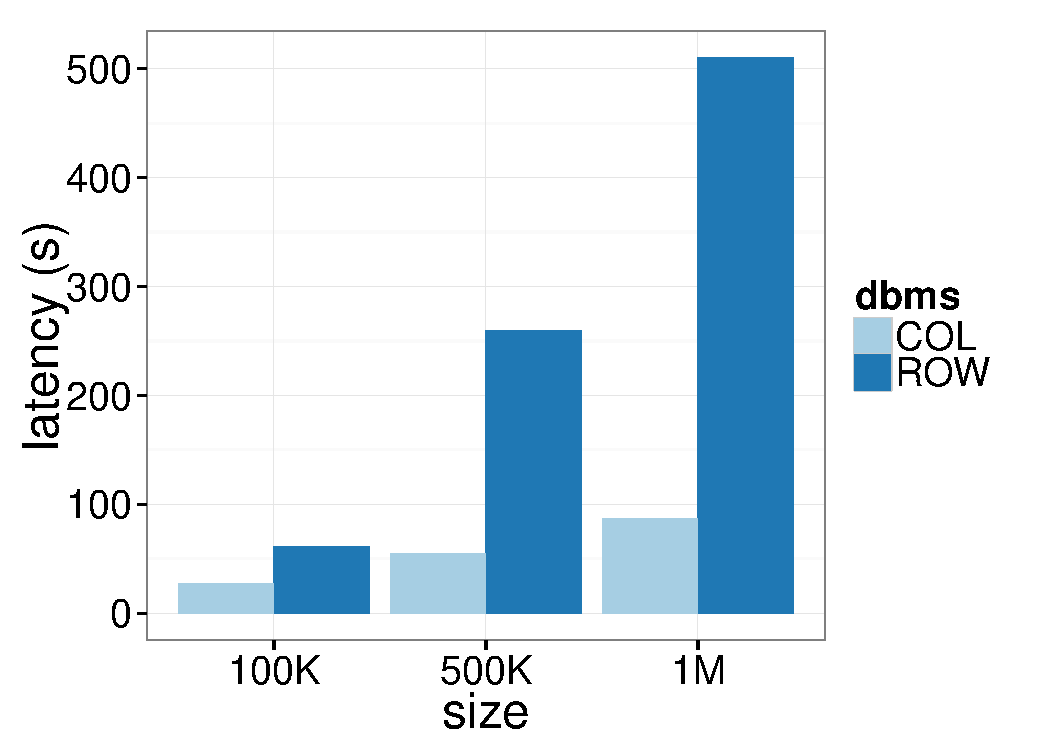
\includegraphics {Images/baselines_by_size.pdf}}
% \resizebox{4cm}{!} {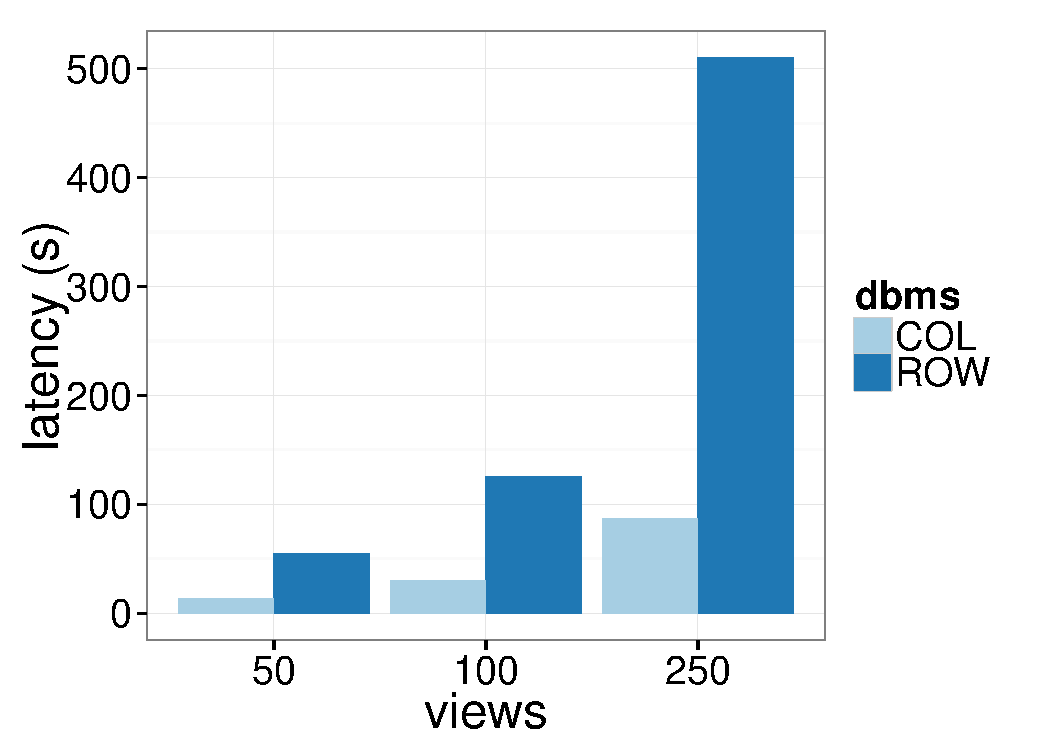
\includegraphics {Images/baselines_by_views.pdf}}
% }
% \end{figure}

\begin{figure*}[t]
	\centering
	\begin{subfigure}{0.33\linewidth}
		{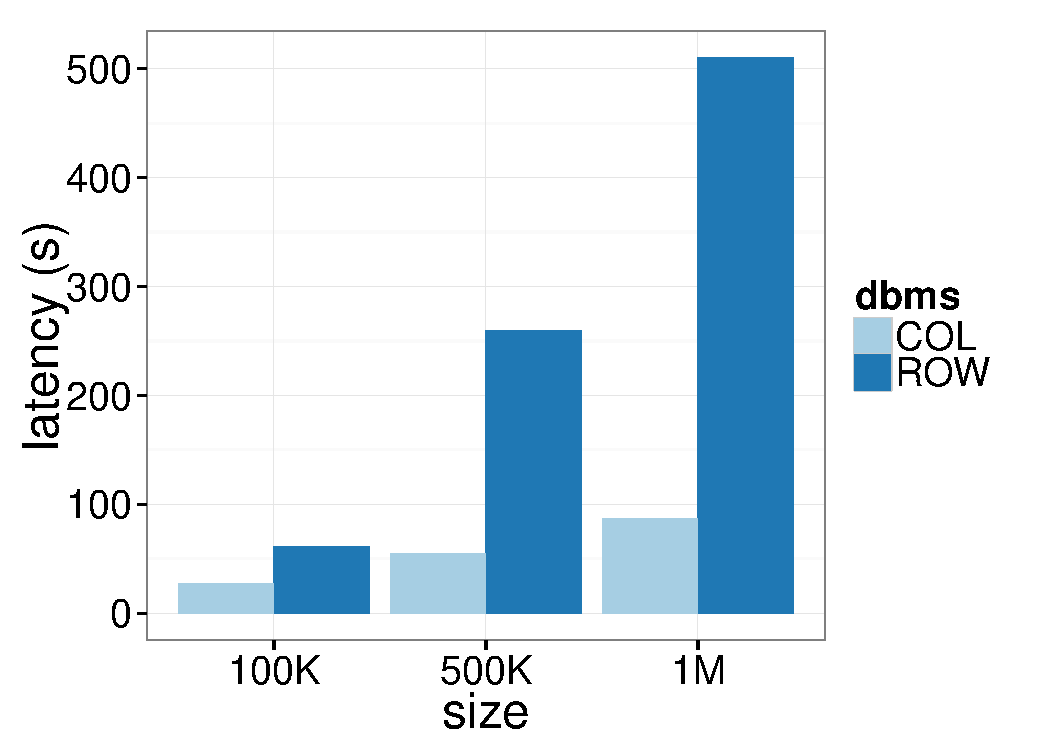
\includegraphics[width=6cm] {Images/baselines_by_size.pdf}}
		\caption{Latency vs. Table size}
		\label{fig:baseline_size}
	\end{subfigure}
	\begin{subfigure}{0.33\linewidth}
		\centering
		{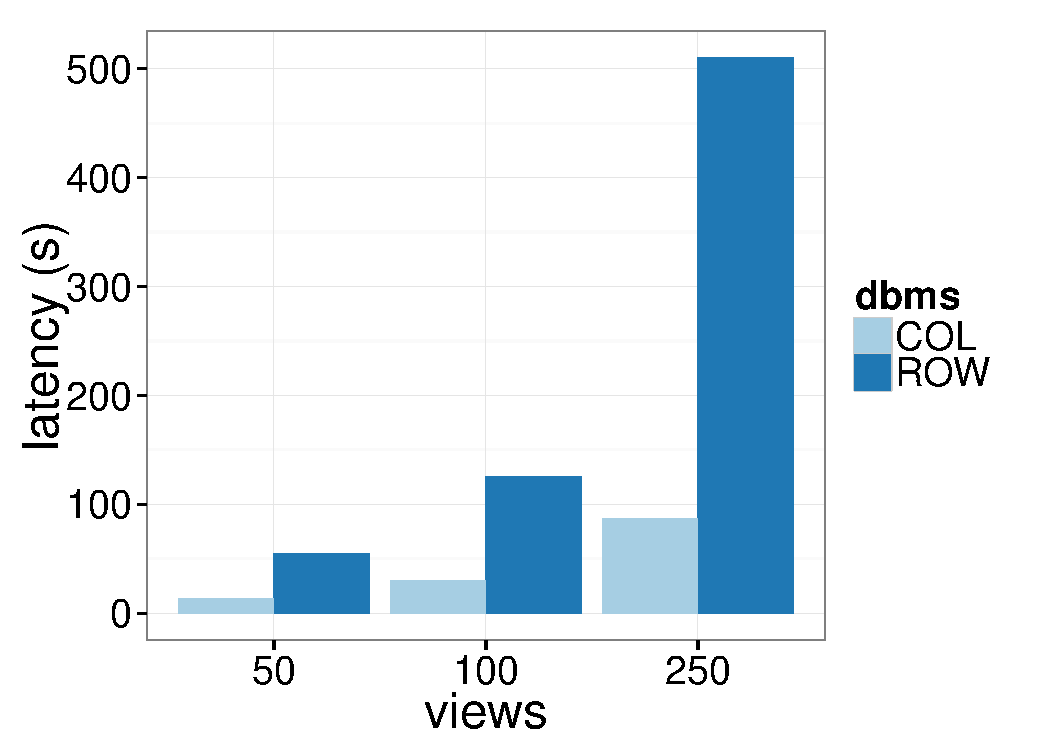
\includegraphics[width=6cm] {Images/baselines_by_views.pdf}}
		\caption{Latency vs. Num Views}
		\label{fig:baseline_views}
	\end{subfigure}
	\begin{subfigure}{0.33\linewidth}
		{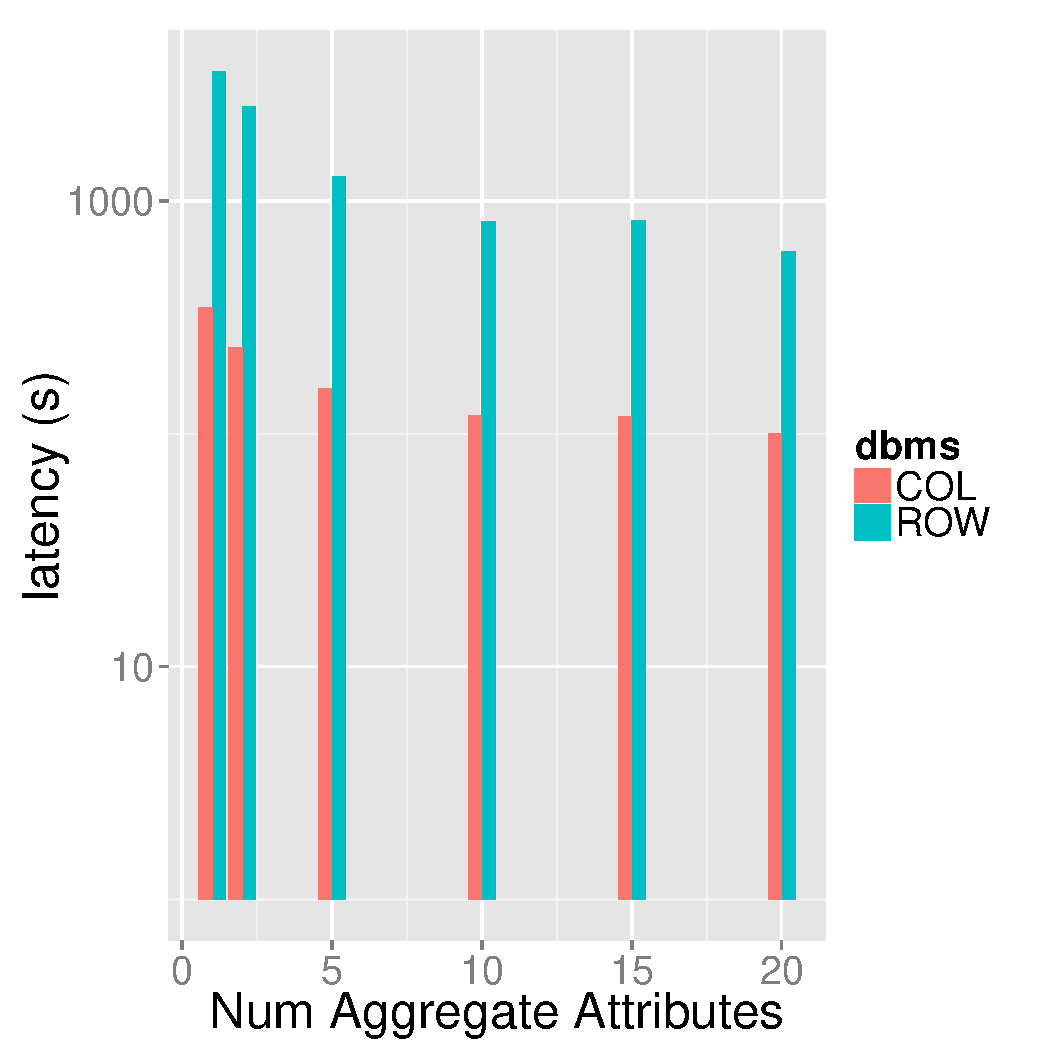
\includegraphics[width=6cm] {Images/multi_agg.pdf}}
		\caption{Latency vs. number of aggregates}
		\label{fig:multi_agg}
	\end{subfigure}
	\caption{Baseline performance and Effect of Parallel Query Execution \srm{I am not a fan of the gray backgrounds here; use white.  Also us more contrasty colors and ensure it prints OK in black and white.  Finally, lines in line plots should be thicker.  Also, why are we using bars for size/views and lines for number of queries.  Be consistent (just use bars -- easier to read.)}}
	\label{fig:bank_perf}
\end{figure*}

\begin{figure*}[t]
	\centering
	\begin{subfigure}{0.33\linewidth}
		\centering
		{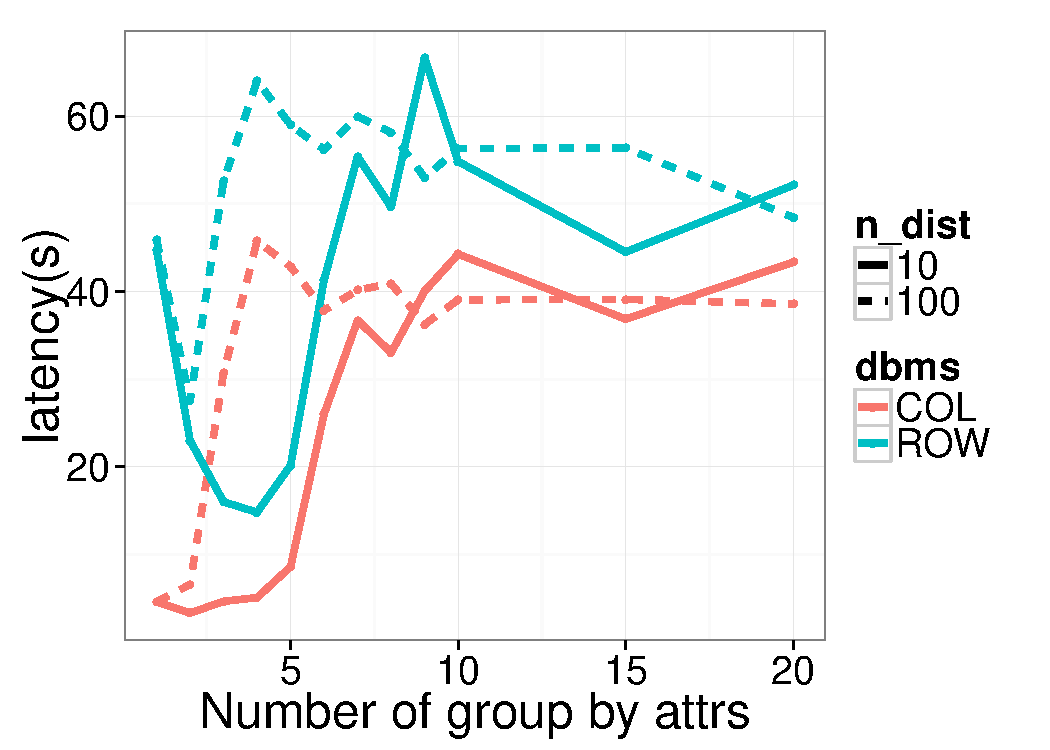
\includegraphics[width=6cm] {Images/multi_gb_same.pdf}}
		\caption{Latency vs. Num of Groups}
		\label{fig:multi_gb_same}
	\end{subfigure}
	\begin{subfigure}{0.33\linewidth}
		\centering
		{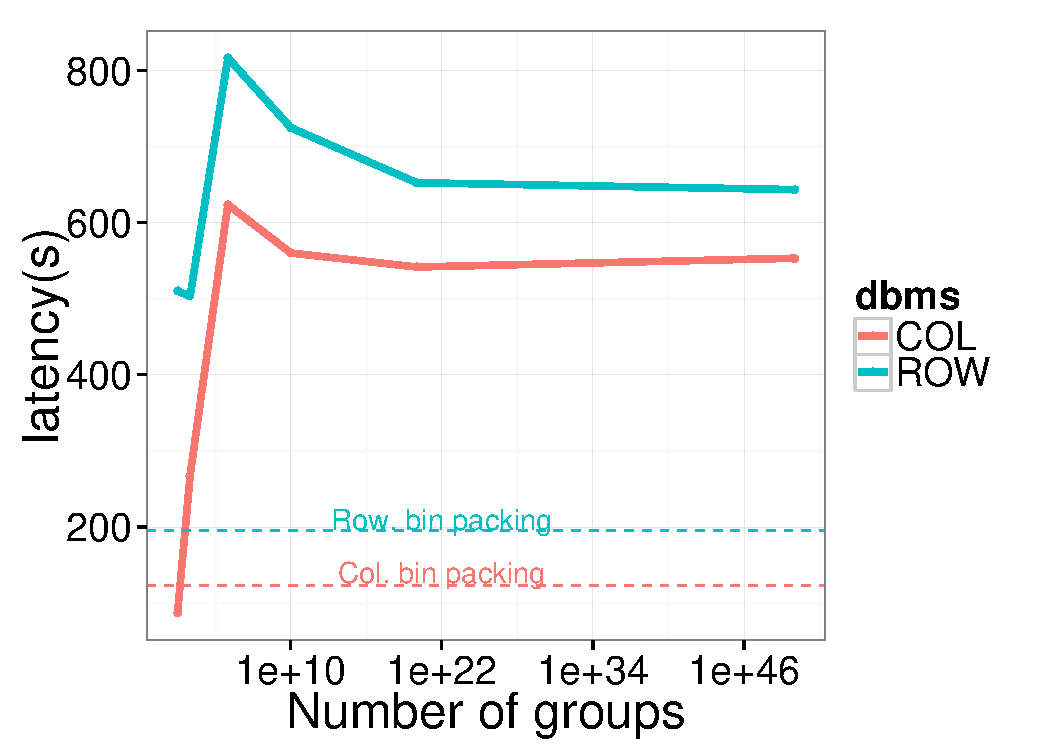
\includegraphics[width=6cm] {Images/multi_gb.pdf}}
		\caption{Latency vs. Num Dimensions}
		\label{fig:multi_gb_bp}
	\end{subfigure}
	\begin{subfigure}{0.33\linewidth}
		\centering
		{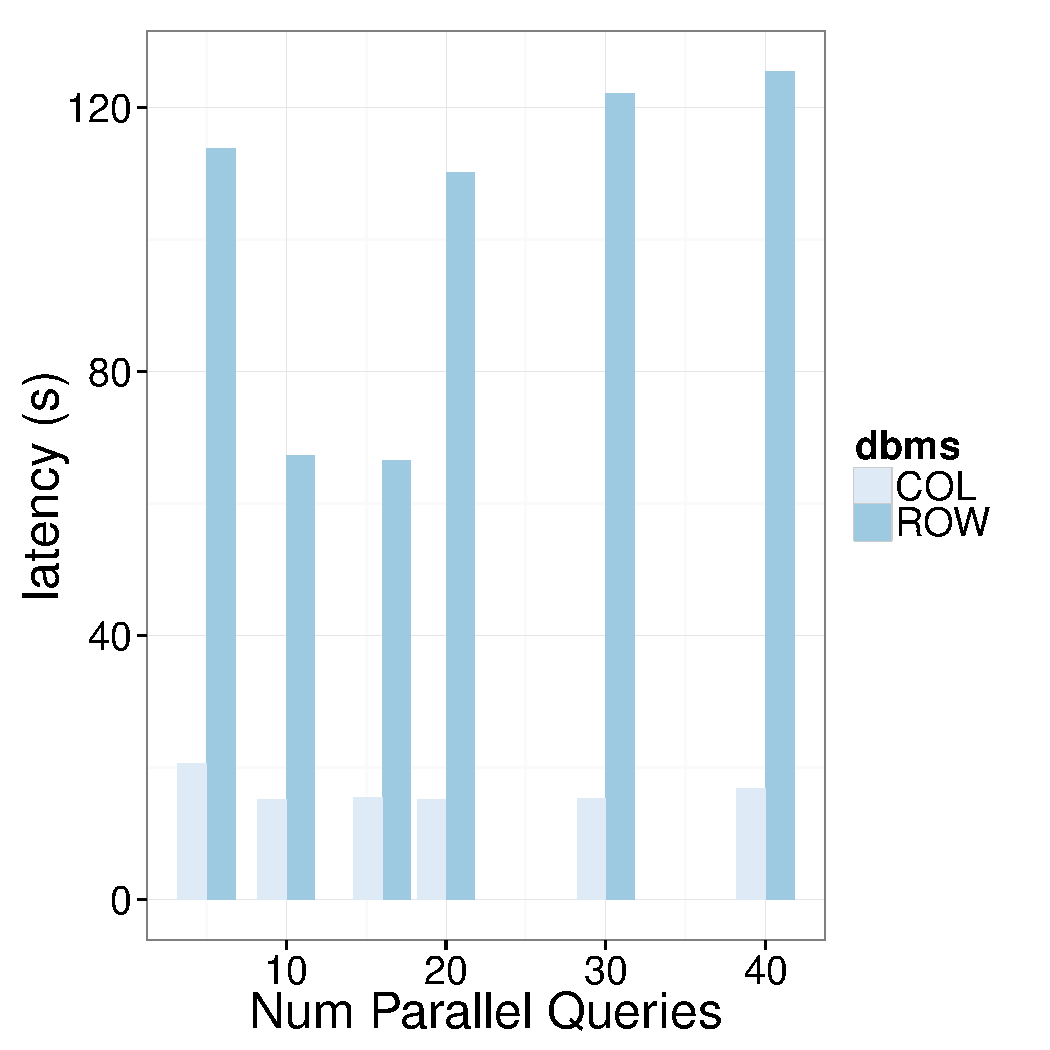
\includegraphics[width=6cm] {Images/parallel_noop.pdf}}
		\caption{Effect of parallelism}
		\label{fig:parallelism}
	\end{subfigure}
	\caption{Effect of Combining Multiple Queries \srm{Need to add a legend or mark on the figure indicating that the dotted lines are the bin packing heuristic.}}
	\label{fig:bank_perf}
\end{figure*}

\begin{figure*}[t]
	\centering
	\begin{subfigure}{0.24\linewidth}
		\centering
		{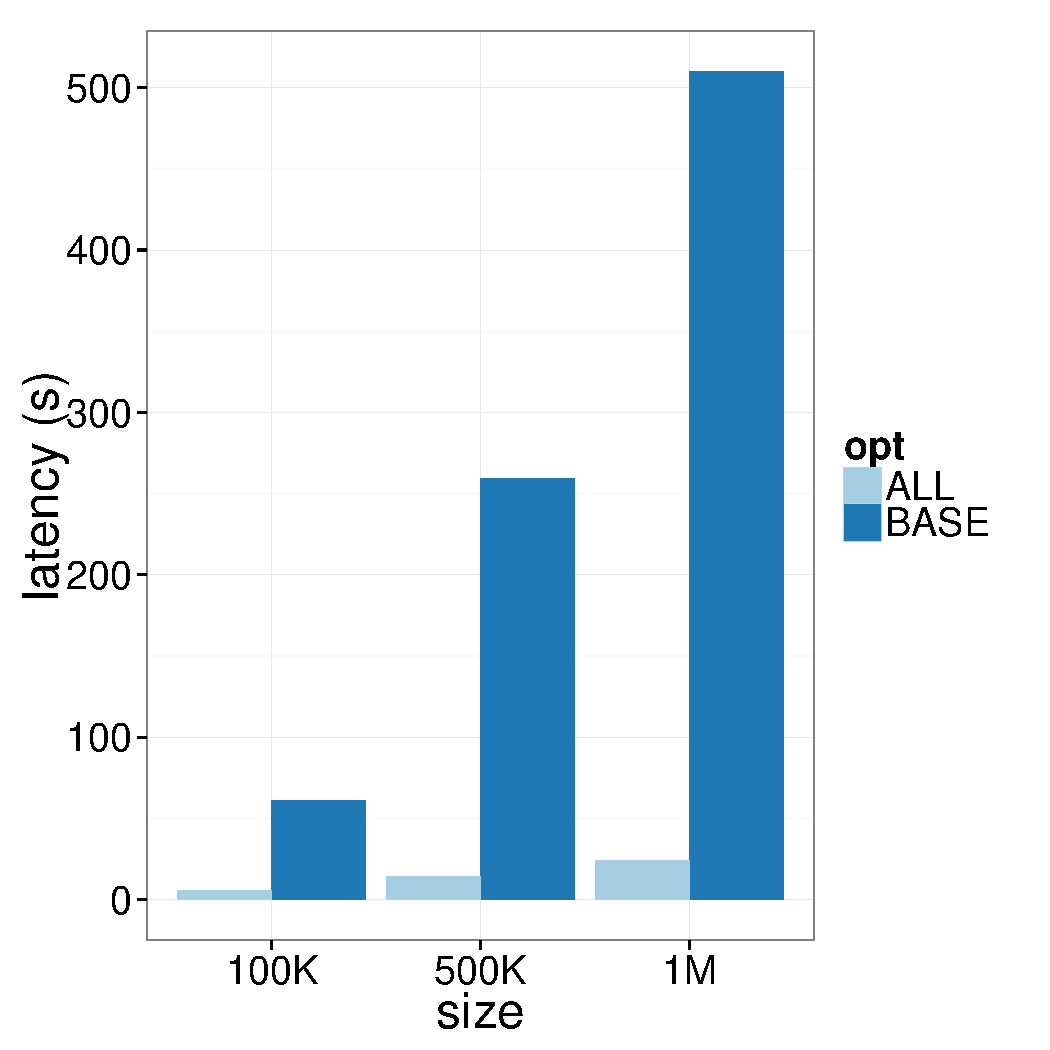
\includegraphics[width=4.6cm] {Images/row_all_none_by_size.pdf}}
		\caption{Row store latencies by Size}
		\label{fig:row_all_none_size}
	\end{subfigure}
	\begin{subfigure}{0.24\linewidth}
		\centering
		{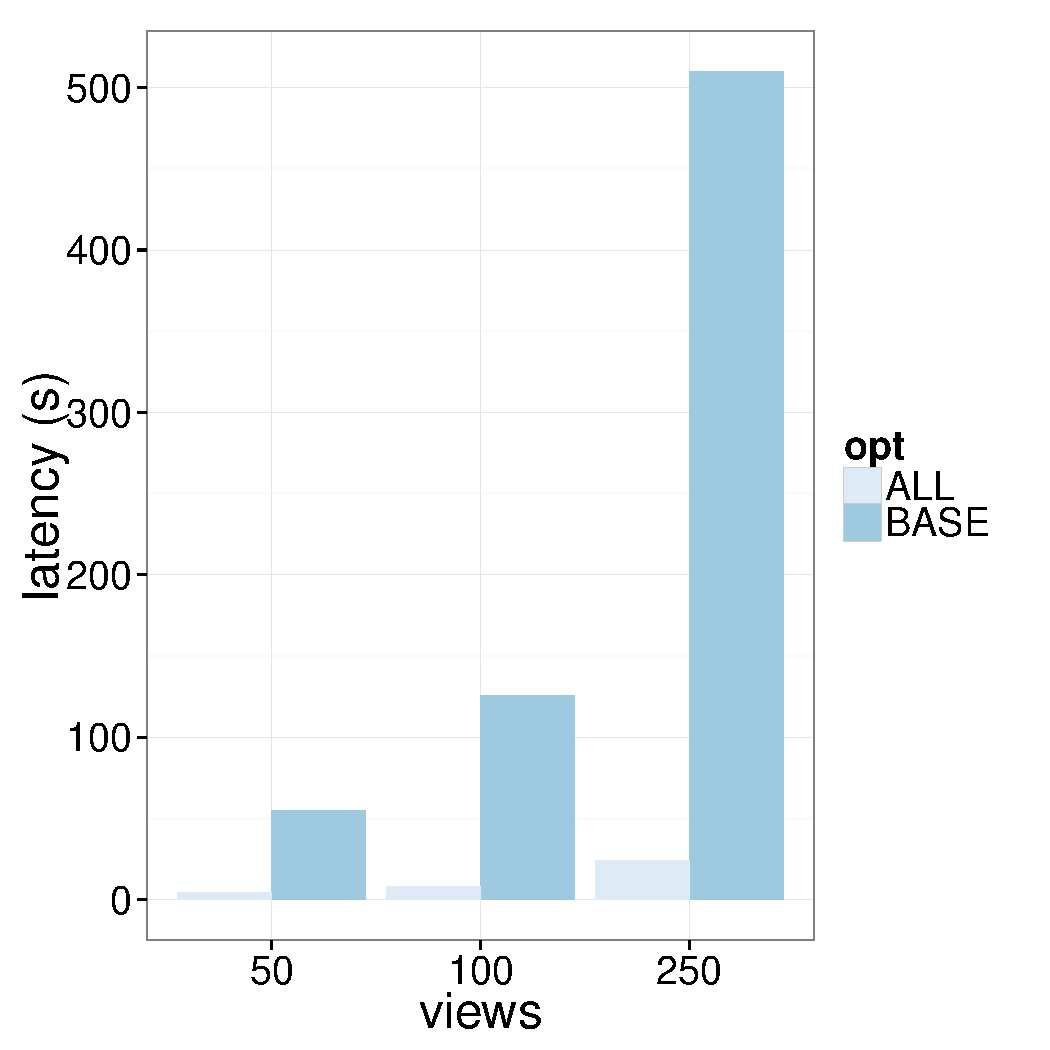
\includegraphics[width=4.6cm] {Images/row_all_none_by_views.pdf}}
		\caption{Row store latencies by Views}
		\label{fig:row_all_none_views}
	\end{subfigure}
	\begin{subfigure}{0.24\linewidth}
		\centering
		{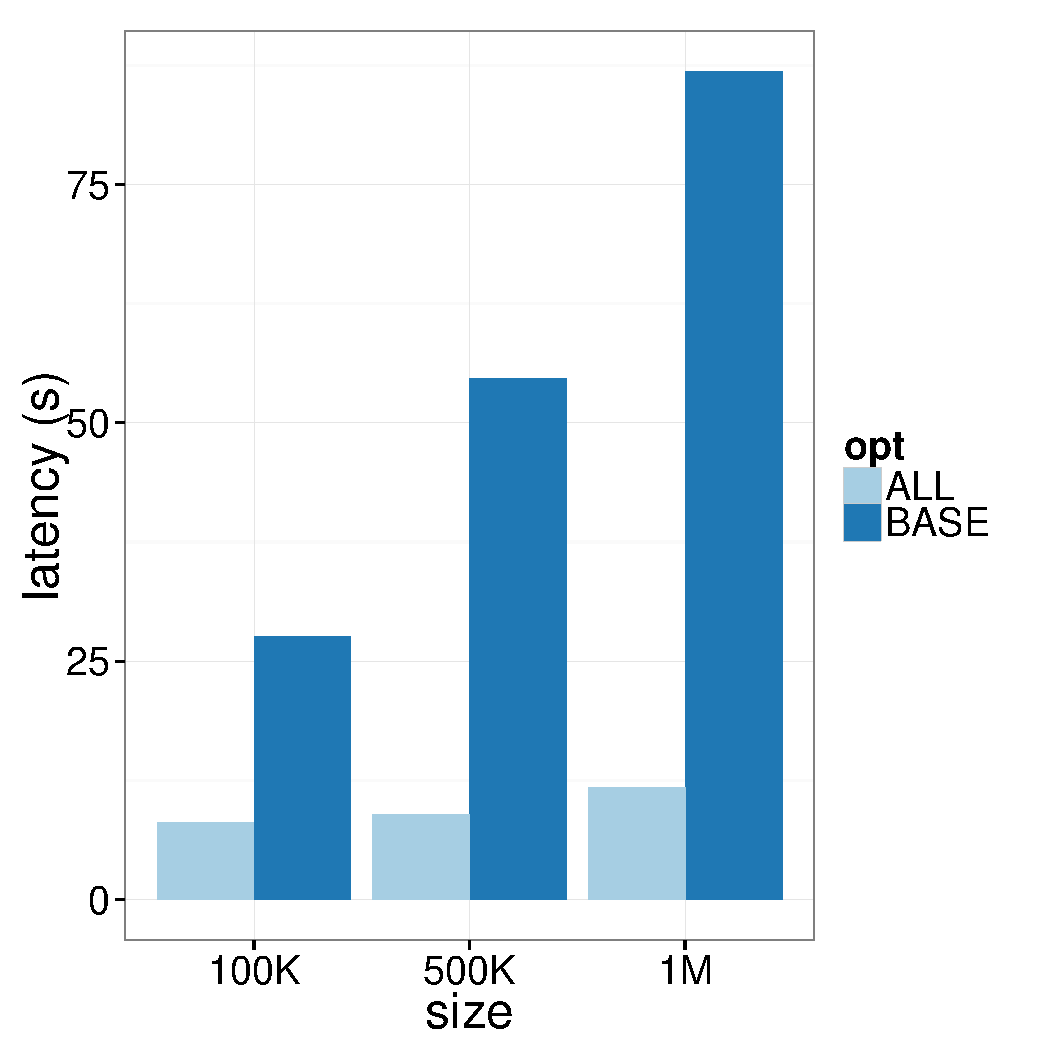
\includegraphics[width=4.6cm] {Images/col_all_none_by_size.pdf}}
		\caption{Column store latencies by Size}
		\label{fig:col_all_none_size}
	\end{subfigure}
	\begin{subfigure}{0.24\linewidth}
		\centering
		{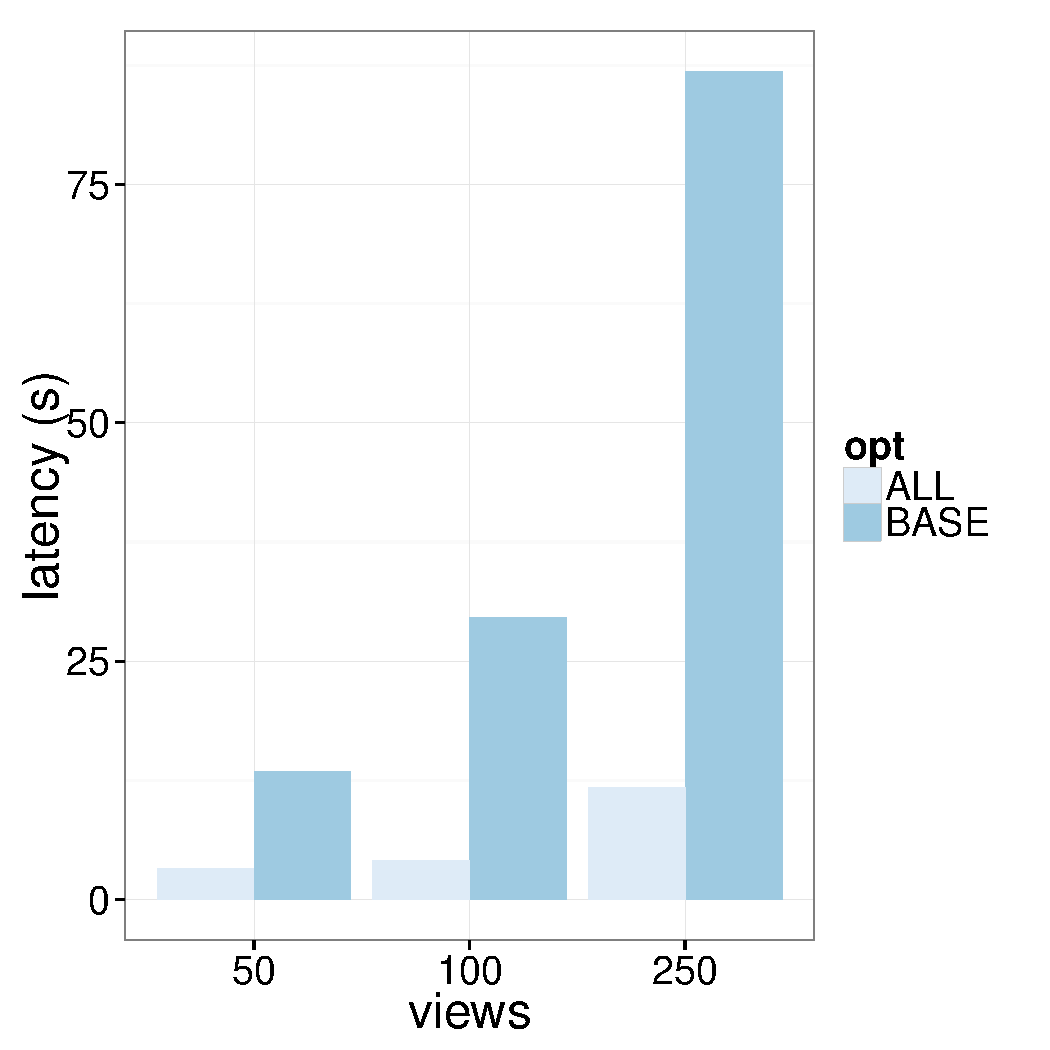
\includegraphics[width=4.6cm] {Images/col_all_none_by_views.pdf}}
		\caption{Column Store Latencies by Views}
		\label{fig:col_all_none_views}
	\end{subfigure}
	\caption{Effect of Combining Multiple Queries}
	\label{fig:all_opt}
\end{figure*}


% \begin{figure}[h]
% \centering
% \begin{subfigure}{0.49\linewidth}
% \centering
% {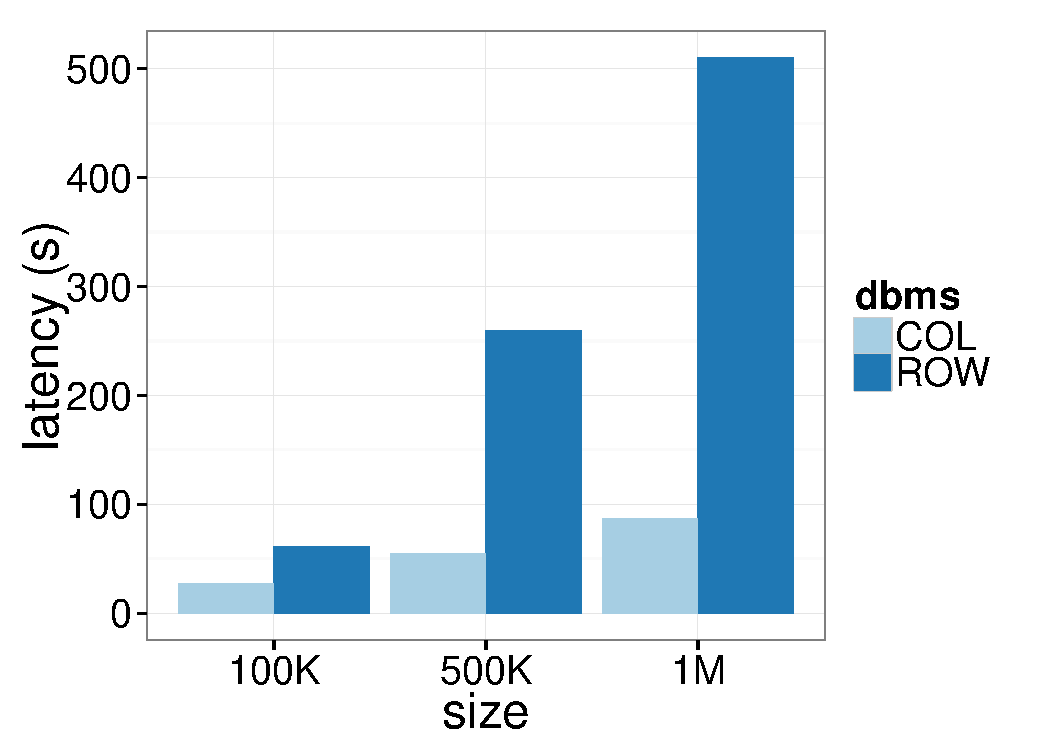
\includegraphics[width=4.2cm] {Images/baselines_by_size.pdf}}
% \caption{Latency vs. Table size}
% \label{fig:baseline_size}
% \end{subfigure}
% \begin{subfigure}{0.49\linewidth}
% \centering
% {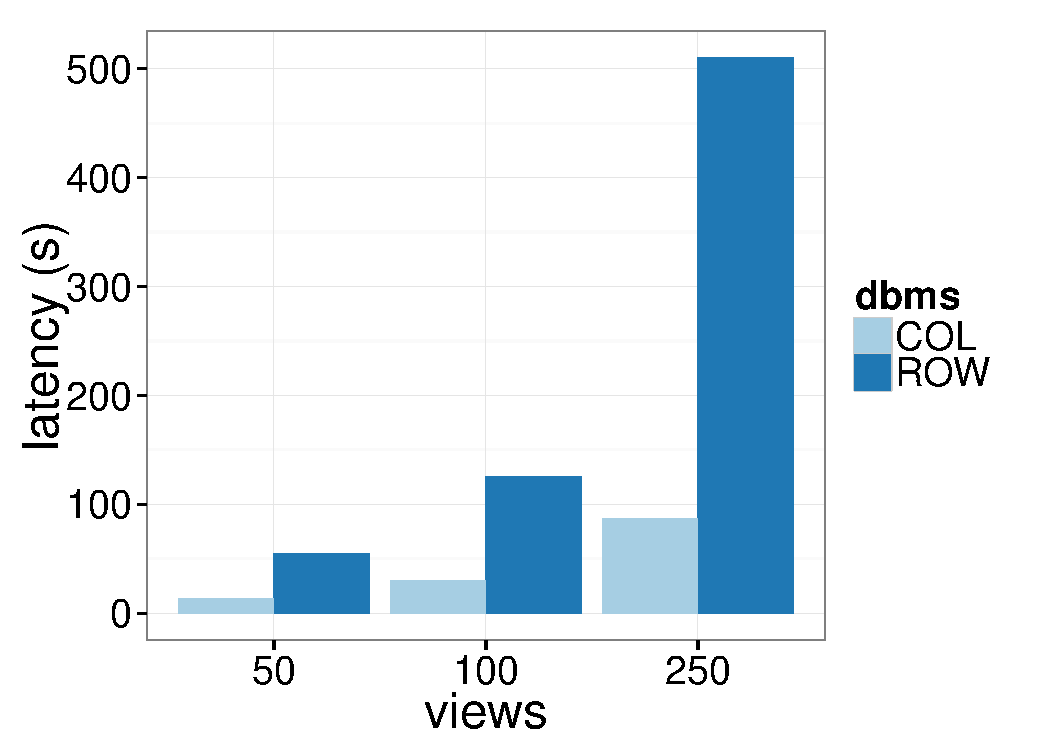
\includegraphics[width=4.2cm] {Images/baselines_by_views.pdf}}
% \caption{Latency vs. Num Views}
% \label{fig:baseline_views}
% \end{subfigure}
% \label{fig:baselines}
% \caption{Latency of Basic Framework}
% \end{figure}

\noindent {\it Combining Multiple Aggregates}: Next, we study the impact of
computing multiple aggregate functions within the same query.
The goal of this optimization is to evaluate multiple views at once by keeping
track of multiple aggregates for the same dimension (GROUP BY) attribute, as
described in Section~\ref{XXX}.
We ran these experiments on the SYN2 dataset since it has a large number (20) of
measure attributes.
In these experiments, we varied the number of aggregate attributes ($n_{agg}$)
in a query between 1 and 20 and measured \VizRecDB\ latency for each value of
$n_{agg}$.
Results of this experiment are shown in Figure \ref{fig:multi_agg}.
As we can see from this chart, latency drops consistently as we increase the
number of aggregations performed per query.
The latency reduction is however not quite linear in $n_{agg}$ because larger
$n_{agg}$ requires more state to the stored and, in the case of column stores, more
columns to be read.
This optimization shows significant speedups both in row and column stores: we
get a 4X speedup for row stores and a 3X speed up for column stores.\\

% \begin{figure}[h]
% \centering
% {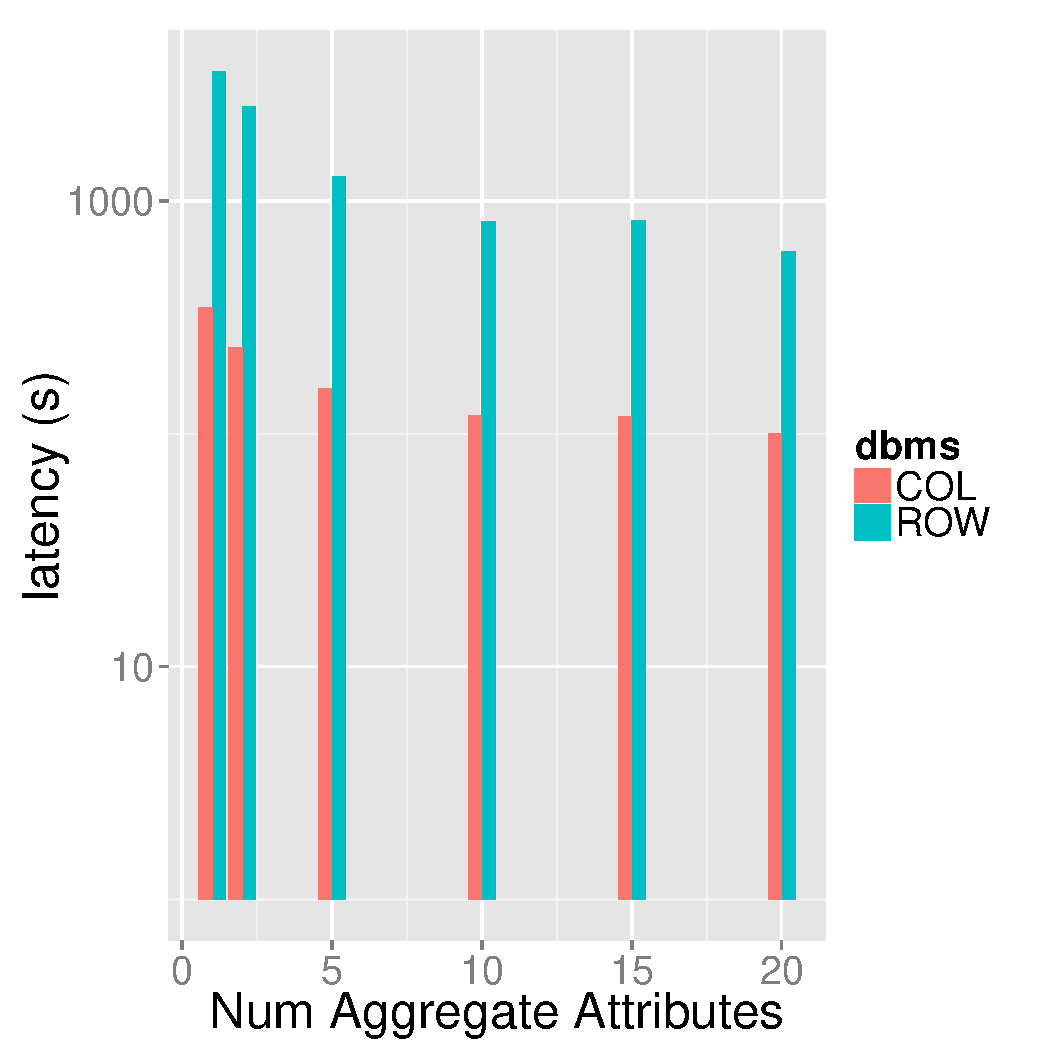
\includegraphics[width=6cm] {Images/multi_agg.pdf}}
% \caption{Latency vs. number of aggregates}
% \label{fig:multi_agg}
% \end{figure} 

\noindent {\it Combining Multiple Group Bys}: In this set of experiments, we
study the effect of combining multiple group by attributes into one query.
Section \ref{XXX} briefly discussed how the impact of this optimization was not
clear since it increases the total number of groups significantly and therefore
leads to higher costs of processing intermediate results.
To evaluate this optimization, we use the SYN3-10 and SYN3-100 datasets.
We chose these datasets over SYN1 and SYN2 since we wanted to exactly control
the number of distinct groups in every attribute and consequently the number of
distinct groups in every combination of attributes.
In SYN3-10 for example, all dimensions have 10 distinct values and each
dimension is independently generated. 
Therefore, the total number of distinct
groups produced by a query with $p$ group-by attributes is $max(10^p,
num\_rows)$.
SYN3-100 similarly has 100 distinct values per attribute and will produce
$max(10^p, num\_rows)$ groups for $p$ attributes.
Our goal in these experiments was to determine if (a) combining multiple
group-by attributes improved performance, and (b) whether it was the number of
group-by attributes or the number of distinct groups produced by a query that
predicted performance.

We ran \VizRecDB\ on SYN3-10 and SYN3-100, and varied the number of
group-by attributes in view queries ($n_{gb}$) between 1 and 20.
Figure \ref{fig:multi_gb_same} shows the results for this experiment.
We see that for the row-store, the best latency is obtained for number of
groups=$10^4$.
Beyond $10^5$, the performance degrades drastically.   \srm{same comment as
above -- we can't really have $10^{20}$ groups!} For the column-store, we see a
relatively small improvement in latency for $10^2$ groups, however, once again,
after $10^5$ groups, the performance becomes much worse.
The reason for this is as follows: as we combine group by attributes, the number
of distinct groups increases exponentially ($10^{n_{gb}}$).
As a result, the memory required for the grouping (hash-based or sort based)
also increases significantly.
Once this memory requirement exceeds the buffer space the system allocates for
intermediate results, the performance degrades significantly as the DBMS
switches to an external sort or hash algorithm.

% \begin{figure}[h]
% \centering
% \begin{subfigure}{0.49\linewidth}
% \centering
% {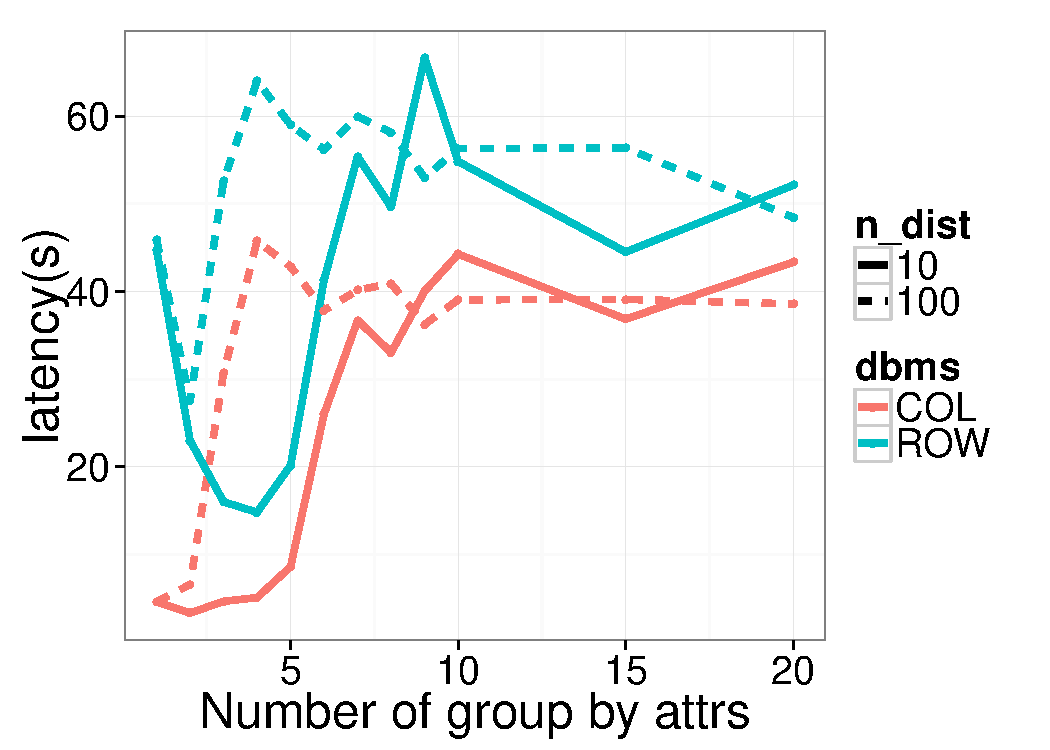
\includegraphics[width=4.2cm] {Images/multi_gb_same.pdf}}
% \caption{Latency vs. Num of Groups}
% \label{fig:multi_gb_same}
% \end{subfigure}
% \begin{subfigure}{0.49\linewidth}
% \centering
% {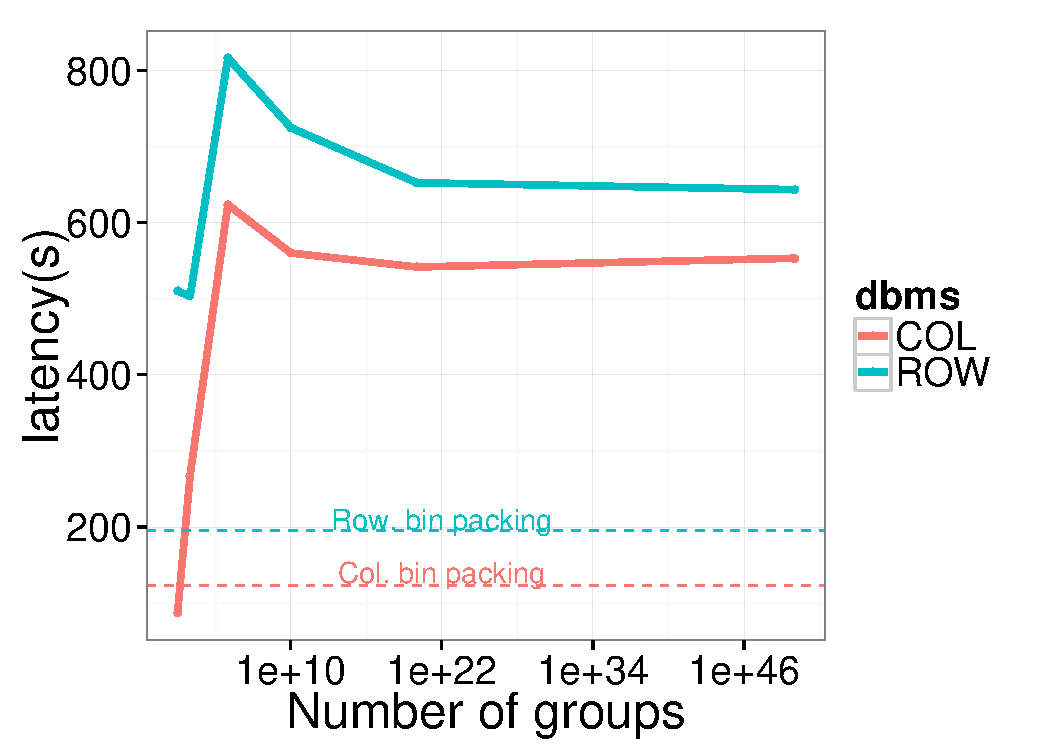
\includegraphics[width=4.2cm] {Images/multi_gb.pdf}}
% \caption{Latency vs. Num Dimensions}
% \label{fig:multi_gb_bp}
% \end{subfigure}
% \label{fig:multi_gb}
% \caption{Effect of combining multiple groups}
% \end{figure}

We can guard against the above performance degradation by ensuring that the
number of distinct groups never goes beyond a pre-configured upper limit.
From Figure \ref{fig:multi_gb_same}, we see that this limit is approximately
$10^5$ for both the row and column store.
With knowledge of this upper limit on the number of distinct groups, we can now
apply our grouping technique based on bin packing (Section \ref{}) to optimally
group the dimension attributes.
Bin-packing ensures that the number of distinct groups produced by any query is
less than $10^5$.
Figure \ref{fig:multi_gb_bp} shows the results of two grouping strategies: (a)
the bin packing-based strategy, and (b) grouping based on number of attributes.
In the latter strategy, we randomly group attributes into groups of size
$n_{gb}$. 
Since the latency for this strategy will depend on the particular grouping of
attributes, we repeated this experiment 20 times and report the average latency.
Figure \ref{fig:multi_gb_bp} shows the result for SYN1 where $n_{gb}$ was varied
between 1 and 20.
The dotted lines indicate the latency of the bin packing-based grouping strategy
whereas the solid lines indicate the latency of grouping based on attribute
number.
As we can see from the chart, bin-packing is always superior to grouping
based on attribute number.
We see that for the row-store, bin-packing reduces latency by a factor of 2X. 
What about column store???\\

\noindent {\it Parallel Query Execution}: 
Executing view queries in parallel can provide significant performance gains;
however, a high degree of parallelism can lead to a performance drop off for
several reasons. Potential reasons include disk contention, RAM usage, lock
contention, context switches and cache line contention \cite{Postgres_wiki}. 
Figure \ref{fig:parallelism} illustrates this issue: we varied the number of
queries running in parallel on the DBMS and measured the latency of
\VizRecDB.
As expected, low levels of parallelism produce sizable performance gains but
high levels of parallelism lead to degraded performance.
For our system, the optimal number of queries to run in parallel is
approximately $16$ (equal to the number of cores). 
In general, choosing a degree of parallelism equal to the number of cores
for these kinds of simple aggregation queries when data largely fits in memory
is a reasonable rule of thumb.  \\
%For other systems, we recommend users that they set the number of parallel
%queries to the maximum number of parallel queries that can be run in
%their DBMS without performance degradation.
%If this number is not easily available, a simple experiment as shown in Figure
%\ref{fig:parallelism} can help approximate the right amount of parallelism. \\

% \noindent {\it Combining Target and Comparison Views}:
% The last optimization we evaluate is that of combining the target and comparison
% views and running a single SQL query per view as opposed to two.
% We expected this optimization to roughly halve the latency since each query
% takes one table scan instead of two.\\

\noindent {\it All optimizations}:
Now that we have explored all our optimizations in detail, we pick the optimal
parameters discovered above and combine our optimizations to get the maximum
performance gain.
For the row store, we applied all the above optimizations with $n_{agg}$ set to
the number of measure attributes, maximum number of group-bys set to $10^5$ and
number of parallel queries set to $16$.
For the column store, we set $n_{agg}$ and number of parallel queries similarly
but did not apply the group-by optimization. 
Figures \ref{fig:all_opt}a-d show the latency of \VizRecDB\ on SYN1 when all
optimizations have been applied.
From Figures \ref{fig:row_all_none_size} and \ref{fig:row_all_none_views}, we
see that for the row store, our optimizations lead to a speedup of up to 20X
across a range of sizes and views.
Similarly, in Figures \ref{fig:col_all_none_size}
and \ref{fig:col_all_none_views}, we see that our optimizations lead to a 8x
speedup.
We also notice that our optimizations are most effective for datasets with large
sizes and many views.
This experiment shows that the application of well designed optimizations
can reduce \VizRecDB\ latency by 8-20X depending on the DBMS and enable a
\VizRecDB-style workload to run in interactive time scales.

In the next section, we evaluate our custom execution engine and
its pruning heuristics to evaluate the performance and accuracy implications of
pruning.

\subsection{Custom Execution Engine}
\label{sec:custom_execution_engine}

As discussed in Section \ref{}, we built a custom execution engine for
\VizRecDB\ that can share table scans across all views and use intermediate
results to prune low-utility views.  
Through the next set of experiments, we evaluate the various pruning heuristics
we developed for the custom execution engine.
Our goal is to determine the effectiveness of our strategies pruning
low-utility views and their impact on \VizRecDB\ latency.
In each of our experiments, we evaluate heuristics along three metrics:
{\it latency, accuracy} and {\it utility distance}.
As in the previous section, latency is defined as the total time taken by
\VizRecDB\ to return the top-$k$ views and is averaged over 3 runs.
Accuracy is the number of true top-$k$ views that are present in the
top-$k$ views returned by our algorithm.
Finally, utility distance is the difference between the average utility of
the true top-$k$ views and the average utility of the top-$k$ views generated by
our algorithm.
Since the accuracy and utility distance of our techniques are influenced by the
order in which data is read in, we repeat each experiment 20
times and randomize the data between runs. We report average
metrics over 20 runs.

Notice that our goal is not to directly compare the latency of our custom
execution engine to the latency of the heavily optimized DBMS-backed execution
engine.
Naturally, the DBMS-backed engine benefits from the significant optimizations
present in modern day DBMSs such as vecorization, compression, ability to
exploit multiple cores etc. that make it highly performant. 
Insetad, our goal is to evaluate the performance improvements that can be
obtained by pruning and sharing table scans.

% that have gone into We believe that comparing such
% systems offers little value:
% on one hand, our custom implementation lacks features such as logging or
% concurrency control that can slow down more complete systems; on the other hand,
% it also lacks optimizations for exploiting multiple cores, compression,
% vectorization, and other optimizations that scan-optimized column-stores employ.
% Rather, our goal is to highlight the relative performance benefits that can be
% obtained by performing pruning and shared scans.

Since it is hard to capture the complexities of real data distributions in synthetic data, we
evaluate all our pruning strategies on real-world data. 
Specifically, we make use of the BANK AND DIAB datasets listed in Table
\ref{tab:datasets}.
\begin{compactitem}
\item {\it Diabetes data}\cite{}: This dataset contains records of hospital
visits by patients with diabetes. Records include patient demographics,
diagnoses, number of days at the hospital, procedures performed etc. 
This dataset contains 100K records and ~80 views.
\item {\it Bank dataset}\cite{}: This dataset contains records of customers who
applied for a loan. It includes demographic information about the
customers, information about the bank's previous contact with the customer, and
the ultimate decision on the loan.
This dataset contains 40K records and ~70 views.
\end{compactitem}
We chose these datasets since they contained a mix of numerical and categorical
attributes and were comparable to other analytical datasets in size.

For each of the above datasets, we evaluate 4 pruning strategies:
(a) No Pruning (NO\_PRU): we make a single pass of the data and keep running
estimates for the utility of every possible view. Once we have seen all the
data, we return the top-$k$ views with highest utility; (b) Hoeffding Intervals
(HOEFF):
we use pruning based on Hoeffding intervals (Section \ref{}); (c) 95\%
Confidence Intervals (95\_CI): we use pruning based on 95\% confidence intervals
(Section \ref{}); and (d) Multi-armed Bandit (MAB): we perform pruning based on
the multi-armed bandit formulation (Section \ref{}).
For each of our datasets, we varied $k$, the number of views to select, between
1 and 25 (a realistic upper limit on the number of views displayed to the user)
and measured the latency, accuracy and utility distance for each of our
heuristics.

We begin with an evaluation of our techniques with respect to their accuracy
and utility distance.\\

\begin{figure}[h]
	\centering
	\begin{subfigure}{1\linewidth}
		\centering
		{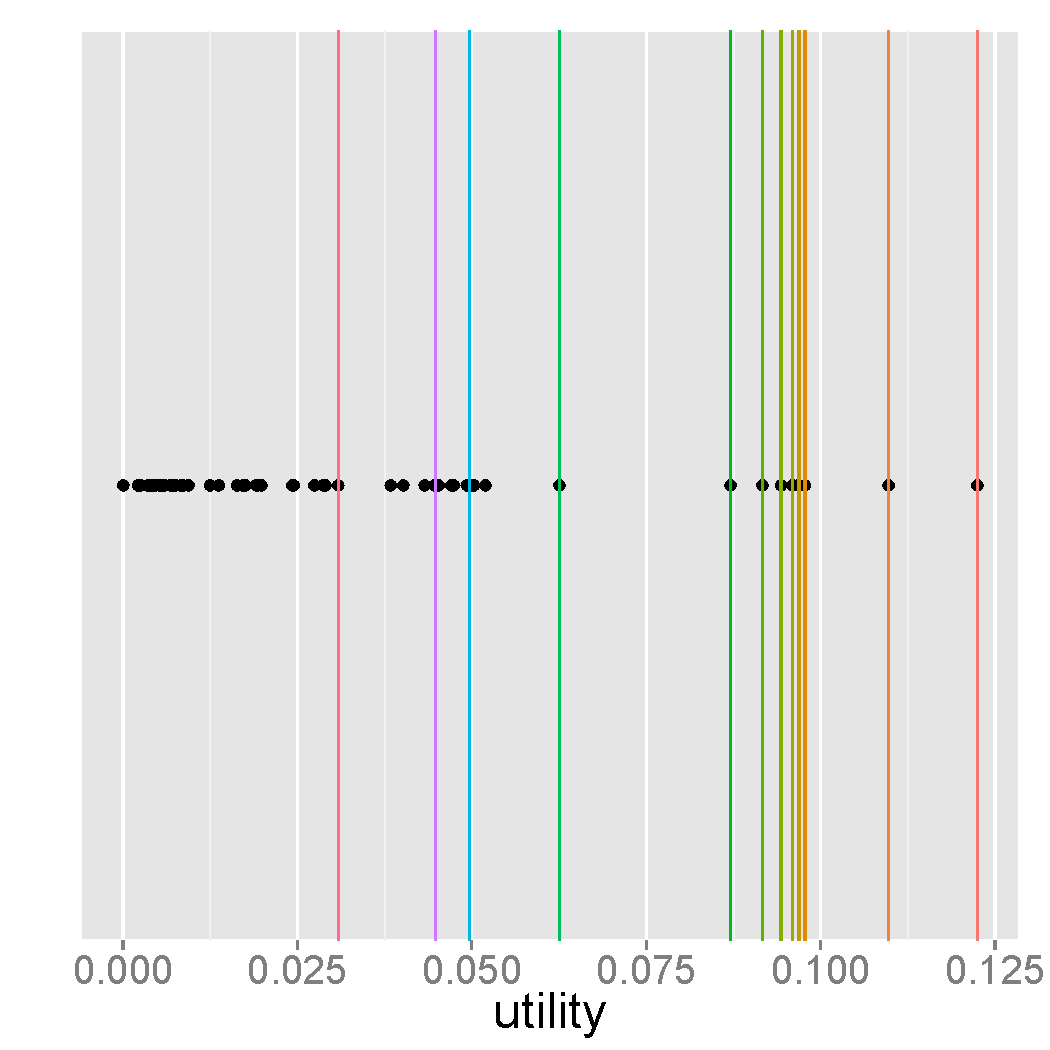
\includegraphics[trim = 0mm 60mm 0mm 60mm, clip, width=8cm]
		{Images/bank_utility_distribution.pdf}}
		\caption{Bank dataset: utility distribution}
		\label{fig:bank_utility_distribution}
	\end{subfigure}
	
	\begin{subfigure}{1\linewidth}
		\centering
		{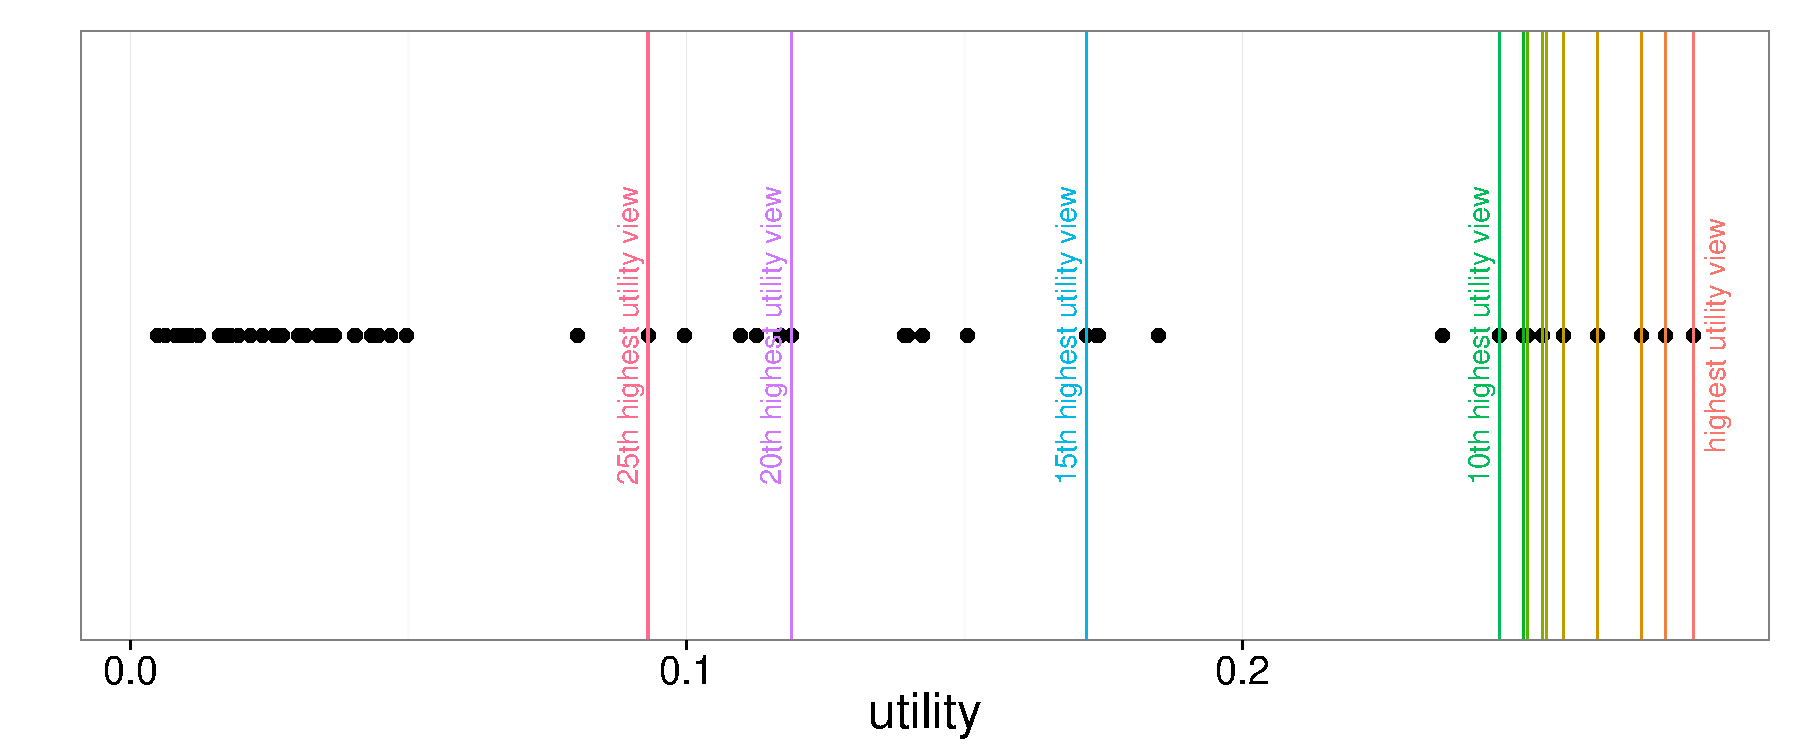
\includegraphics[trim = 0mm 60mm 0mm 60mm, clip, width=8cm]
		{Images/diabetes_utility_distribution.pdf}}
		\caption{Diabetes dataset: utility distribution}
		\label{fig:diabetes_utility_distribution}
	\end{subfigure}
\label{fig:utility_distribution}
\caption{Distribution of Utilities}
\end{figure}


\noindent {\it Accuracy and Utility Distance}:
Let us examine the banking dataset first.
The distribution of utilities for all views of the banking dataset is
shown in Figure \ref{fig:bank_utility_distribution}. 
In this chart, vertical lines denote the cutoffs for utilities for top-$k$ views
where $k$=\{1\ldots10,15,20,25\}.
The highest utility for this dataset corresponds to the {\it right-most} line
in this chart while the 25-th highest utility corresponds to the {\it left-most}
line.
From the chart we see that the
highest and second highest utility are spread well apart from the rest of the
utilities.
We also observe that the top 3rd--9th utilities are rather similar. 
The 10th highest utility is again separated from neighboring utilities by a
large value and then the remaining utilities are again close together.
This distribution of utilities directly impacts the performance of our pruning
techniques since utilities that are close together have very similar running
estimates of utility and hence are difficult to tease apart and prune.
Utilities that are spread apart, in contrast, have estimates that are also
spread apart and we can prune views easily.

We see that the impact of this utility distribution in the accuracy chart in
Figure \ref{fig:bank_accuracy}.
We find that the average accuracy of all three heuristics is reasonable for
$k$=1 and 2 (recall that these are spread apart from the other utilities).
However, between $k$=3\ldots9, the accuracy suffers (consequence of similar
utility values).
After $k$=10, the performance of all our heuristics improves once again.

Now, let us examine how ``bad'' our errors are in finding the top-$k$ views.
We do so by looking at the utility distance (i.e. the distance between
the average utility of the true top-$k$ views and the average utility of the
top-$k$ views picked by our strategies).
Utility distance gives us an easy way to measure how far we are from the true
top-$k$ views.
Figure \ref{fig:bank_utility_dist} shows the utility distance for
all of our heuristics for the bank dataset.
The NO\_PRU technique necessarily has 0 utility distance since
it performs no pruning.
We add an extra ``strategy'' here which is the random strategy (RANDOM).
It essentially means that we chose any $k$ views at random and computed their
utility distance.
This strategy serves as a lowerbound on the quality of our results.
Notice that all of our heuristics are significantly better than the RANDOM
strategy for all $k$s.
All of our heuristics produce views with 0 or almost 0 utility distance. 
Thus, there is effectively no difference in the utilities of the top $k$ views
we select vs. the true top-$k$ views.
So even when a top-$k$ strategy picks a few incorrect views, the selected views
have utility very close to the real top-$k$ views, i.e., are views are
approximate but of high quality.
% This implies that even if our top-$k$ views are
% approximate, they are of high quality.
% Another way to analyze mistakes in the top-$k$ views is by examining if the an
% incorrectly returned view for the top-$k$ views also appears in the top-$2k$,
% top-$3k$ or top-$4k$.
% Figure \ref{} shows the results for the banking dataset.
% We see that XXX,

\begin{figure*}[t]
	\centering
	\begin{subfigure}{0.33\linewidth}
		\centering
		{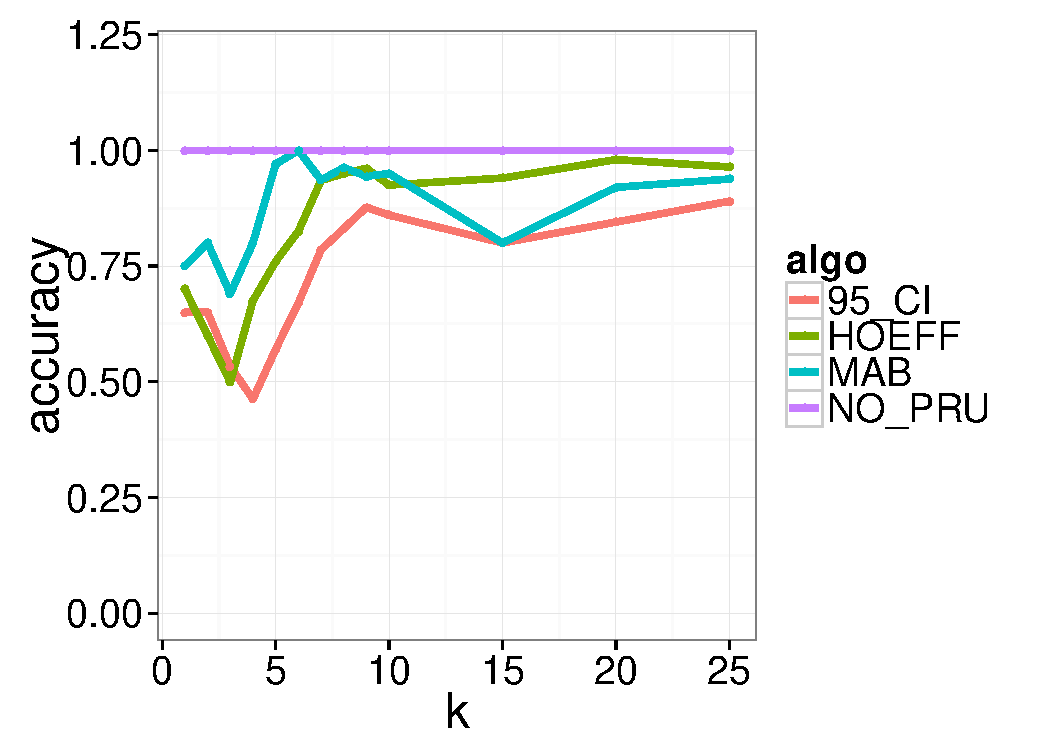
\includegraphics[width=6cm] {Images/in_memory_bank_accuracy.pdf}}
		\caption{Accuracy}
		\label{fig:bank_accuracy}
	\end{subfigure}
	\begin{subfigure}{0.33\linewidth}
		\centering
		{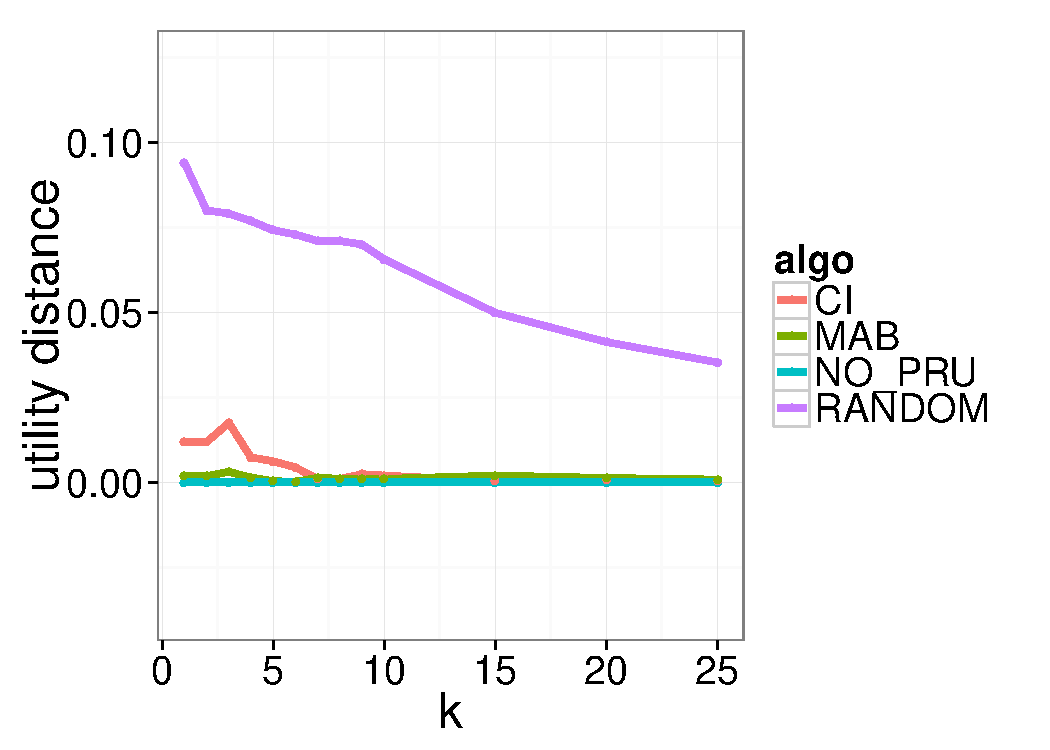
\includegraphics[width=6cm] {Images/in_memory_bank_utility_dist.pdf}}
		\caption{Utility Distance}
		\label{fig:bank_utility_dist}
	\end{subfigure}
	\begin{subfigure}{0.33\linewidth}
		\centering
		{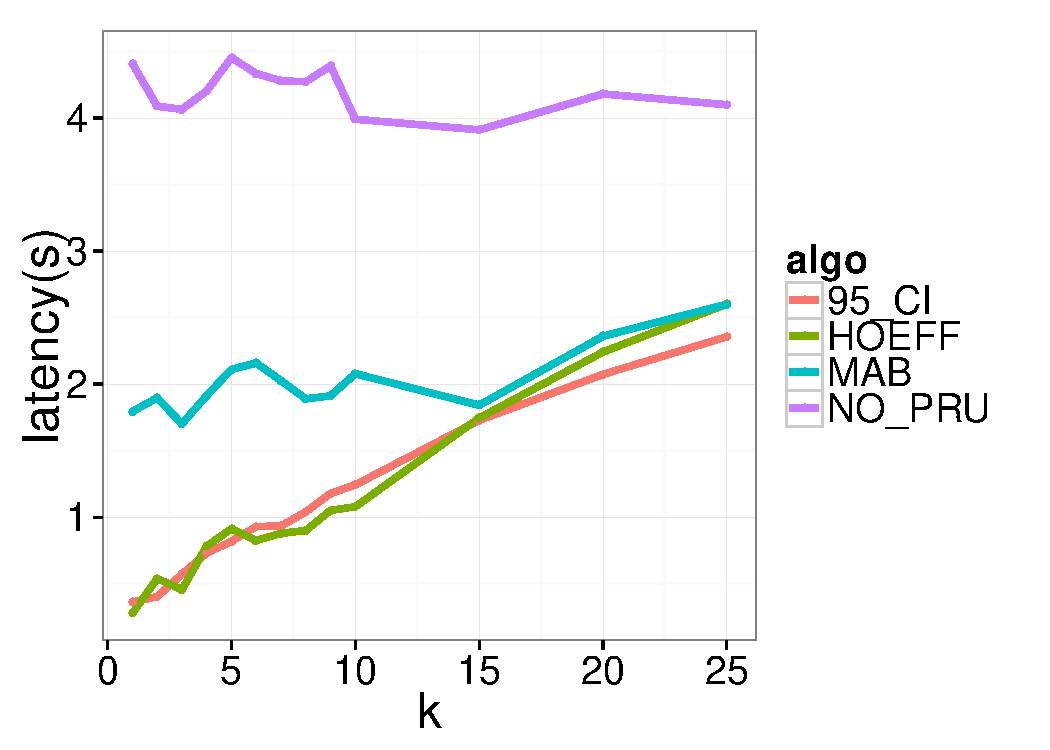
\includegraphics[width=6cm] {Images/in_memory_bank_latency.pdf}}
		\caption{Latency}
		\label{fig:bank_latency}
	\end{subfigure}
	\caption{Performance of heuristics for Bank dataset}
	\label{fig:bank_perf}
\end{figure*}

\begin{figure*}[t]
	\centering
	\begin{subfigure}{0.33\linewidth}
		\centering
		{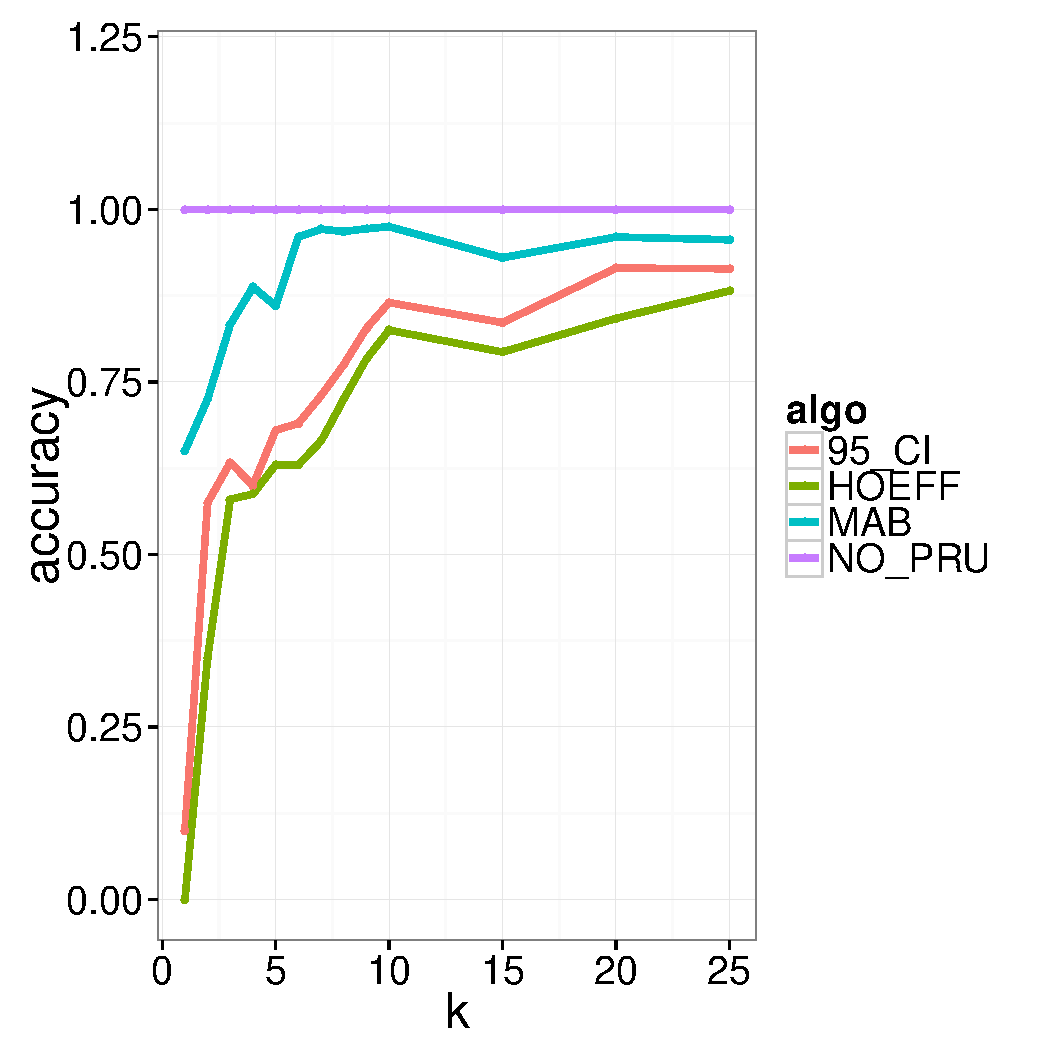
\includegraphics[width=6cm] {Images/in_memory_dia_accuracy.pdf}}
		\caption{Accuracy}
		\label{fig:dia_accuracy}
	\end{subfigure}
	\begin{subfigure}{0.33\linewidth}
		\centering
		{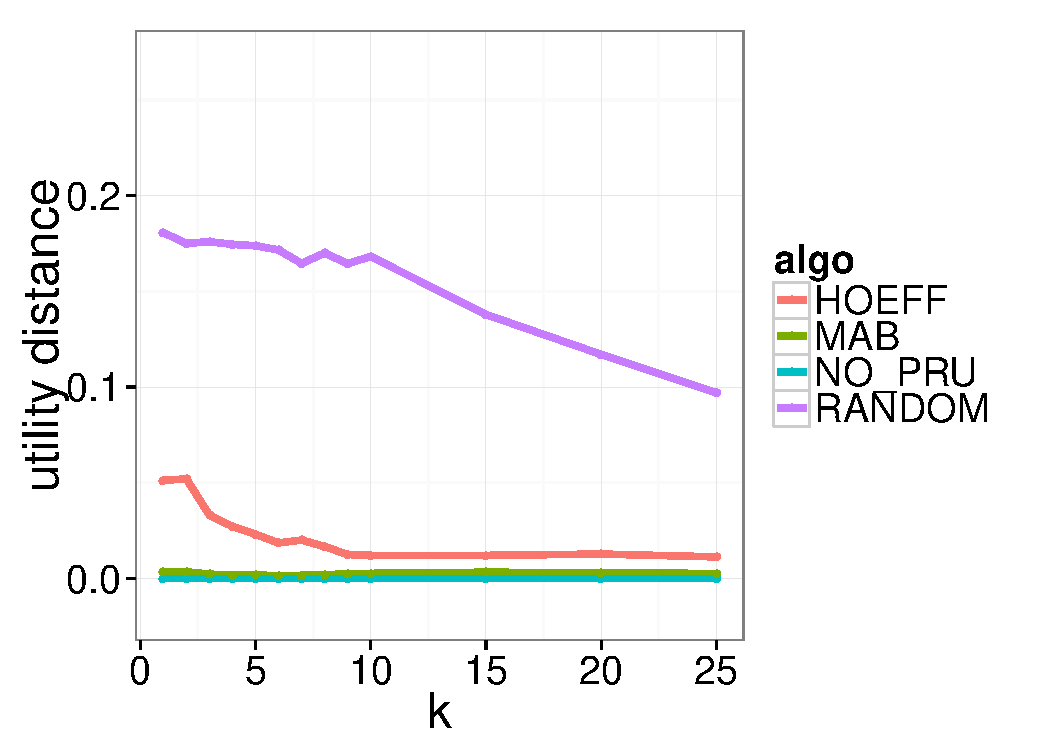
\includegraphics[width=6cm] {Images/in_memory_dia_utility_dist.pdf}}
		\caption{Utility Distance}
		\label{fig:dia_utility_dist}
	\end{subfigure}
	\begin{subfigure}{0.33\linewidth}
		\centering
		{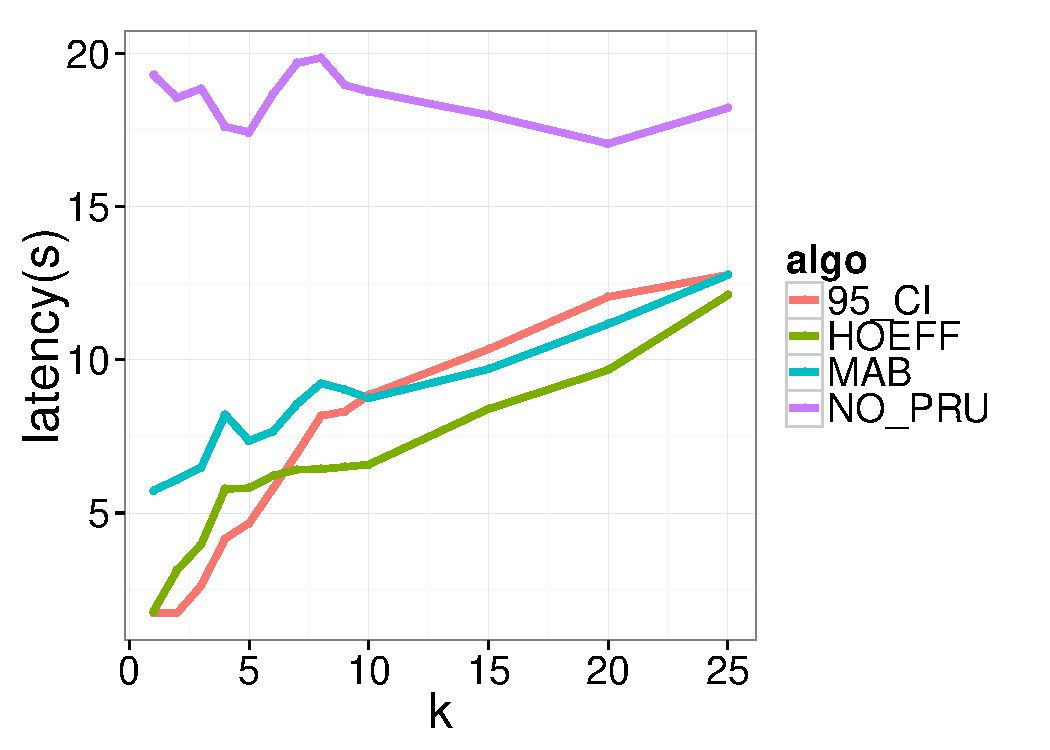
\includegraphics[width=6cm] {Images/in_memory_dia_latency.pdf}}
		\caption{Latency}
		\label{fig:diabetes_latency}
	\end{subfigure}
	\caption{Performance of heuristics for Diabetes dataset}
	\label{fig:diabetes_perf}
\end{figure*}

% \begin{figure}[h]
% \centering
% \begin{subfigure}{0.49\linewidth}
% \centering
% {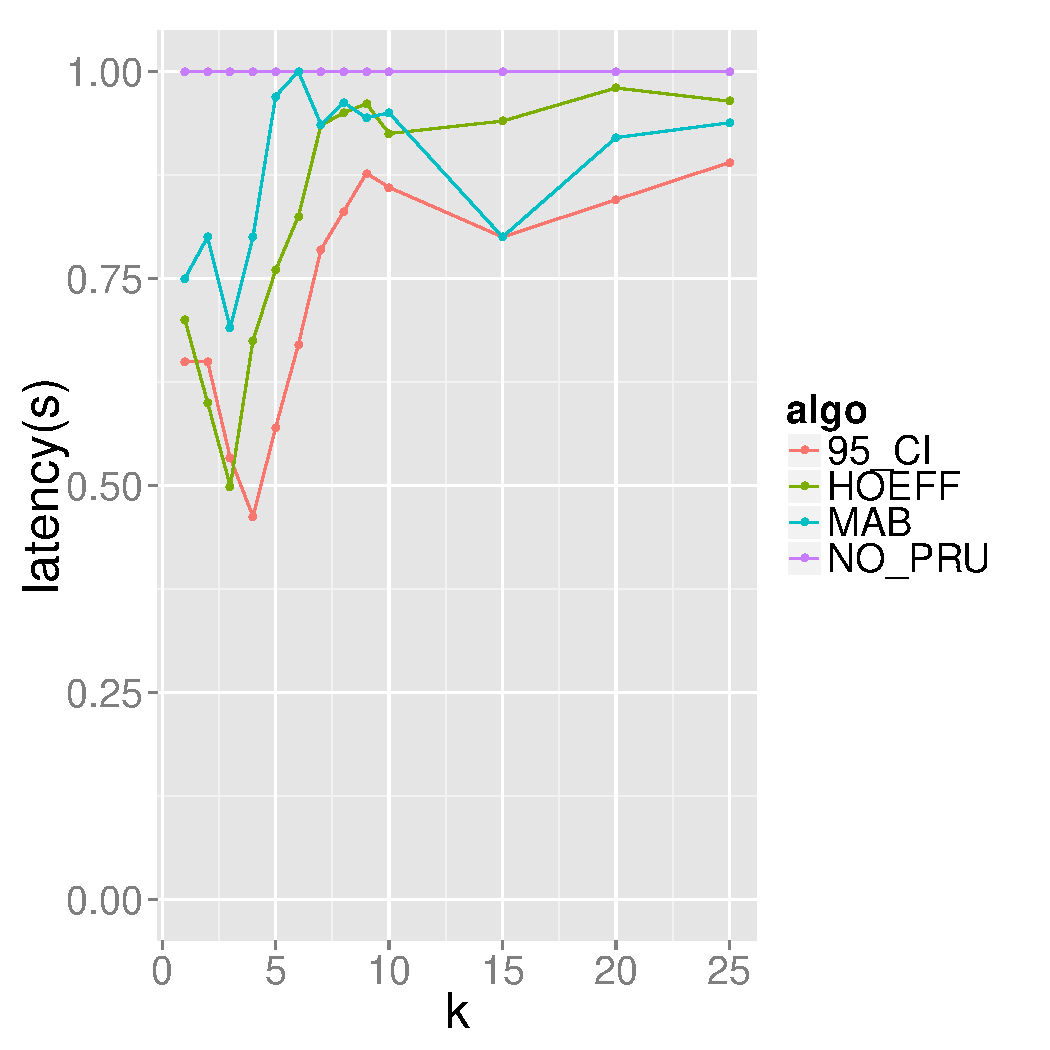
\includegraphics[width=4.2cm] {Images/bank_in_memory_accuracy.pdf}}
% \caption{Accuracy of heuristic for bank dataset}
% \label{fig:bank_accuracy}
% \end{subfigure}
% \begin{subfigure}{0.49\linewidth}
% \centering
% {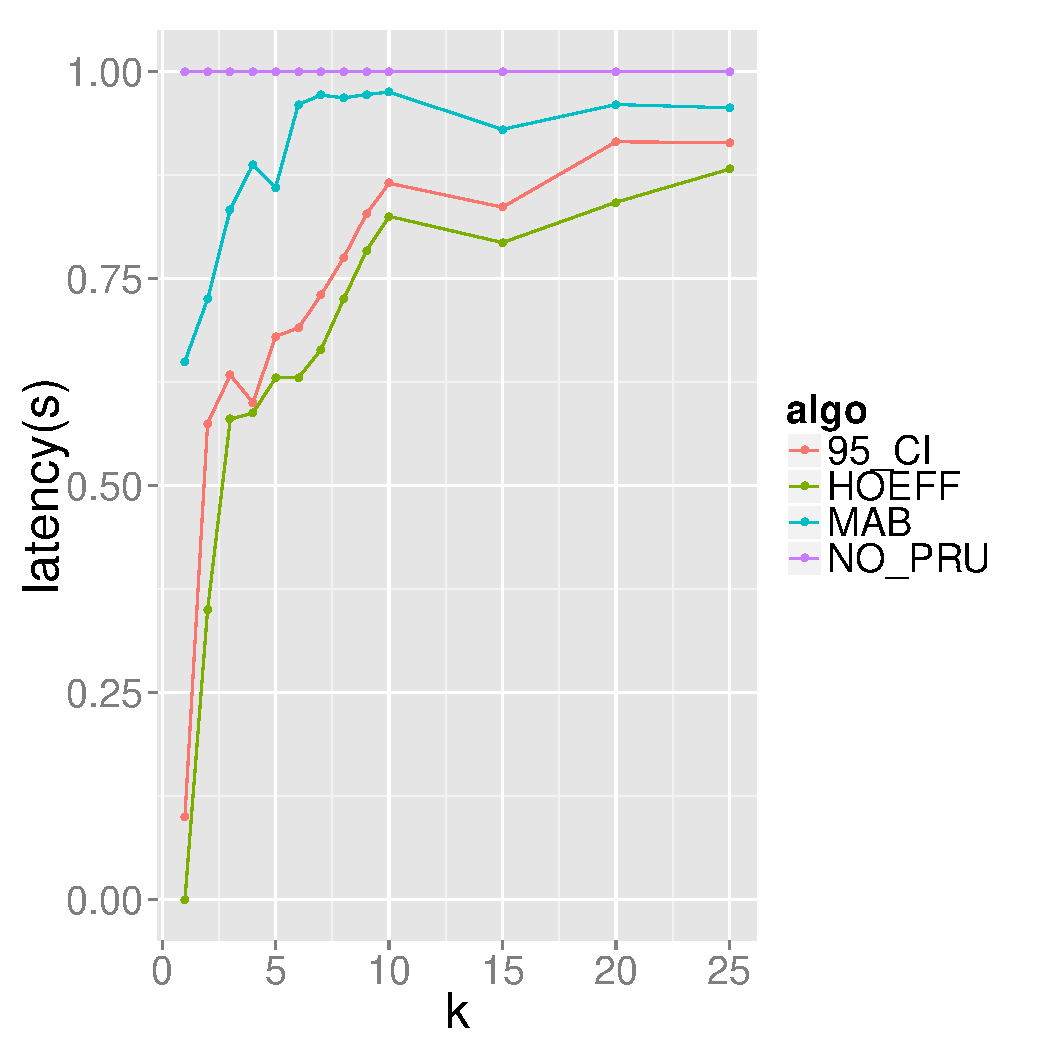
\includegraphics[width=4.2cm] {Images/dia_in_memory_accuracy.pdf}}
% \caption{Accuracy of heuristics for diabetes dataset}
% \label{fig:dia_accuracy}
% \end{subfigure}
% \label{fig:accuracy}
% \caption{Accuracy of Heuristics}
% \end{figure}


% \begin{figure}[h]
% \centering
% \begin{subfigure}{0.49\linewidth}
% \centering
% {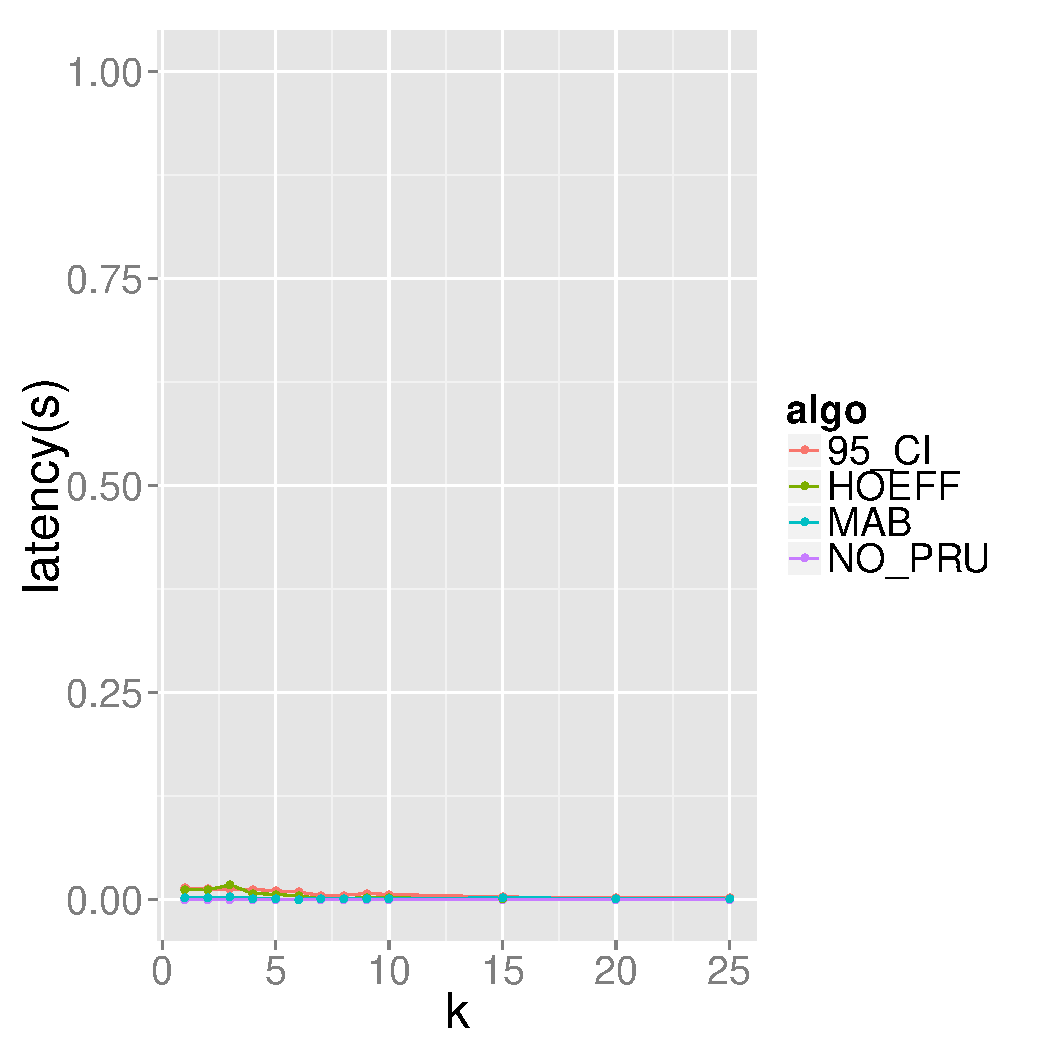
\includegraphics[width=4.2cm] {Images/bank_in_memory_utility_dist.pdf}}
% \caption{Utility Distance of heuristic for bank dataset}
% \label{fig:bank_utility_dist}
% \end{subfigure}
% \begin{subfigure}{0.49\linewidth}
% \centering
% {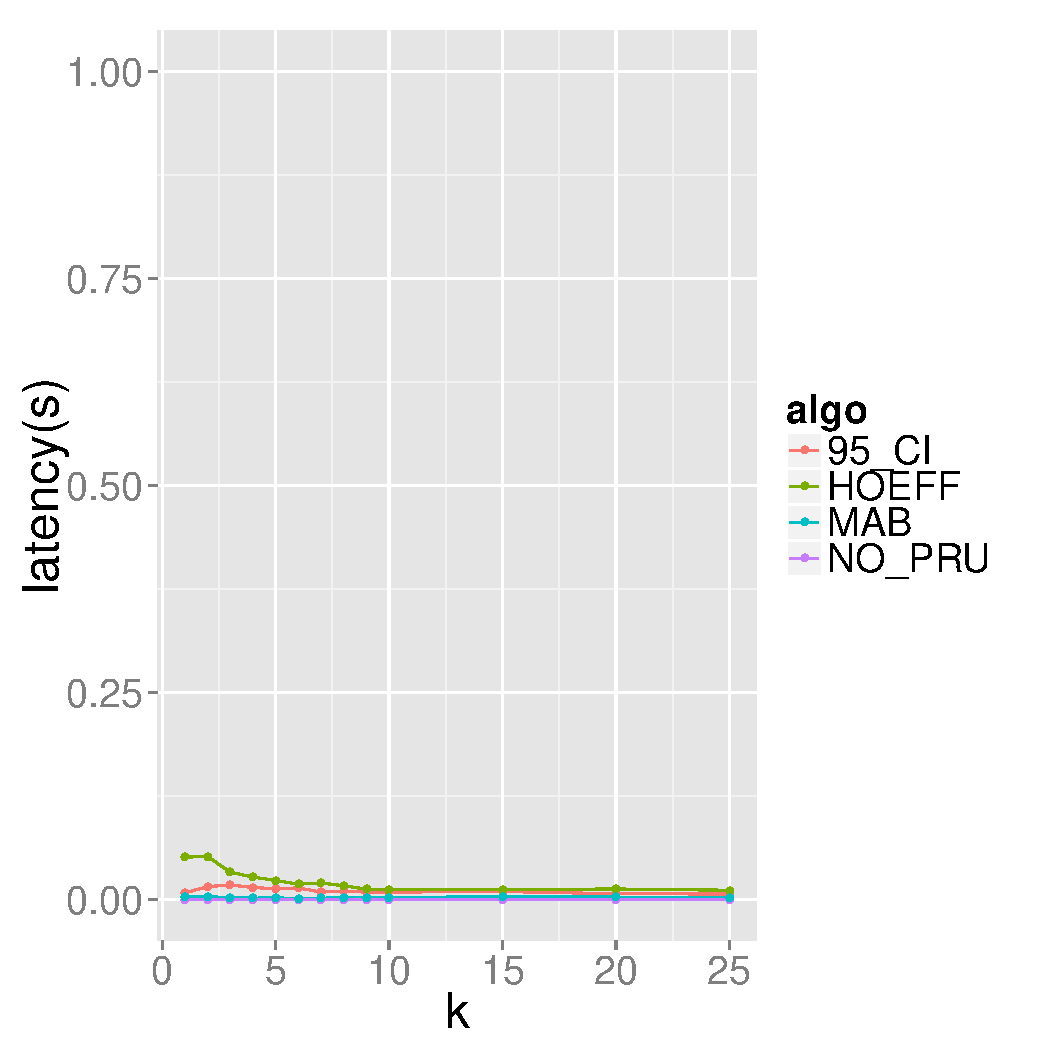
\includegraphics[width=4.2cm] {Images/dia_in_memory_utility_dist.pdf}}
% \caption{Utility Distance of heuristics for diabetes dataset}
% \label{fig:dia_utility_dist}
% \end{subfigure}
% \label{fig:accuracy}
% \caption{Utility Distance for Heuristics}
% \end{figure}

% \begin{figure}[h]
% \centering
% {\includegraphics[trim = 0mm 50mm 0mm 50mm, clip, width=6cm]
% {Images/bank_utility_distribution.pdf}}
% \caption{Bank dataset: utility distribution}
% \label{fig:bank_utility_distribution}
% \end{figure}
% \begin{figure}[h]
% \centering
% {\includegraphics[trim = 0mm 50mm 0mm 50mm, clip, width=6cm]
% {Images/diabetes_utility_distribution.pdf}}
% \caption{Diabetes dataset: utility distribution}
% \label{fig:diabetes_utility_distribution}
% \end{figure}
 
Next, let us examine the results for the diabetes dataset.
The distribution of true utilities for all views in this dataset are shown in
Figure \ref{fig:diabetes_utility_distribution}.
Compared to the bank dataset, we see that utilities are very closely
clustered for top 1\ldots10 views.
On the other hand, the utilities around $k$=15, 20 and 25 are relatively widely
spaced.
As a result, we expect lower pruning accuracy for $k<10$ but high accuracy for
large $k$'s.
We see this behavior in Figure \ref{fig:dia_accuracy} where the accuracy of
pruning is quite low for small $k$s, increases until $k$=10 and then levels off.
A similar trend is seen in Figure \ref{fig:dia_utility_dist} showing that
utility distance is small for $k<10$ and then reduces to almost 0 for larger
$k$s.

We also observe an important property of our heuristics: the accuracy of all
three of our heuristics, MAB, 95\_CI and HOEFF, is comparable; MAB appears to
perform better for small number of $k$s but all three produce similar results
for $k>10$. (NO\_PRU is guaranteed to have perfect accuracy).
This suggests that since all heuristics perform similarly on accuracy, we can
choose the heuristic with the minimum latency.\\

% 95\_CI does the best among all our heuristics for the whole range of $k$ values.
% MAB and HOEFF produce similar accuracy values with MAB being slightly better
% than HOEFF.
% There are a few reasons why 95\_CI performs better: the MAB heuristic is tied to
% either accepting or discarding a view at the end of each phase; therefore, even
% if MAB is not very confidence in the action of accepting or discarding, it must
% reduce one view in each phase. HOEFF on the other hand is less accurate because
% XXX.
% All our heuristics however seem to have low accuracy for $k<10$. 

\noindent {\it Latency}:
Next, let us look at how long it takes for each of our pruning strategies to
work.
Figures \ref{fig:bank_latency} and \ref{fig:diabetes_latency} show the latency
of our heuristics for the banking and diabetes dataset.
The two charts look quite similar.
First off, we observe that {\it the use of any of our heuristics reduces the
latency by about 50\%}.
For NO\_PRU and 95\_CI, for small $k$'s, we obtain almost a 90\% reduction in
latency. However, as we saw earlier, some of this reduction in latency is
obtained at the cost lower accuracy.
We observe that the latency of HOEFF and 95\_CI increases almost linearly
with $k$.
Roughly speaking, this trend arises because as $k$
increases, we throw out fewer views and therfore perform more
computation per record.
This exact trend is not seen in MAB because MAB's pruning of views is agnostic
to the number of views that must be selected.

In general, we see that it is possible to reduce latency by 50\% just by using
any of our heuristics.
In fact, if we are willing to tradeoff some accuracy, we can cut latency by
90\%.
The next set of experiments vary the parameters for each heuristic to study
the accuracy vs. latency tradeoff.\\

% \begin{figure}[h]
% \centering
% \begin{subfigure}{0.49\linewidth}
% \centering
% {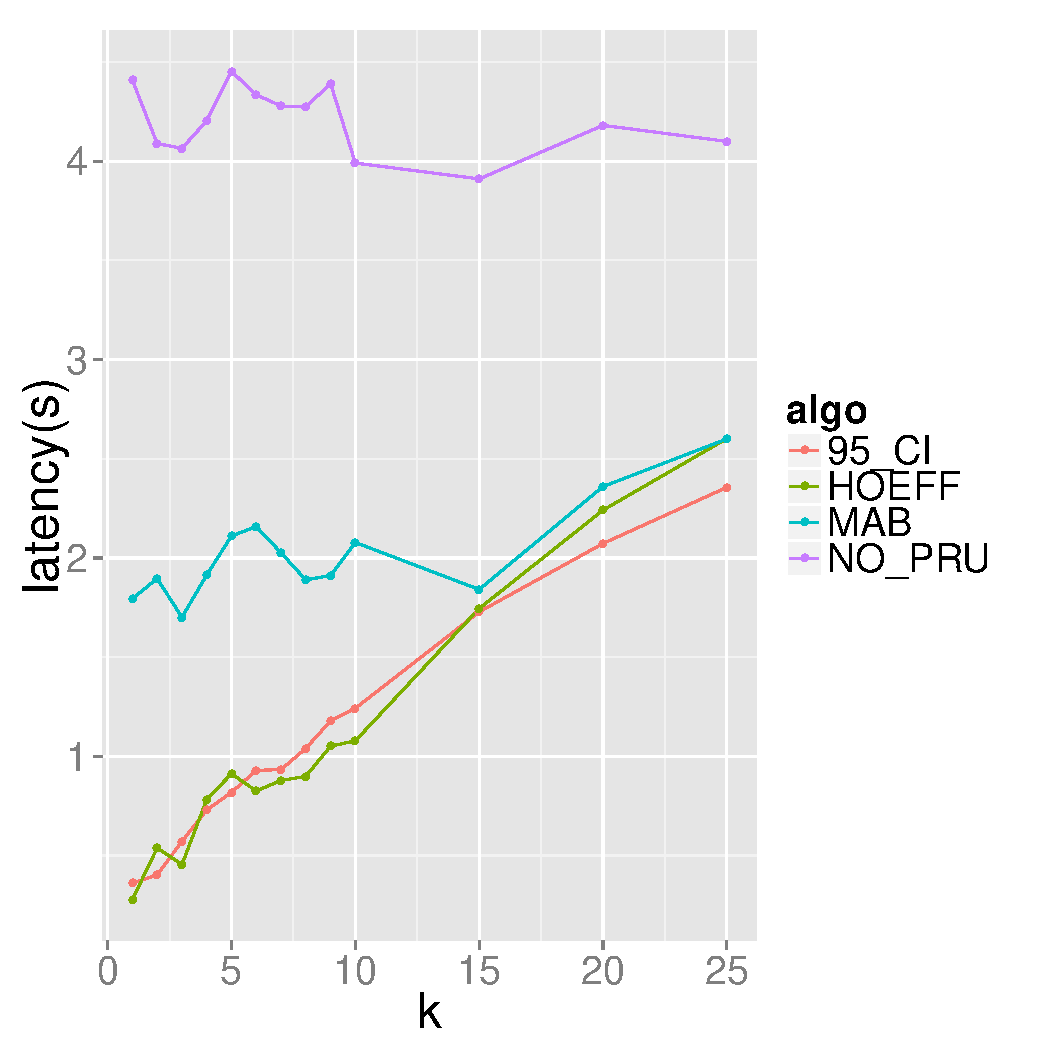
\includegraphics[width=4.2cm] {Images/bank_in_memory_latency.pdf}}
% \caption{Bank dataset: latency}
% \label{fig:bank_latency}
% \end{subfigure}
% \begin{subfigure}{0.49\linewidth}
% \centering
% {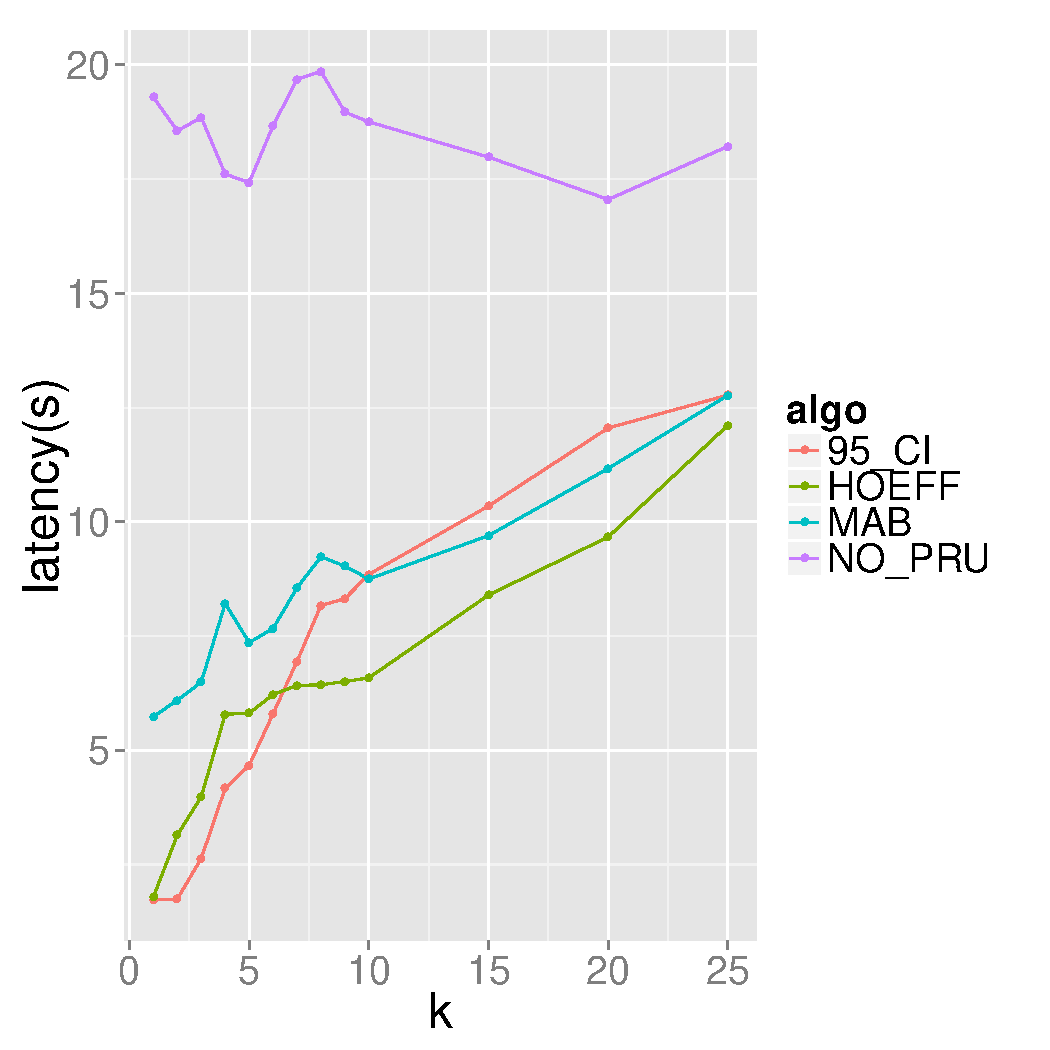
\includegraphics[width=4.2cm] {Images/dia_in_memory_latency.pdf}}
% \caption{Diabetes dataset: latency}
% \label{fig:diabetes_latency}
% \end{subfigure}
% \label{fig:accuracy}
% \caption{Latency for Heuristics}
% \end{figure}

\noindent {\it Accuracy vs. Latency}:
Our MAB and 95\_CI heuristics both have ``knobs'' we can use to study the
tradeoff between accuracy and latency.
In MAB, for example, we can tune the number of phases involved in
processing the entire file. 
Since MAB reduces the number of views by 1 after each phase, the number of
phases is proportional to the pruning power of our algorithm.
A large number of phases means that MAB will prune more views and will prune
them more often.
While this will lead to lower latency, it will also lead to lower accuracy.
Figure \ref{fig:latency_vs_accuracy_mab} shows how latency and accuracy both
reduce as we increase the number of phases in MAB ($k$=15).
Each point on the chart corresponds to a different setting for the number of
phases uses in that implementation of the MAB heuristic.
For 95\_CI, we can vary the $z$-score used
to determine the size of our confidence intervals.
That is, we can decide to take a 50\% confidence interval or a 80\% interval or
a 95\% interval.
If we take a smaller confidence interval, we will have higher pruning and
therefore lower latency.
However, a smaller confidence interval also leads to lower latency since we
prune views with lower confidence.
Figure \ref{fig:latency_vs_accuracy_ci} shows that as the $z$-score of the
confidence interval increases, the accuracy of our heuristics increases, but so
does its latency ($k$=15).
Every point corresponds to a different size of the confidence intervals.

\begin{figure}[h] 
\centering
\begin{subfigure}{0.49\linewidth}
\centering
{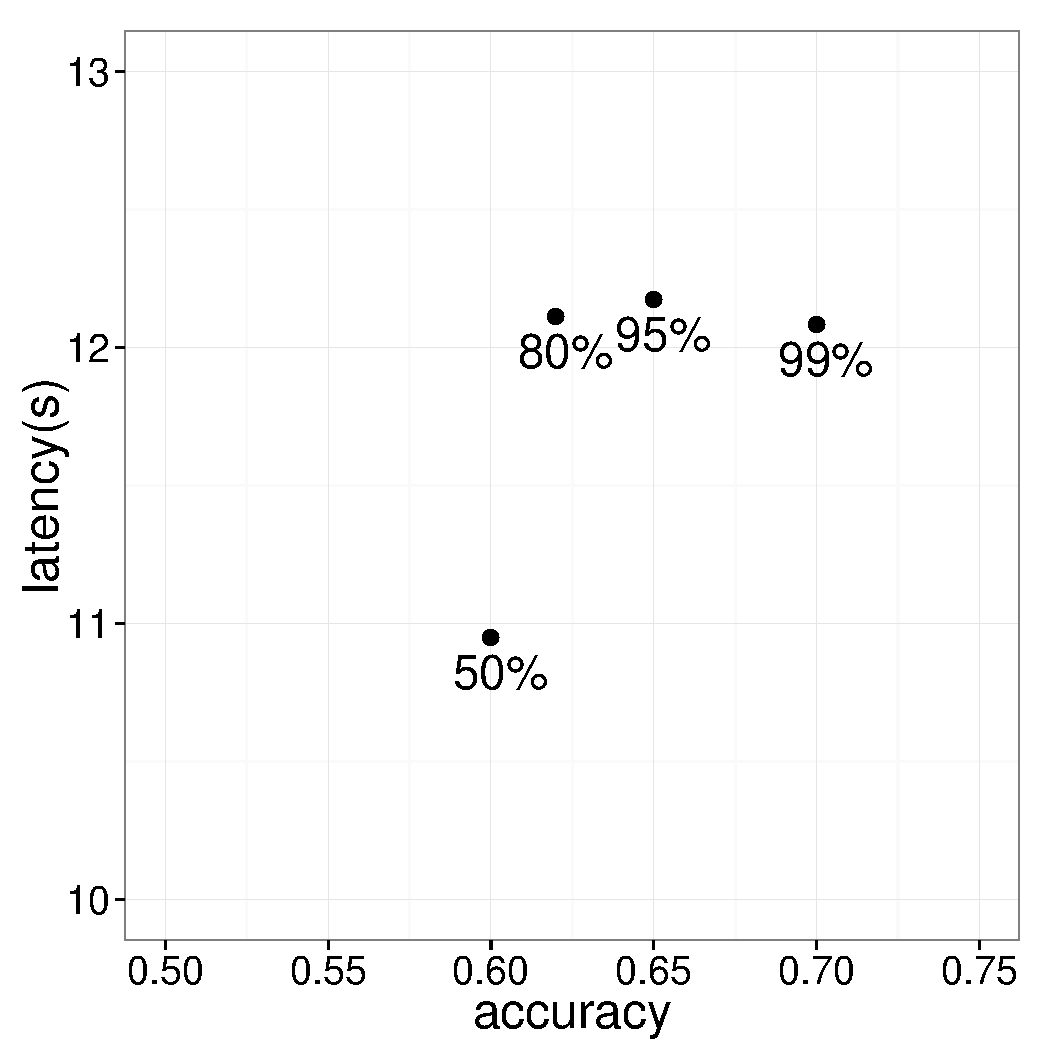
\includegraphics[width=4.2cm] {Images/latency_vs_accuracy_ci.pdf}}
\caption{Latency vs. Accuracy for CI-pruning}
\label{fig:latency_vs_accuracy_ci}
\end{subfigure}
\begin{subfigure}{0.49\linewidth}
\centering
{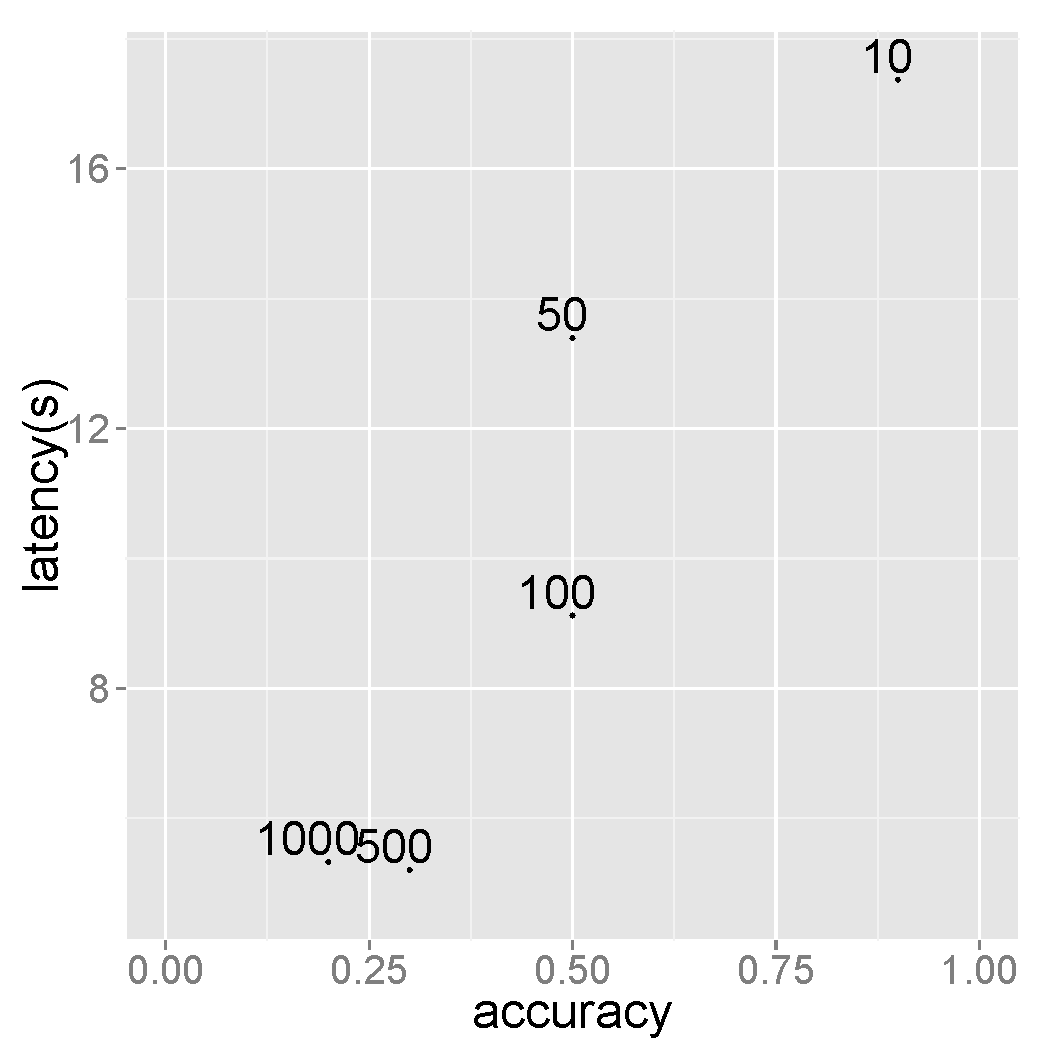
\includegraphics[width=4.2cm] {Images/latency_vs_accuracy_mab.pdf}}
\caption{Latency vs. Accuracy for MAB pruning}
\label{fig:latency_vs_accuracy_mab}
\end{subfigure}
\label{fig:accuracy}
\caption{Latency vs. Accuracy for different heuristics}
\end{figure}

\subsection{Comparison of Execution Engines}

Now that we have examined the performance of both execution engines in detail,
we can make some comparisons across the two execution engines.
As mentioned before, we do not compare the latencies of both engines directly
since the implementations are not directly comparable.
However, we can summarize our findings as follows:
\squishlist
\item In general, column-stores provide better performance on the \VizRecDB\
workload although the workload involves reading every column in a table. This is
likely a consequence of the fact that our individual queries only read a few
columns at a time.
\item For row-stores, the combination of optimizations including combining
multiple aggregates, performing multiple group-bys and running queries in
parallel reduces latency by XXX\%, making \VizRecDB\ interaction possible in
near-interactive times.
\item For column-stores, we saw that the combination of multiple group-bys hurts
performance; however, combining aggregates and running queries in parallel
improves the already good performance of column stores getting response time
down to interactive times.
\item Our heuristics demonstrate that if we are willing to give up a small
amount of accuracy, we can reduce the \VizRecDB\ latency by a factor of 2. We
can also overcome the lower accuracy for small $k$'s by always querying for a
minumum number of views and only returning the top-$k$ views.
\item Finally, we see that if we are able to incorporate our heuristics into an
existing database system as discussed in Section \ref{}, we can expect to
obtain a similar 2X speedup. Along with the optimizations already developed for
the DBMS engine, these heuristics can enable \VizRecDB\ to respond within a
second.
\squishend








%!TEX root=document.tex

\section{User Study}
\label{sec:user_study}

The previous section evaluated \SeeDB 
and our optimizations in terms of performance.
In this section, we assess the utility of \SeeDB's recommendations 
with real users.
First, we perform a study to validate our deviation-based distance metric.
We show that although simple, our deviation-based
metric can find visualizations users feel are interesting.
Second, we compare \SeeDB
to a manual charting tool without visualization recommendations.
We demonstrate that \SeeDB can enable users to find interesting visualizations
faster and can surface unexpected trends.
We also find that users overwhelmingly prefer \SeeDB over a manual charting 
tool.

\subsection{Validating Deviation-based Utility}
\label{sec:validating_metric}

\SeeDB uses deviation between the target and reference dataset as a measure
of interestingness of a visualization.

\stitle{Ground Truth.}
To validate deviation as a utility metric, we obtained ground truth data about
interestingness of visualizations and evaluated \SeeDB against it.
To obtain ground truth, we presented 5 data analysis experts with the Census 
dataset (Section \ref{sec:introduction}) the analysis task of
studying the effect of marital status on socio-economic indicators.
We presented experts with the full set of potential aggregate visualizations 
and asked them to classify each visualization as interesting or
not interesting {\em in the context of the task}.
Of the 48 visualizations, on average, experts classified 4.5 visualizations
(sd = 2.3) as being interesting for the task.
The small number indicates that of the entire set of potential visualizations, 
only a small fraction (\textasciitilde10\%) show interesting trends.
To obtain consensus on ground truth, we labeled
any visualization chosen by a majority of participants as 
interesting; the rest were not. 
This process identified 6 interesting and 42 uninteresting visualizations.
In addition to Figures~\ref{fig:interesting_viz} (interesting) and Figure 
\ref{fig:uninteresting_viz} (not interesting), Figure~\ref{fig:huhi} 
was labeled as interesting (according to a user: ``\ldots it
shows a big difference in earning for self-inc adults'') while 
Figure~\ref{fig:luli} was labeled as not interesting (notice the lack of deviation).
While some classifications can be explained using deviation, some cannot: 
Figure \ref{fig:huli} shows high deviation but was deemed to be uninteresting, 
while Figure \ref{fig:luhi} shows small 
deviation but was deemed to be interesting (``\ldots hours-per-week seems like a 
measure worth exploring''). 

% Figure \ref{fig:gt_examples} shows ground truth for four other visualizations: 
% Figure \ref{fig:huhi} shows another visualization that was chosen as interesting by 4 of 5 
% participants.
% According to participants, this visualization was interesting because ``\ldots it
% showed a big difference in earning for self-inc adults'' and indicated a trend to 
% be examined further.
% Figure \ref{fig:luli} in contrast shows a visualization that participants
% did not select as relevant.
% Notice that the two distributions in this chart do not show significant difference. 
% However, this is not to say that deviation was the only factor relevant for interestingness.
% Figure \ref{fig:huli}, for example, shows a visualization that in fact has high deviation, but was 
% not classified as interesting by any participants.
% Similarly, Figure \ref{fig:luhi} shows a visualization that shows less deviation but was 
% classified as interesting by 2 participants because the .

% The gold standard for evaluating a recommendation system is to obtain ground 
% truth about user preferences about
% various (ideally all) items and examine whether the system's recommendations 
% can correctly classify each item\cite{??}.
% We adopt the same evaluation strategy.
% For the census dataset and associated analytical task (discussed in Section 
% \ref{sec:introduction}), we obtain ground truth about the interesting-ness of 
% each potential visualizations of the dataset.
% We then evaluate whether \SeeDB can correctly classify visualizations as
% interesting or not interesting.

% \stitle{Obtaining Ground Truth}.
% To obtain ground truth, we recruited 5 participants with significant data analysis 
% experience (3 female, 2 male).
% We presented each participant with the Census dataset and the task of finding visualizations
% that showed interesting trends related to marital status (Section \ref{sec:introduction}).
% Participants were presented with the entire set of aggregate visualizations \mpv{how many}
% for this dataset and asked to classify visualizations as being interesting or 
% not-interesting for the task.
% Participants were also asked to explain verbally why they thought a visualization
% was interesting.
% We capped the study at 10 minutes.

\begin{figure}[t]
	\centering
	\begin{subfigure}{0.45\linewidth}
		{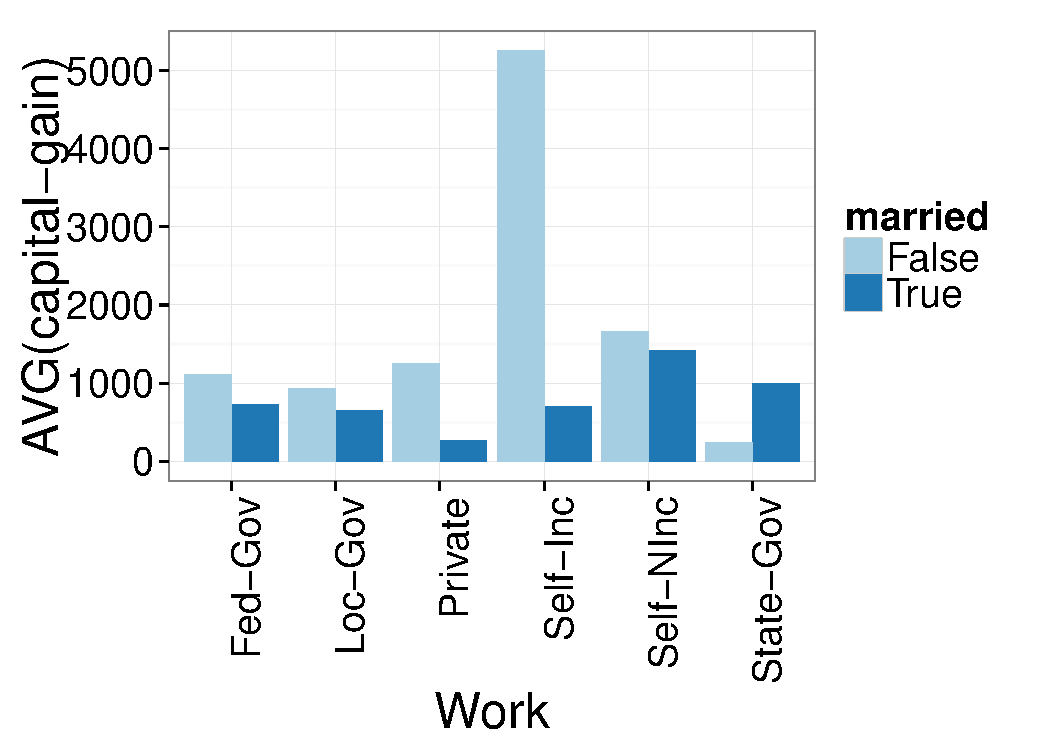
\includegraphics[width=4cm, trim=0 0 3cm 0, clip=true] {Images/HUHI_work_avg_cap_gain.pdf}}
		\caption{High deviation, interesting}
		\label{fig:huhi}  
	\end{subfigure}
	\begin{subfigure}{0.54\linewidth}
		{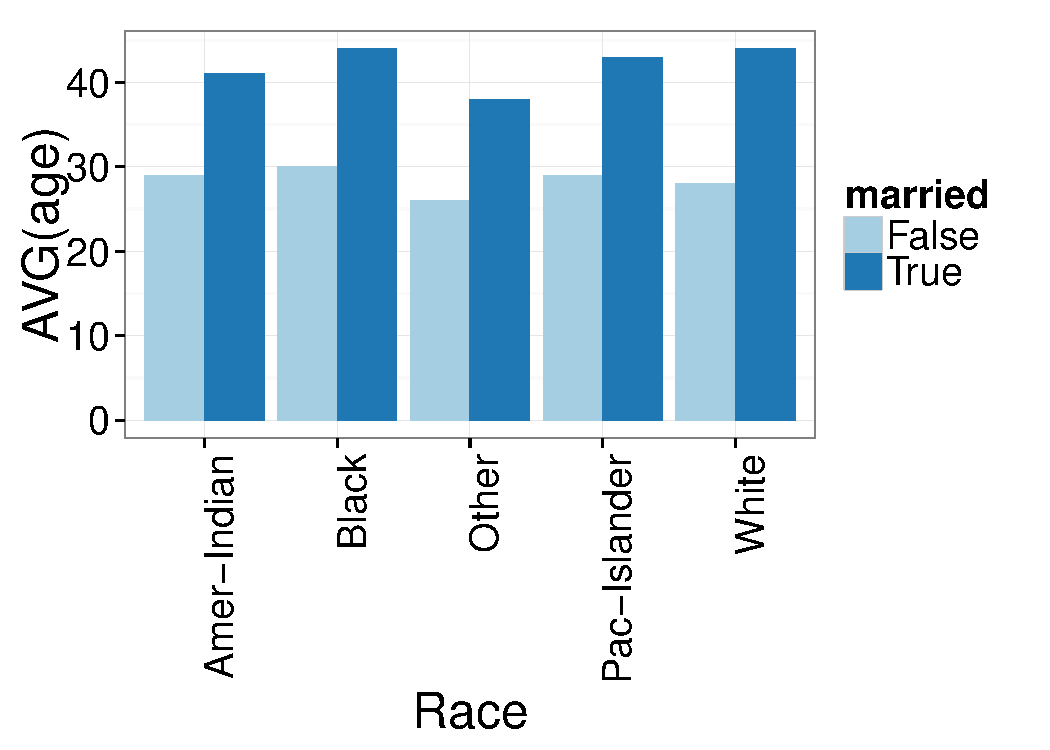
\includegraphics[width=4.5cm] {Images/LULI_race_avg_age.pdf}}
		\caption{Low deviation, not interesting}
		\label{fig:luli}
	\end{subfigure}
	\begin{subfigure}{0.45\linewidth}
		{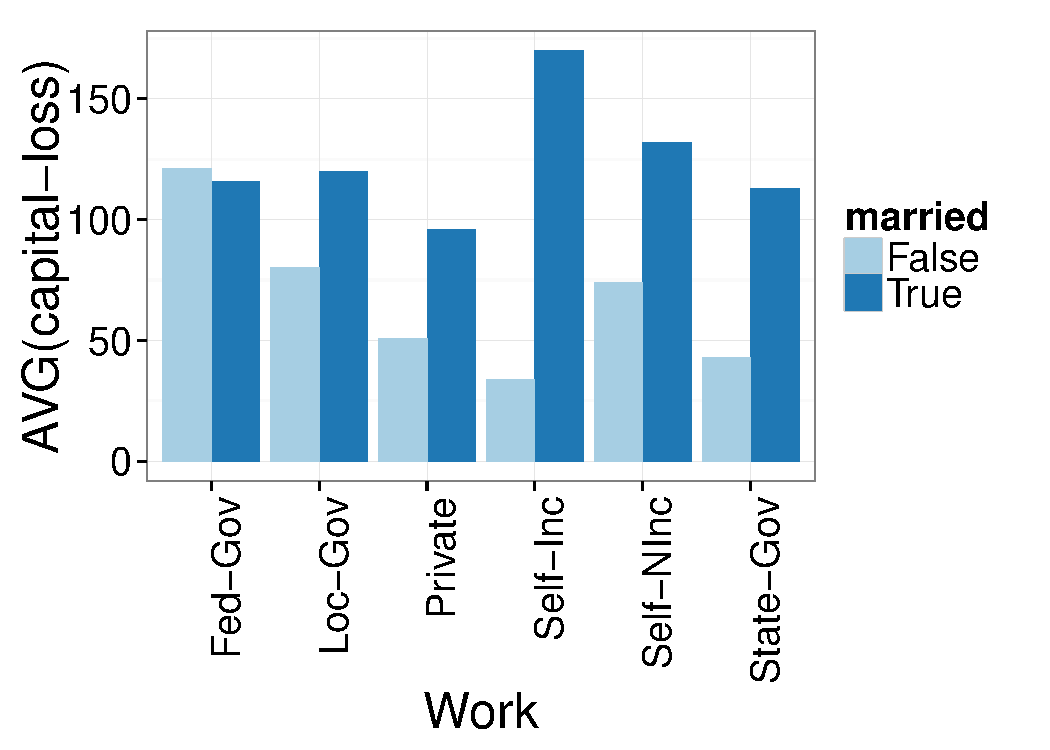
\includegraphics[width=4cm, trim=0 0 3cm 0, clip=true] {Images/HULI_work_avg_cap_loss.pdf}}
		\caption{High deviation, not interesting}
		\label{fig:huli}  
	\end{subfigure}
	\begin{subfigure}{0.54\linewidth}
		{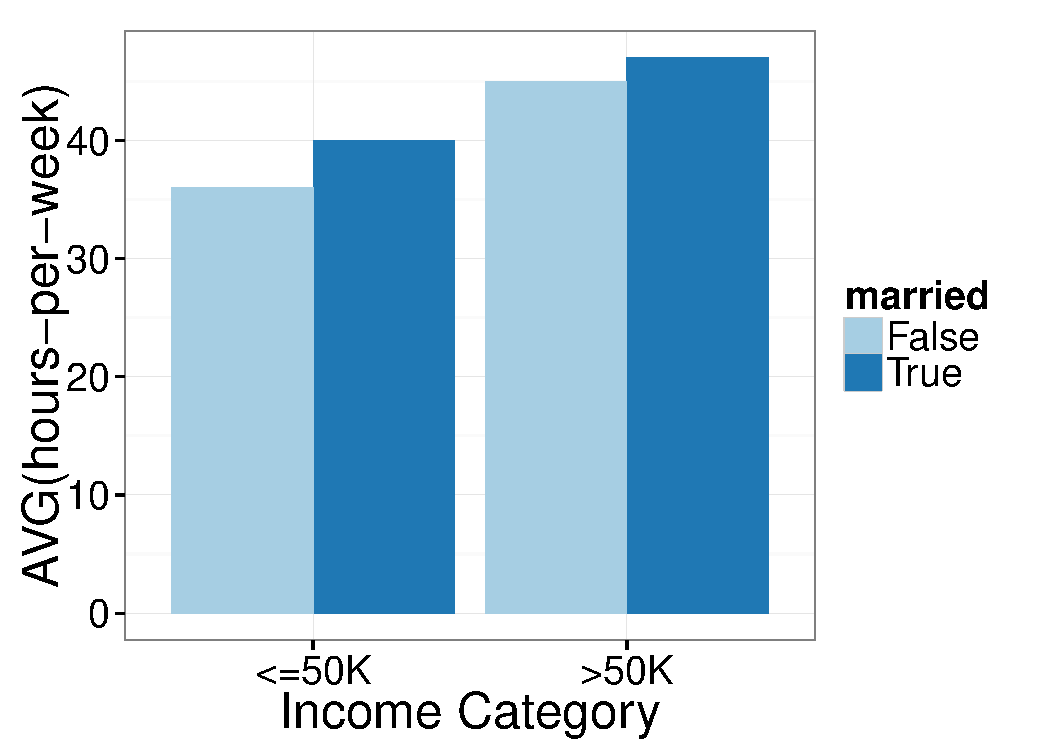
\includegraphics[width=4.5cm] {Images/LUHI_inc_avg_hours.pdf}}
		\caption{Low deviation, interesting}
		\label{fig:luhi}
	\end{subfigure}
	\vspace{-10pt}
	\caption{Examples of ground truth for visualizations}
	\vspace{-10pt}
	\label{fig:gt_examples}
\end{figure} 


% Figure \ref{fig:interesting_viz} in Section \ref{sec:introduction} (showing variation in
% average capital gain across sex for the single and married adults) was a visualization 
% classified as interesting by 4 or 5 participants. 
% In contrast, Figure \ref{fig:uninteresting_viz} was a visualization unanimously classified
% as uninteresting.

% Once we obtained ground truth, we evaluated whether \SeeDB could correctly
% classify visualizations with respect to ground truth.
% In all, participants selected 23 unique visualizations as being interesting.
% To obtain a consensus on ground truth, we used a simple voting system.
% Any visualization that was chosen by majority of participants (3 or more)
% was considered to be interesting; the rest were not.
% Of the 23 unique visualizations classified as interesting, majority of participants 
% agreed on 6 visualizations as being interesting.
% Observe that while there are subjective differences in the criteria for interesting-ness,
% it is possible to distill general criteria for interesting-ness of visualizations.

\begin{figure}[t]
	\centering
	\begin{subfigure}{0.32\linewidth}
		{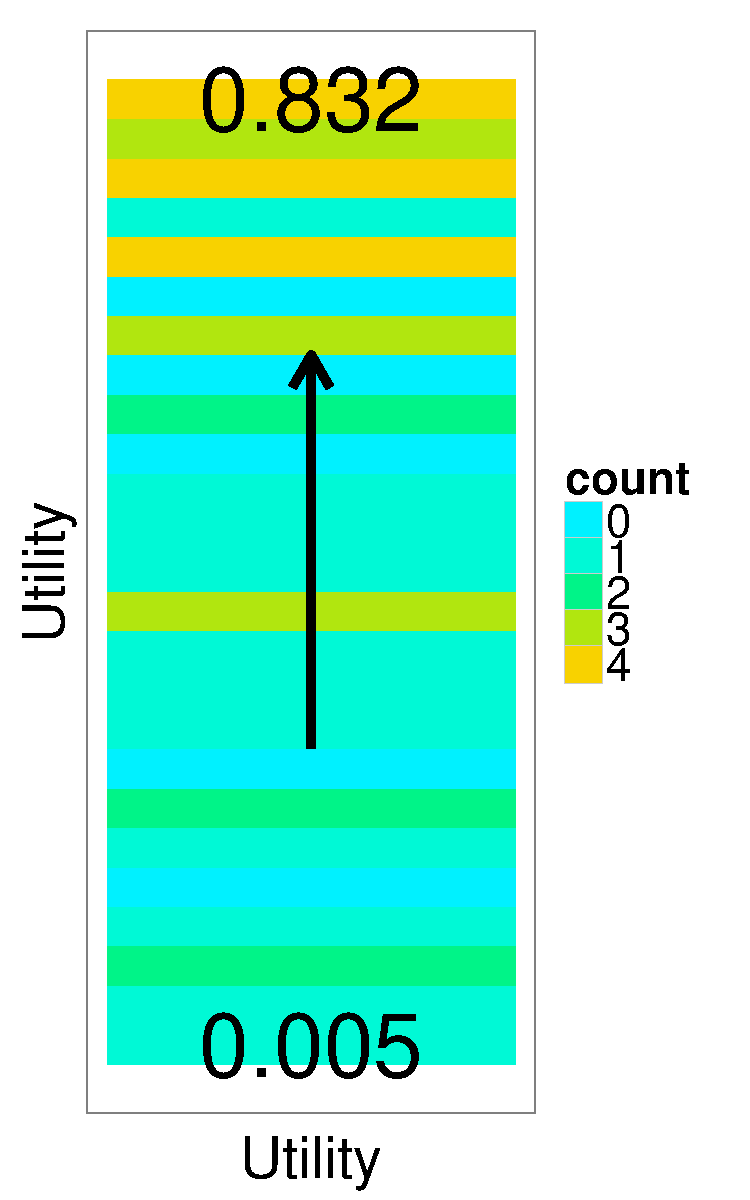
\includegraphics[trim={0 1.3cm 0 0}, clip, width=2.5cm]{Images/census_gt_distribution.pdf}}
		\caption{Utility Distribution}
		\label{fig:gt_dist}
	\end{subfigure}
	\begin{subfigure}{0.65\linewidth}
		\centering 
		{\includegraphics[width=4cm] {Images/seedb_roc.pdf}} 
		\caption{ROC of SeeDB (AUROC = 0.903)}
		\label{fig:roc}
	\end{subfigure}
	\vspace{-10pt}
	\caption{Performance of Deviation metric for Census data}
	\vspace{-20pt}
	\label{fig:census_gt}
\end{figure}

\stitle{Efficacy of Deviation-based Metric}.
Figure \ref{fig:gt_dist} shows a heatmap of the number of times a
visualization was classified as interesting 
({\em yellow} = popular, {\em blue} = not popular), sorted
in {\em descending order} of our utility metric.
We notice that the majority of yellow bands fall at the top of the
heatmap, indicating, qualitatively, that popular visualizations have higher utility.
To evaluate the accuracy of \SeeDB's recommendations over the Census data, 
we ran \SeeDB for the study task, varying $k$ between 0 \ldots 48, and measured
the agreement between \SeeDB recommendations and ground truth.
As is common in data mining, 
we computed the ``receiver operating curve'' or ROC curve for \SeeDB, 
Figure \ref{fig:roc}, depicting 
the relationship between the true positive rate (TPR) on the 
x-axis and false positive rate (FPR) on the y-axis for different values of a
parameter ($k$ in this case). 
TPR is the number of interesting visualizations returned as a fraction of the 
total number of interesting visualizations, 
while FPR is the fraction of recommendations
that were incorrectly returned as interesting, as a fraction of the number
of interesting visualizations returned. 
ROC curves for highly accurate classifiers are skewed towards the upper left
corner of the graph. The red line indicates the random baseline (every example
is classified randomly).
As can be seen in the figure, \SeeDB performs significantly better than the baseline.
For example, for $k$=3, all 3 visualizations recommended by \SeeDB are interesting,
giving TPR = 0.5 and FPR = 0; for $k$=5, 
four of the 5 recommended visualizations are interesting, 
giving TPR = 4/6 = 0.667 and FPR = 0.05. 
The area under ROC (AUROC) for \SeeDB---the typical measure of 
classifier quality---is 0.903.
This indicates that the accuracy of \SeeDB recommendations is very high.\footnote{\small AUROC's 
above 0.8 are considered very good, while those above 0.9 are
excellent}
%\mpv{add points on chart for k=3, 5}

While ROC curves on different datasets and tasks will vary,
this user study shows that \SeeDB recommendations have high quality
and coverage,
despite focusing on a simple deviation-based utility metric.
We expect that taking into account other aspects (apart from deviation),
would improve \SeeDB's recommendations even more.

% We varied the number of visualizations $k$ recommended by \SeeDB between 0 and
% max \mpv{fill in max}.
% For each value of $k$ we computed the number of true positives (\SeeDB recommended
% visualizations that were classified as ``interesting'' by majority), false
% positives, true negatives and false negatives.
% The true positive rate (recall) and false positive rate for \SeeDB are shown 
% in the `receiver operating curve'' (ROC)\cite{} in Figure \ref{fig:roc}.
% As expected, we observe that as $k$ increases, the true positive rate (TPR)
% increases (or stays constant), but false positive rate (FPR) also increases as 
% more visualizations are incorrectly classified as interesting.
% Clearly, \SeeDB performs significantly better than the baseline algorithm which 
% classifies every visualization as interesting with 50\% probability.
% For example, for $k$ = 3, TPR = 0.5 and FPR = 0;
% i.e., for $k$ = 3, all 3 visualizations recommended by \SeeDB are in fact interesting.
% However, \SeeDB recovers only 3 of the 6 visualizations.
% Likewise, for $k$ = 5, 4 of 5 of the recommended visualizations are interesting, giving
% TPR = 0.667 and FPR = 0.05.
% Finally, for $k$=14, \SeeDB recommends all 6 interesting visualizations, giving a 
% TPR of 1 but having an FPR of 0.421.
% The standard metric for computing quality of a recommender is to
% compute AUROC or area under the ROC curve.
% AUROC for \SeeDB in \ref{fig:roc} is 0.903.
% AUROC values above 0.8 are indicative of
% high quality of recommendations \cite{}, demonstrating that \SeeDB performs very well in
% making recommendations.

% While ROC curves for \SeeDB will vary with dataset and query, the above analysis, both
% qualitatively and via ROC, indicates that our deviation-based metric can in fact identify
% interesting visualizations with high accuracy.
% Although there are many other factors that determine interesting-ness, deviation seems
% to capture a significant part of the metric. 

% Now that we have validated our deviation-based metric, we examine how \SeeDB, a visualization tool
% with deviation-based recommendations, compares to a manual chart construction tool in performing
% visual analysis.

\subsection{{\large \SeeDB} vs. Manual Visualization Tool}
\label{sec:seedb_vs_manual}

The motivation behind \SeeDB is to build a tool that can support fast
visual analysis by automatically recommending interesting visualizations.
In this section, we describe results from a controlled user study comparing 
\SeeDB to a manual visualization tool for performing visual analysis. 
We hypothesized that: (i) when using \SeeDB, analysts would find interesting 
visualizations {\em faster} than when using the manual tool, (ii) analysts
would find {\it more} interesting visualizations when using \SeeDB vs. the 
manual tool, and (iii) analysts would {\em prefer} using \SeeDB to a manual tool.

% Next, we assess the efficacy of \SeeDB in enabling fast visual analysis.
% Towards this, we 
% To assess the efficacy of \SeeDB in enabling faster visual analysis,
% we conducted a user study where participants performed visual analysis
% using both \SeeDB and a manual chart construction tool.
% We hypothesized that: (i) When using \SeeDB, participants would find 
% interesting visualizations {\em faster} than when using manual chart
% construction, (ii) Participants would find more interesting visualizations
% when using \SeeDB vs. when using manual chart construction, (iii) 
% Participants would prefer using a tool with recommendations vs. a manual
% construction tool.

\stitle{Participants and Datasets}. We recruited 16 participants (5 female, 11
 male) all graduate students with prior data analysis experience and visualization
 experience (e.g. R, matplotlib or Excel).
 None of the participants had previously worked with the study datasets.

 Our study used the Housing and Movies datasets from 
 Table \ref{tab:datasets}.
 These two datasets were chosen because they were easy to understand and 
 were comparable in terms of size and number of potential visualizations.
 
\stitle{Study Protocol}.
Our study used a 2 (visualization tool) X 2 (dataset) within-subjects design.
The visualizations tools used were \SeeDB and {\em MANUAL}, a manual chart
construction-only version of \SeeDB (i.e., \SeeDB with the recommendations bar, 
component ``D'' in Figure \ref{fig:frontend1}, removed).
Using the same underlying tool in both modes allowed us to control for
tool functionality and user interface.
We used a within-subjects design to compensate for per-participant differences 
in data analysis expertise, and used counterbalancing to remove any effects 
related to order and the test dataset.

Our study began with a short tutorial on the two study tools.
Following the tutorial, participants were asked to perform two visual analysis 
tasks, one with \SeeDB in each mode.
For each mode, we introduced participants to the test dataset
and the analytical prompt using written instructions.
Each analytical task asked participants to use the specified tool to find 
visualizations supporting or disproving a specific hypothesis.
Participants were asked to use the bookmark button (in component ``C'' in Figure 
\ref{fig:frontend1}) to flag any visualizations they deemed interesting in
context of the task.
Participants were also encouraged to think aloud during the study.
Since the analytical tasks were open-ended, we capped each analysis session at 8 minutes.
Participants filled out a tool-specific survey at the end of each task and
an exit survey at the end of the study.
Most survey questions were answered on a 5-point Likert scale.
The study lasted \textasciitilde 45 minutes and participants were compensated 
 with a \$15 gift card.
All studies were conducted in a lab setting using Google Chrome on a 15-inch 
Macbook Pro.

\stitle{Methods and Metrics}.
Over the course of each study session, we collected data by three means: interaction logs 
from each tool, responses to surveys, and exit interview notes.
The interaction logs capture the number of visualizations
constructed, the number of visualizations bookmarked, bookmark rate, and interaction traces.
\SeeDB and MANUAL both support the construction of different types of charts such as bar 
charts, scatterplots etc.
Since \SeeDB can only recommend aggregate visualizations shown as bar charts,
we report results for aggregate visualizations.
We evaluate statistical significance of our results using paired t-tests and ANOVA,
and supplement interaction analysis with qualitative data from surveys and study notes.


% Since users were asked to bookmark visualizations they found to be relevant to the task,
% bookmarking behavior from tool interaction logs provides a rich source
% of information about the analytical process.
% Specifically, we study a number of metrics including: (i) number of bookmarks ($num\_bookmarks$), 
% (ii) total number of visualizations viewed ($total\_viz$), 
% (iii) bookmarking rate ($bookmark\_rate$) defined as $num\_bookmarks$/$total\_viz$, and 
% (iv) the time between consecutive bookmarks ($bookmark\_time$).
% \SeeDB and MANUAL support construction of two kinds of charts: aggregate visualizations and 
% scatterplots (to replicate real visual analysis).
% Since \SeeDB can only recommend aggregate visualizations, we also analyze the above
% metrics for aggregate visualization only.
% We supplement bookmark analysis with qualitative data from surveys and study notes.
% We evaluate statistical signifance of our results using paired t-tests and ANOVAs.

\stitle{Results}.
Over the course of our study, participants built over 220 visualizations 
and bookmarked 70 visualizations.
The overall bookmark rate was 0.32.
We next describe our key findings and observations.

\stitle{1. \SeeDB enables fast visual analysis}.
Table \ref{tab:agg_bookmarks} shows an overview of the bookmarking behavior for each tool
focusing on total number of visualizations generated, number of bookmarks and bookmarking rate.
First, we observe that the total number of (aggregate) visualizations created in the \SeeDB
condition is higher than that for MANUAL. 
While not statistically significant, this difference suggests that analysts are exposed to more
{\em views} of the data with \SeeDB than MANUAL, possibly aiding in a more thorough exploration of
the data.
Next, we find that the number of aggregate visualizations bookmarked in \SeeDB is much higher (3X more)
than that for MANUAL.
In fact, the two-factor analysis of variance shows a significant effect of tool on the number of bookmarks,
F(1,1) = 18.609, p < 0.001. 
We find no significant effect of dataset, F(1, 1) = 4.16. p > 0.05, or
significant interaction between tool and dataset.
While this result indicates that analysts bookmark more visualizations in \SeeDB, we note that the number of 
bookmarks for a tool may be affected by the total number of visualizations built with the tool.
Therefore, to account for variance in the total number of visualizations, we also examine $bookmark\_rate$
for the two tools defined as the fraction of
created visualizations that are bookmarked ($\frac{num\_bookmarks}{total\_viz}$).
We find, once again, that the $bookmark\_rate$ for \SeeDB (0.42) is 3X larger than the $bookmark\_rate$ for 
MANUAL (0.14).
The two-factor analysis of variance shows a significant effect of tool on bookmark rate, F(1,1) = 10.034, p < 0.01.
As before, we find no significant effect of dataset on bookmark rate, F(1, 1) = 3.125. p > 0.05, or
significant interaction between tool and dataset.
Together the two results above indicate that there is a {\bf significant effect of tool on both the number of bookmarks as well as the
bookmark rate}.
\SeeDB-recommended visualizations are 3 times more likely to be interesting compared
to manually constructed visualizations.
%In other words, analysts are 3X more likely to arrive at interesting visualizations
%when using \SeeDB vs. MANUAL:
%\SeeDB can thus allow analysts to find analyze data faster. 
%\mpv{Remove? Finally, we note that the statistical results regarding faster analysis are supported by anecdotal evidence 
%and survey data from study participants.
Finally, 87\% of participants indicated that \SeeDB recommendations sped up their visual analysis, many alluding
to the ability of \SeeDB to ``\ldots quickly deciding what correlations are relevant'' and 
``[analyze]...a new dataset quickly''.


% Moreover, we once again find this difference in $bookmark\_rate$ is statistically significant
% within subjects as well as across subjects ({\em Paired t-test, t = -2.5599, df = 8, p-value = 0.03365}).
% This implies that {\bf a \SeeDB-recommended visualization is 3 times more likely to be
% interesting compared to a manually constructed aggregate visualization}.
% In other words, users are 3X more likely to arrive at interesting visualizations when using
% \SeeDB vs. MANUAL; i.e., \SeeDB can enable users to find interesting insights faster.
% Results of a 2-way ANOVA also indicate that \SeeDB has a significant impact on 
% aggregate bookmark rate ({\em df = 1, sum sq = 0.3681, mean sq = 0.3681, F value = 10.034, p = 0.00685}). 
% (We find that choice of dataset does not affect bookmark rate, and there are no interaction or order effects.)

% We also find that, on average, the $bookmark\_time$ for \SeeDB (92.91 $\pm$ 49.26) is twelve seconds 
% shorter than that for MANUAL (105.02 $\pm$ 58.24). 

% However, unlike in Table \ref{tab:bookmarks}, we observe that number of aggregate visualizations 
% is higher for \SeeDB compared to MANUAL suggesting that the larger number of bookmarks in \SeeDB 
% might be a consequence of a larger number of aggregate visualizations with \SeeDB (possibly because
% \SeeDB only recommends aggregate visualizations)\footnote{Although \SeeDB only recommends aggregate
% visualizations, users have the ability to plot or modify a recommendation to construct a scatterplot}.
% As a result, we find $bookmark\_rate$, which is the proportion of aggregate visualizations bookmarked
% to the number of aggregate visualizations viewed, to be an unbiased metric.
% We find that $bookmark\_rate$ for \SeeDB (0.42) is in fact 3X larger than the $bookmark\_rate$ for 
% MANUAL (0.14).
% This implies that \stitle{a \SeeDB recommended aggregate visualization is 3 times more likely to be
% interesting compared to a manually constructed aggregate visualization}.

% A 3X higher $bookmark\_rate$ implies that users are 3X more likely to find interesting insights with 
% recommended visualizations vs. if they create visualizations manually; i.e., \SeeDB can enable users 
% to find interesting insights faster.

\begin{table}[htb]
  \centering \scriptsize
   \vspace{-5pt}
  \begin{tabular}{|c|c|c|c|c|} \hline
   & total\_viz & num\_bookmarks & bookmark\_rate \\ \hline
  MANUAL & 6.3 $\pm$ 3.8 & 1.1 $\pm$ 1.45 & 0.14 $\pm$ 0.16 \\ \hline
  \SeeDB & 10.8 $\pm$ 4.41 & 3.5 $\pm$ 1.35 & 0.43 $\pm$ 0.23 \\ \hline
  \end{tabular}
  \vspace{-10pt}
  \caption{Aggregate Visualizations: Bookmarking Behavior Overview}
  \label{tab:agg_bookmarks} 
  \vspace{-5pt}
\end{table}



% We find that, in general, participants bookmarked slightly more visualizations with \SeeDB than 
% with MANUAL.
% On the other hand, we find that participants interacted with fewer visualizations in \SeeDB than
% in MANUAL.
% As a consequence of these two opposing forces, we find that participants using \SeeDB view fewer
% visualizations but bookmark more, i.e., the visualizations they interact with are, on average, 
% higher quality.
% This trend id reflected in the $bookmark\_rate$ for \SeeDB; the $bookmark\_rate$ for \SeeDB is 1.5X 
% higher than that for MANUAL.

% While these differences are not statistically significant, they point towards a trend: {\it \SeeDB
% enables participants to arrive at interesting visualizations faster than MANUAL}.

% \begin{table}[htb]
%   \centering \scriptsize
%   \begin{tabular}{|c|c|c|c|c|} \hline
%    & num\_bookmarks & total\_viz & bookmark\_rate \\ \hline
%   MANUAL & 3.3 $\pm$ 1.42 & 14.1 $\pm$ 5.4 & 0.24 $\pm$ 0.09 \\ \hline
%   \SeeDB & 3.5 $\pm$ 1.35 & 12.1 $\pm$ 4.7 & 0.36 $\pm$ 0.22 \\ \hline
%   \end{tabular}
%   \vspace{-10pt}
%   \caption{All Visualizations: Bookmarking behavior Overview}
%   \label{tab:bookmarks} 
%   \vspace{-10pt}
% \end{table}



% Recall that \SeeDB (currently) only supports recommendations for aggregate visualizations.
% The above results include data for both scatterplots as well as aggregate visualization, and
% therefore do not entirely reflect bookmark behavior for aggregate visualizations.
% Table \ref{tab:agg_bookmarks} shows the same bookmarking metrics as in Table \ref{tab:bookmarks}
% for aggregate visualizations.

\stitle{2. All participants preferred \SeeDB to MANUAL}. 
The most important result of our survey was that 100\% of all users preferred \SeeDB to MANUAL for
visual analysis, i.e., all users preferred to have recommendation support during analysis.
78\% of participants found the recommendations ``Helpful'' or ``Very Helpful'' and thought that they
showed interesting trends.
In addition, majority of users found \SeeDB a powerful means to get an overview of interesting trends
and starting points for further analysis. 
One participant noted that \SeeDB was ``\ldots great tool for proposing a set of initial queries for a dataset''.
Due to space constraints, we explore this result further in the associated tech report~\cite{seedb-tr}.
77\% of participants also indicated that \SeeDB visualizations showed unexpected trends (e.g. big difference
in capital gain for Self-Inc in Figure \ref{fig:huhi}), and indicated that \SeeDB suggested visualizations
they wouldn't have created,
e.g. ``\ldots interesting aspects of data to compare. I don't think I would have checked those by myself.''.
% To illustrate, Figure \ref{blah} \mpv{making these} shows two visualizations that were not generated by participants using MANUAL,
% but were in fact recommended by \SeeDB\ {\it and} bookmarked as being interesting.
%\papertext{An intriguing observation we made was that while some analysts liked having recommendations, 
%they did not want to rely 
%too heavily on recommendations but instead let intuition guide their analysis.}
\techreport{An intriguing observation from two participants was that while they wanted recommendations to support them
in analysis, they did not want to rely too heavily on recommendations and ignore their creativity.
One participant noted {\em ``The only potential downside may be that it made 
me lazy so I didn't bother thinking as much about what I really could study or be interested in''}.
This observation suggests lines for future work that can find the right balance between automatically 
recommending insights and allowing the user to leverage their intuition and creativity.}

\techreport{
\begin{figure}
	\centering
	{\includegraphics[trim={0 0 0 0}, clip, width=9cm]{Images/traces.pdf}}
	\caption{Interaction trace examples: (R) = Recommendation, (M) = Manual, (B) = Bookmark}
	\vspace{-10pt}
	\label{fig:traces}
\end{figure}

\stitle{3. \SeeDB provides a starting point for analyses}. 
To our knowledge, \SeeDB is the first tool to provide recommendations for supporting visual
analysis.
As a result, we were interested in how recommendations could fit into the analytical workflow.
While a participant's exact workflow was unique, we repeatedly found specific patterns in the
interaction traces of \SeeDB.
Figure \ref{fig:traces} shows examples of three such traces.
Interaction traces show that participants often started with a recommended visualization, 
examined it, modified it one or more times (e.g. by changing to a different aggregate function 
or measure attribute) and bookmarked the resulting visualization.
%  {\em recommendation 
% $\rightarrow$ manual\_modify $rightarrow$ manual\_modify $rightarrow$ \ldots bookmark}.
% Specifically, participants would often start from one of the recommendations and explore other
% visualizations that were variations of it (e.g. different aggregation or measure attribute) 
% until they found an interesting visualization.
% \mpv{can I put any data here?}
Thus, even if participants did not bookmark recommendations directly, their often created
small variations of the visualization and bookmarked them.
In other words, along with providing recommendations that were interesting by themselves, \SeeDB
helped direct participants to other interesting visualizations by {\em seeding} their analysis.
This pattern was highlighted in user comments as well; e.g.,
``\ldots would be incredibly useful in the initial analysis of the data'', 
``\ldots quickly deciding what correlations are relevant and gives a quick peek'',
``\ldots great tool for proposing a set of initial queries for a dataset''.
In addition to understand the role recommendations played in analysis, these observations 
also serve to reinforce the design choice of \SeeDB as a complement to a traditional
visualization system vs. a standalong system; the mixed-initiative nature of the tool 
is essential for it to be functional in visual analysis.
}


\techreport{
\subsection{Limitations}
Given that both studies described above were conducted in the lab, the studies had limitations.
First, due to constraints on time and resources, the sample sizes for both studies were small.
A larger set of participants and spread of datasets could be used to further demonstrate the
efficacy of our system.
Second, our user studies were conducted with graduate students participants who, on one hand, 
likely have higher data analysis skills than typical users, while on the other hand, are 
not experts in the dataset being analyzed.
Consequently, our results represent results the perspective of capable data analysts who 
have limited familiarity with the data.
We find that \SeeDB is particularly well suited for this particular setting of initial data 
analysis when the user is not very familiar with the data (\~ coldstart).
It would be instructive to evaluate \SeeDB on datasets about which users have expert knowledge.
Finally, we note that being a research prototype, limited functionality of \SeeDB (e.g. in types of
charts) and potential issues with learnability and interactivity may have also had an impact on
our study.

\mpv{Also: The datasets we evaluated had a relatively small (< 100) number of potential visualizations;
it would be valuable to evaluate the performance of \SeeDB on datasets with thousands of potential
visualizations.
It is also possible that some datasets were easier to interpret than others.
}
}



% 86\% of participants indicated that the recommendations sped up their analysis.


% When asked to rate the recommendations provided by \SeeDB, 78\% participants indicated that the
% recommendations were either ``Helpful'' or ``Very Helpful''. 
% We also found that 90\% of participants found the comparative visualizations shown by \SeeDB 
% helpful in their analysis.
% 66\% of participants indicated that the recommendations needed improvement, in particular,
% participants were interested in seeing different types of charts (e.g. geographical, time series)
% and obtaining measures of statistical significance.

% \stitle{Qualitative Feedback}. In their qualitative feedback, participants highlighted the importance of 
% a tool like \SeeDB at the initial stages of analysis. 
% One partitipant said, {\em ``It's a great tool for proposing a set of initial queries for a dataset I have never seen. 
% And from these visualizationns, I can figure out which related patterns to dig into more.''}
% Others thought that the strength of the tool was in quickly finding relevant trends, {\em ``It's a good tool that helps 
% in quickly deciding what correlations are relevant and gives a quick peek''}. 
% Overall, participants indicated that \SeeDB was particularly suited for exploratory analysis of new datasets, 
% {\em ``I thought SeeDB was very helpful in helping me get more familiar with a new dataset quickly.''}.




 %!TEX root=document.tex
\techreport{
\section{Convergence of Utility Metrics}
\label{sec:convergence}

\stitle{Convergence of Sampling Algorithms.}
We now demonstrate how,
when applied to the utility function $U$ as described
in Section~\ref{sec:problem_statement},
sampling algorithms 
converge to the correct value of $U$ beyond a certain number of samples.

For now, we focus on the case where the visualization $V_i$
corresponds to the AVG aggregate. 
Similar results can be shown for the SUM and STD
aggregates. 
Unfortunately, MAX and MIN are not amenable to sampling-based
optimizations, as is traditionally well-known in the approximate
query processing literature~\cite{wavelets,dbo}.

Additionally, we focus on the case when $S$ is defined to be
$\ell_2$, i.e., the Euclidean distance metric. 
Once again, similar results can be shown for other distance metrics,
such as the $\ell_1$, the Earth Movers Distance metric, or
the Jenson-Shannon metric.

We reproduce the utility equation here:
$ U (V_i) = S ( P[V_i (D_Q)], P[V_i (D)] )$.
Here, $P$ refers to the probability distribution
of either the target visualization
or the comparison visualization.
$P$ is represented as a normalized vector
whose entries sum up to $1$.
We have the following: 
\papertext{(The proof can be found in the extended technical report~\cite{seedb-tr}.)}
\begin{lemma}
Let the target and comparison visualizations
both have $m$ groups.
Let $\hat{U}$ denote our estimate of $U$ based on a uniformly random sample 
across all $m$ groups. 
Then, as the number of samples tends to $\infty$, $\hat{U} \rightarrow U$
with probability $1-\delta$, for as small $\delta$ as needed.
\end{lemma}
\papertext{At a high level, the proof
involves repeated applications of Hoeffding's inequality to
upper and lower-bound $\hat{U}$ within $U$ along with terms 
that tend to $0$ as the number of samples increases.}
}
\techreport{
\begin{proof} (Sketch)
Let us say the estimated average for the target visualization
for each of the groups is $\hat{t}_i$,
and the estimated averages for the comparison visualization
for each of the groups is $\hat{c}_i$.
We further define $\hat{t}$ (respectively $\hat{c}$) to be the estimated sum of
averages for the target visualization (respectively comparison visualization).
We let the true values for each of these quantities be the same variables without
the hats.
Then, it can be shown that that $U$ evaluates to:
$$\hat{U} = \frac{\sum{\hc_i^2}}{\hc^2} +  \frac{\sum{\htt_i^2}}{\htt^2} - 2 \frac{\sum{\htt_i \hc_i}}{\hc\htt}$$


Now we informally describe the steps of our proof:
say we sample enough to get $\hc$ within $\epsilon$ of $c$, with a high enough probability,
and we sample enough to get $\htt$ within $\epsilon$ of $t$, with a high enough probability.
Then, we have 
\begin{align*}
\hat{U} & \geq \frac{\sum{\hc_i^2}}{(c + \epsilon)^2} +  \frac{\sum{\htt_i^2}}{(t + \epsilon)^2} - 2 \frac{\sum{\htt_i \hc_i}}{(c - \epsilon) (t - \epsilon)} \\
& \geq \frac{\sum{\hc_i^2}}{c^2} (1 - \epsilon ) +  \frac{\sum{\htt_i^2}}{t ^2} (1-\epsilon) - 2 \frac{\sum{\htt_i \hc_i}}{(c - \epsilon) (t - \epsilon)} \\
& \geq \frac{\sum{\hc_i^2}}{c^2} (1 - \epsilon ) +  \frac{\sum{\htt_i^2}}{t ^2} (1-\epsilon) - 2 \frac{\sum{\htt_i \hc_i}}{ct}(1 + \epsilon^2 + \epsilon) 
\end{align*}
Similarly, if we have sampled enough to get the $\hc_i$ and the $\htt_i$ within $\gamma$ close 
of their actual values, we will have:
\begin{align*}
\hat{U} \geq &  \frac{\sum{c_i^2}}{c^2} (1 + f(\gamma)) (1 - \epsilon ) +   \frac{\sum{t_i^2}}{t ^2}  (1 + f(\gamma)) (1-\epsilon) \\ & - 2 \frac{\sum{t_i c_i}}{ct}(1 + h(\gamma))(1 + \epsilon^2 + \epsilon) 
\end{align*}
where $f(.)$ and $h(.)$ are small polynomial functions.
Thus,
we will have sandwiched $\hat{U}$ from the bottom by $U-\rho$,
and similarly by $U + \rho'$ from the top.
$\rho, \rho'$ will be polynomials that depend on $\epsilon$ and $\gamma$.
Now, we will use the Hoeffding's inequality for the last step of the proof.
Hoeffding's inequality, when
applied to a collection of $n$ i.i.d. random variables,
whose sum is represented by $X$, gives us:
\begin{equation}
Pr (|X - E[X]| \geq t) \leq 2 e^{-\frac{2 n t^2}{c^2}}
\end{equation}
where $c$ is a bound on the range. 
If we set the right hand side to some $\delta$, and set $t = \epsilon$,
we have
$$ \epsilon = \sqrt{\frac{1}{2 n} \ln \frac{2}{\delta}}$$
and therefore, as $n$ tends to $\infty$, $\epsilon$ tends to $0$,
for fixed values of $\delta$.
The same holds true for $t = \gamma$.
Thus, $\hat{U}$ will tend to $U$ as the number of samples
increases to infinity.
\end{proof}

It is in fact also possible to explicitly derive a number of samples 
such that $\hat{U}$ is close to $U$ within a certain error bound
and with a certain probability. 
}



\section{Extensions}
\label{sec:discussion}

\subsection{Extension to other Utility Metrics}
\label{sec:other_utility_metrics}

\subsection{Comparison of Different distance Metrics for Deviation}
\label{sec:diff_dist_metrics}
\mpv{something goes here}

\subsection{Metrics other than deviation}

% In this section we prove that our sampling 
% algorithms converge, and then describe our generalized
% distance metric.

In Section \ref{sec:introduction}, we introduced a set of {\it dimensions} that determine the quality of a visualization.
In subsequent sections, we developed a system that used metadata, data distributions, and the input query
to recommend visualizations based on deviation.
In this section, we discuss how our deviation metric can encompass a variety of distribution-based metrics and how we can augment our system to take other quality dimensions into account.

First, consider an extension of the utility function $U (V_i)$ denoted as $f_D (V_i)\ =\ w_d \times S_d + w_h \times S_h + w_l  \times S_l$.
Here, the first component corresponds to the utility definition from Section~\ref{sec:problem_statement}
so that $S_d = S ( P[V_i (D_Q)],$ $P[V_i (D)] )$ takes into account the deviation between the data selected by the query and the comparison data.
We can use the same distance metric $S$ to also capture utility based on historical context. 
For instance, let $S_h = S ( P[V_i (D_Q)], $ $P[V_i (D_C)] )$ where
$P[V_i (D_C)]$ refers to the typical value of the distribution 
$P[V_i (D_Q)]$, given historical data.
For instance, when $V_i$ refers to sales of a particular chair in 
Boston, $V_i(D_C)$ could be sales of that chair in Boston for the past 10 years.
% This measure would then allow us to identify whether the value for particular sales is 
% deviating significantly from past patterns and is therefore interesting.
Finally, we can also use the deviation-based metric to capture local trends.
For instance, let $S_l = S ( P[V_i (D_Q)], P'[V_i (D_Q)] )$ where
$P'[V_i (D_Q)]$ refers to the distribution $P$, but shifted slightly.
For instance, if the sensor readings in the last five minutes differ greatly
for current readings, the utility of $V_i$ would be high.
This component can capture
the amount of rapid local changes that have happened
within the distribution corresponding to $P[V_i (D_Q)]$.
A combination of the above deviation-based metrics provides a rich model to capture a large
portion of distribution-based utility.

Next, we turn to the question of incorporating other recommendation dimensions into our utility 
metric.
Recall from Section \ref{sec:introduction} that along with metadata, query and distribution (the
dimensions supported by our metric), other recommendation dimensions include aesthetics, user
preferences and semantics.
Consider the following form of a generalized utility function:
$$ U (V_i) = f_{MA}(V_i) \times f_P (V_i) \times f_D (V_i)$$

Let $f_D (V_i)$ be the utility function measuring distribution-based utility of $V_i$.
We can then augment $f_D (V_i)$ with $f_{MA}(V_i)$ and $f_P (V_i)$ capturing metadata and semantics, and user preferences respectively.
For instance, $f_{MA}(V_i)$ can capture best-practices about visualization and output a utility value accordingly.
Similarly, let $f_P (V_i)$ be a function that models the users' preference towards seeing visualization $V_i$. 
This function can take into account past user history at both the individual and global levels.
For instance, if the analyst typically looks at sales over time, $f_P (V_i)$ for sales over time
may be high.
Similarly, if sales is a popular attribute across all data analysts, $f_P (V_i)$ could be large for
a $V_i$ that depicts sales.
We can also think of $f_P (V_i)$ as capturing in a limited way semantics that can be mined from previous user interactions.
We note however that semantics is one dimension that an automated recommendation system will not be able to capture fully.

In terms of the visualization recommendations, we find that $f_{MA}(V_i)$ and $P (V_i)$ are independent
of the data distribution.
Once a user poses a query, we can merely reuse previously computed values for these functions while
making the recommendation.
For \SeeDB, these functions amount merely to constants in the utility function $U (V_i)$ that would assign weights to each view.
Thus, in this form, we find that \SeeDB can easily incorporate other recommendation dimensions into
the utility metric without any changes to the \SeeDB framework.

% Let $f_{MA}(V_i)$ be a function that captures utility of visualization $V_i$ along the dimensions of metadata and aesthetics (e.g. a heatmap of city temperatures would have a high utility value while a bar chart of the same data would have low utility).

% Finally, we turn to $f_D (V_i)$, a function capturing utility of a visualization based on distributions in
% the data.
% As mentioned before, there is a large host of means to capture utility based on data distributions.
% In this work, we focused on a particular component of $D (V_i)$, namely the one measuring deviation between
% the query distribution and the background distribution.
% However, we can easily use the deviation model to capture various aspects of distribution-based
% utility.
% Imagine that $D (V_i)$ is decomposed into $w_1 \times S_1 + w_2 \times S_2 + w_3  \times S_3$.



% The third component can into account local changes.
% ,
% and only makes sense when the $x$ axis is an ordinal attribute
% (such as time, or location, or rating).

% By adopting a (well-behaved) utility metric $U (V_i)$ of the form described above, 
% we can use \SeeDB to make recommendations based not only on distribution but also take other dimensions into account.

% For well-behaved distance metrics $U (V_i)$ of the form described above, we use the existing \SeeDB framework to make recommendations incorporating other distribution based utility functions, and different recommendation dimensions including user preferences and semantics.

% The taxonomy in Section \ref{sec:introduction} introduced various desirable qualities in a utility
% mertric for visualization recommendation. These were metadata, aesthetics, query, data distribution, 
% user preferences, and semantics.
% Current systems like Tableau and Spotfire only use metadata and aesthetics to make recommendations about
% visualizations.
% In this work, we focused on developing a system that incorporates metadata, query and data distribution into
% its recommendations. 
% % We ignore aesthetics for the moment since decisions about aesthetics can be made once the system has chosen 
% % the particular view of the data to be visualized (e.g. individual records, order statistics etc).
% Specifically, our utility metric from Section \ref{sec:problem_statement} captured a particular instance of 
% turning the query and data distribution into a visualization utility.


% Consider the following generalized distance metric.
% $M(V_i)$ denotes the utility of a visualization based
% on metadata, 
% $A(V_i)$ denotes utility based on aesthetics (e.g. whether a bar chart is more appropriate or a pie chart),
% $P (V_i)$ denotes utility based on user preferences for seeing the specific 
% visualization attributes.

% $S (V_i)$ corresponds to semantics or external knowledge unknown to the system.
% $D (V_i)$ corresponds to utility of a visualization based on data distribution.
% Each of these functions in turn have sub-components that capture various means of measuring utility
% along that dimension.
% We do not explicitly model the impact of the input query because it is an essential component of all the above
% functions.

% $$ U (V_i) = f_{MA}(V_i) \times P (V_i) \times S (V_i) \times D (V_i)$$



% In this manner, the generalized distribution metric can take into
% account (a) data and query, as before
% (b) user preferences, (c) context,
% and (d) local changes.
% Naturally, the generalized distribution metric that
% we have proposed is only a starting point for further exploration
% into visualization recommendation metrics.
% We expect any metric to take into account all the features
% that we have listed, and more.



% In Section~\ref{sec:problem_statement}, we described our
% distance metric that depended only on the deviation of the data selected
% by the query $D_Q$ from the background data $D$.
% This metric made sense for the simple case
% when an analyst is studying a dataset for the first time.
% We now describe how we can generalize this distance
% metric to take into account more information,
% in order to provide more useful visualization recommendations.
% Our generalized metric is as follows:

% $$ U (V_i) = f(V_i) \times (w_1\times S_1 + w_2 \times S_2 + w_3 \times S_3)$$
% Our generalized metric has three distribution
% distance components, $S_1, S_2,$ and $S_3$,
% weighted by suitable weights $w_1, w_2,$ and $w_3$.









 %!TEX root=document.tex


\section{Related Work}
\label{sec:related_work}
\SeeDB\ is draws on related work from multiple areas;
we review papers in each of the areas, and describe how they relate to
\SeeDB. 

\reviewer {
	4.1 I do not agree with the comment that the work of reference [31] is
independent of queries. In [31] a user query (or more precisely, knowing
what part of the cube has already been explored) is needed
}

\resolved{\reviewer {
	4.2 As the SeeDB approach is basically to suggest queries based on the
current user's query, it would be interesting to position (and compare) SeeDB
among the approaches of query recommendation in databases, especially one
of the authors' previous works (QueRIE: Collaborative Database Exploration.
TKDE 26(7): 17781790 (2014))
}}

\stitle{Visualization Tools}:
The visualization 
research community has introduced a number of
visual analytics tools such as ShowMe, Polaris, Spotfire and 
Tableau~\cite{DBLP:journals/cacm/StolteTH08, DBLP:journals/tvcg/MackinlayHS07, Ahlberg:1996:SIE:245882.245893}.
These tools do provide some features for automatically selecting
the best visualization for a data set, 
% In these tools, the goal is to make it simpler for analysts 
% to pose specifications of what they would like to examine
% (e.g., they would like to examine sales by year for cars),
% and the visual analytics tool would provide an appropriate
% visualization medium for this visualization specification
% (e.g., a trend line or a bar chart).
% Most of the ``smarts'' in these tools is restricted
%to a set of 
but these features are restricted to a set of aesthetic rules of thumb that
guide which visualization is most appropriate.
%given a visual specification.
Similar visual specification tools 
have also been introduced by the
database community, including Fusion
Tables~\cite{DBLP:conf/sigmod/GonzalezHJLMSSG10} and the
Devise~\cite{DBLP:conf/sigmod/LivnyRBCDLMW97} toolkit. 
In all these tools, the user must choose the data they want to visualize, requiring
a tedious iteration through all sets of attributes.
\techreport{
For datasets with a large number of attributes,
it is often hard for the analyst to manually study
every single attribute.
}
In contrast, in \SeeDB, our goal is to automatically recommend visualizations
based on a generalized distance function, finding
attribute sets that maximize the value of this function.
%in addition to the simple visualization
%specification functionalities described above,
%which is more appropriate when the analyst already
%knows which visualizations they should be examining.

% SRM -- I don't think anyone is going to say that Matlab does what we do
%Statistical analysis and graphing packages such as R, SAS and Matlab could also
%be used generate visualizations, but they lack the ability to filter and
%recommend visualizations. 


\stitle{Partial Automated Selection of Visualizations.}
%A few systems have attempted to automate some aspects of data analysis
%and visualization. For example, 
Profiler 
detects anomalies in data \cite{DBLP:conf/avi/KandelPPHH12} and provides
some visualization recommendation functionality,
but is restricted determining the best binning for the
for the $x$ axis: in particular, it decides which granularity
is appropriate to bin on to depict the most interesting relationships 
between data. 
Since this is a much simpler (and less ambitious) problem
than ours, sophisticated techniques are not necessary.
% Our work is also similar to VizDeck which is a tool that given a dataset, uses a
% set of pre-determined rules to create diverse visualizations and
% allows the user to pick and choose the visualizations that seem relevant
% \cite{DBLP:conf/sigmod/KeyHPA12}.
% Thus, while powerful, VizDeck requires much more manual input than \SeeDB. 
% In addition, the visualizations generated by VizDeck do not leverage the
% context of the underlying dataset, making the visualizations generated by
% both systems very different in flavor. 
% It would be instructive to augment
% VizDeck visualizations with \SeeDB\ visualizations to study their relative
% utility.
%Another related tool 
%is 
VizDeck~\cite{DBLP:conf/sigmod/KeyHPA12} is a tool that, given a dataset,
depicts all possible 2-D visualizations on a dashboard.
% that the user can
%manipulate by reordering or pinning visualizations.
Given that VizDeck generates all visualizations, it is only meant for 
small datasets; additionally, the VizDeck does not discuss techniques
to speed-up the generation of these visualizations. 


\stitle{Scalable Visualizations.}  There has been some recent work on
scalable visualizations that employ in-memory caching, sampling, and
pre-fetching to improve the interactivity of visualization systems
backed by
databases~\cite{2013-immens,DBLP:conf/avi/KandelPPHH12,hotmap,doshi2003prefetching,DBLP:journals/corr/KimBPIMR14}.
Such techniques could be employed in our settings to further improve
response times (although some of these techniques, such as in-memory caching,
can only work with small datasets.)


% . Immens~\cite{2013-immens} and Profiler (mentioned above)
% maintain a data cube in memory and use it to support rapid user
% interactions. While this approach is possible when the dimensionality
% and cardinality is small (e.g., simple map visualizations of a single
% attribute) it cannot be used with large tables and ad-hoc queries.
% Pre-computation and pre-fetching are two other techniques that have
% been used for scalability, e.g., \cite{hotmap} uses precomputed image
% tiles for geographic visualization, \cite{doshi2003prefetching} uses
% extensive pre-fetching and caching.  Our recent paper describes
% techniques for generating visualizations approximately, but with
% ordering guarantees~\cite{DBLP:journals/corr/KimBPIMR14}; these
% techniques could be easily employed in our setting to further improve
% the response times.  
%A recent paper \cite{2014-viz-latency} discusses
%how high latency in visualization systems reduces the rate at which
%users observe, analyze and draw conclusions from data, thus making a
%strong case for interactive response times.

%Finally, finding interesting visualizations in data also involves understanding
%user preferences. 
%In future work, we plan to learn user preference models towards visualizations
%using techniques similar to \cite{CHI:YangLZ14, IUIGotzW09}. 


% \agpneutral{Other recent work has addressed other aspects of visualization
% scalability, including prefetching and caching~\cite{doshi2003prefetching}, data
% reduction~\cite{burtini2013time} leveraging time series data
% mining~\cite{esling2012time}, clustering and
% sorting~\cite{guo2003coordinating,seo2005rank}, and dimension
% reduction~\cite{Yang:2003:VHD:769922.769924}. These techniques are orthogonal to
% our work, which focuses on speeding up the computation of a single visualization
% online.}\\

\stitle{Data Cube Materialization:} 
%OLAP (Online Analytical Processing)~\cite{olap} 
%concerns itself with the 
Computations on {\em data cubes}~\cite{DBLP:jounral/DMKD/GrayCBLR97}
involve aggregating across multiple dimensions.
%,
%considering all possible groupings of attributes,
%at different granularities, and all possible aggregations of other attributes.
%These data cubes are used for report generation for Business Intelligence
%(BI) applications.
Even when the number of attributes and number
of distinct values of each attribute is relatively small,
the space required to materialize then entire cube can be prohibitive,
meaning that only a few (if any) dimensions can be pre-aggregated.
%and store these data cubes is
%very large --- as a result of this, in practice, data cubes
%are only stored, if at all, for a small number of attributes 
%(typically less than a handful).
There has been some work on identifying, given a query workload,
which cubes to materialize within a certain storage budget,
so as to minimize the amount of work to be performed when a
query is provided~\cite{DBLP:conf/VLDB/AgarwalADG96,DBLP:conf/SIGMOD/HarinarayanRU96}.
%In our setting, since the number of attributes can be rather large,
%and since any ad-hoc data exploration queries can be provided on-the-fly, materialization
%is not an option except for the most common or popular attributes.
Hence, the optimization techniques underlying cube materialization 
are similar in spirit to our batching optimizations in Section~\ref{sec:sharing_opt},
however, they focus on offline computation of views to minimize storage rather than efficient online
optimization.

% (but not similar to our pruning optimizations).
% However, the underlying techniques are different from ours in two ways:
% (1) Cube materialization computes
%  these aggregates offline, as opposed to online: the bottleneck
% is not computation, but storage.
% (2) We must compute the results for
% all possible views, cube materialization only seeks 
% to compute a few (good) sub-cubes. Our algorithms focus on
% grouping views into batches,
% each of which fit within our resource constraints. 
% In cube materialization there is a single ``batch'' of aggregates
% that is computed offline (rather than multiple batches) and then stored.


\stitle{Browsing Data Cubes:}
There has been some  work on using data mining techniques
to aid in the exploration of data 
cubes~\cite{DBLP:conf/vldb/Sarawagi99, DBLP:conf/vldb/SatheS01, DBLP:conf/vldb/Sarawagi00, 
DBLP:conf/SIGKDD/OrdonezC09}.
Sarawagi et al.~\cite{DBLP:conf/EDBT/SarawagiAM98, DBLP:conf/vldb/Sarawagi00} 
 explored 
the question of finding ``interesting'' cells in a cube.
The interestingness of a cell is defined by how surprising
its value is given the other values in the cube:
\cite{DBLP:conf/EDBT/SarawagiAM98} uses techniques 
based on a table analysis method while
\cite{DBLP:conf/vldb/Sarawagi00} uses techniques based on entropy to find interesting cells.
These techniques generally identify sub-cubes of a cube that produce the most
deviation amongst all sub-cells, analogous to SeeDB finding the (single) dimension attribute that shows the greatest variation in a given
aggregation query.  In contrast, SeeDB focuses on
 finding variation vis-a-vis a reference data set, recommending multiple views over a large set of possible visualizations.

%Inherent interestingness is a much simpler problem than the
%one addressed in our paper, since it can be precomputed before
%any queries arrive. (This is because inherent interestingness is independent of queries.) 
%Due to this, 
%the techniques in browsing \cite{DBLP:conf/EDBT/SarawagiAM98, 
%DBLP:conf/vldb/Sarawagi00} cannot be applied in our context.
%Furthermore, instead of comparing individual cells, 
%\SeeDB\ evaluates sets of aggregates (i.e. distributions
%for our view), thus focusing on trends in values rather than individual values:
%unlike individual cube values, trends can be more easily displayed
%and examined on visual interfaces.


In \cite{DBLP:conf/vldb/Sarawagi99}, Sarawagi
proposes techniques to explain an
increase or decrease in a specific aggregate by drilling down into that aggregate.
In constrast, \SeeDB\ seeks to find interesting
differences between two datasets that have not yet been aggregated along any dimensions.
%,
% rather than explaining the cause of variations observed in already aggregated
%quantities.  
Wu et al~\cite{scorpion} tackle a similar problem in Scorpion,
and differ for similar reasons.
%\agp{The prev paragraph is quite weak. I'll need to look into the paper to identify the 
%differences.}

% Second, instead of finding ``intrinsically'' interesting aggregates, 
% \SeeDB\ evaluates aggregate views with respect to a comparison dataset. 

% \agp{If we do have a general metric, get rid of sentence below.}
% We note however that incorporating an ``intrinsic'' interesting-ness metric into our utility function is an avenue for future work.


\stitle{Multi-Query Optimization:} Our batching optimizations
%presented in Section~\ref{sec:sharing_opt} 
draw on
related techniques from literature on shared
scans~\cite{Fernandez:1994:RBW:191843.191947} and multi-query
optimization
~\cite{DBLP:journals/tods/Sellis88,DBLP:journals/pvldb/KementsietsidisNCV08,DBLP:journals/pvldb/WangC13}.
%{\em shared scans}~\cite{DBLP:conf/VLDB/ZukowskiHNB07,DBLP:conf/sigmod/HollowayRSD07,DBLP:journals/pvldb/UnterbrunnerGAFK09,DBLP:conf/icde/RamanSQRDKNS08,DBLP:journals/pvldb/QiaoRRHL08}
% Our goal of evaluating
%many views in parallel is an instance of multi-query 
%optimization,
%i.e., optimizing the execution of a collection of queries rather
%than one at a time.
%Multi-query optimization focuses on the creation of ``global''
%query plans for a collection of queries rather than a single one,
%such that the intermediate operators and results are shared across queries.
Our problem is simpler however, since we know which candidate
visualizations we need to evaluate, given a query, rather than having
to wait for a batch of queries to arrive.  Hence, we can choose how to
batch aggregates.  Further, because we are only executing simple
aggregation queries with predictable selectivities, we can deploy
optimizations tailored to our setting.  Finally, our pruning
techniques allow us to stop evaluating some visualizations if we find
that their utility is low---other multi-query schemes do not have the
luxury of not performing particular computations.

\stitle{Query Recommendation Systems}: Finally, there is some related work in
the space of general query recommendation in databases (see
~\cite{marcel2011survey} for an overview.)  These systems are
generally designed to help users pose users relevant
queries over of a database, typically by consulting historical query
workloads and using statistical similarity or recommender algorithms
to refine user inputs.  These techniques, to the best of our
knowledge, focus on recommending SQL queries instead of visualizations
(and hence don't focus on visually relevant distance metrics.)  However, we
believe they could be integrated into a generalized utility metric
inside SeeDB, although a full user-study comparing their effectiveness
is outside the scope of this work.





% The work done in \SeeDB\ is similar to previous literature in
% browsing OLAP data cubes. 
% Instead of building complete data cubes,
% one can think of \SeeDB\ views as projections of the cube along various
% dimensions.
%  Data cubes have been very well studied in the literature
% \cite{DBLP:conf/SIGMOD/HarinarayanRU96, DBLP:jounral/DMKD/GrayCBLR97}, and work such as
% ~\cite{DBLP:conf/vldb/Sarawagi99, DBLP:conf/vldb/SatheS01,
% DBLP:conf/vldb/Sarawagi00, DBLP:conf/SIGKDD/OrdonezC09} has explored the
% questions of allowing analysts to find explanations for trends, get suggest for
% cubes to visit, identify generalizations or patterns starting from a single
% cube. 
% This literature is not directly applicable to our problem since the cubes we
% are considering have 10s to 100s of dimensions, making traditional cube
% algorithms infeasible. 


% \stitle{General Purpose Data Analysis Tools:}
% Our work is also related to data mining and the work on building general purpose
% data analysis tools on top of databases. 
% For example, MADLib \cite{DBLP:conf/VLDB/HellersteinRSWF12}
% implements various analytic functions inside the database. 
% MLBase similarly
% \cite{DBLP:conf/CIDR/KraskaTDGFJ2013} provides a platform that allows users to
% run various machine learning algorithms on top of the Spark system
% \cite{DBLP:conf/SCC/ZahariaCFSS10}.


\techreport{
\stitle{Other Related Work:}
The techniques we use in our custom implementation of \SeeDB\ is
related to work in top-k ranking and multi-armed bandits.
The confidence interval-based technique discussed in Section \ref{sec:confidence_interval} 
is similar to top-k based pruning algorithms developed 
in other contexts~\cite{DBLP:conf/pods/FaginLN01, 
DBLP:conf/vldb/IlyasAE04, DBLP:conf/ICDE/ReDS07}.
%and similar to our work on  
%sampling for visualizations~\cite{DBLP:journals/corr/KimBPIMR14}.
The techniques in these papers on top-$k$ pruning are 
tailored more towards picking individual desirable tuples,
rather than visualizations (which correspond to an array of aggregates),
and thus the techniques are very different.
%The emphasis in the latter work is to ensure the generation of
%approximate visualizations with certain guarantees---here,
%our goal is to evaluate visualizations (possibly approximately). 
Similarly, multi-armed bandits (see Section \ref{sec:multi_armed_bandit}) is another
related area of research. 
Our problem presents a novel application of multi-armed bandit strategies to 
exploratory data analysis.
The technique we adopt is from a recent paper on top-$k$ MAB~\cite{BubeckWV13,audibert2010best} and is a 
a variant of the original UCB algorithm \cite{AuerCF02, LaiR85}.}

 %!TEX root=document.tex

\section{Conclusions}
\label{sec:conc}

Finding the right visualization given a query of interest is a
laborious and time-consuming task.
In this paper, we presented \VizRecDB, a system to help data scientists 
rapidly identify possible visualizations of their data by finding
attributes that show the most deviation in comparison to an underlying data set.
We presented two implementations of \VizRecDB, one that runs on top of existing
DBMSs and another that is a custom execution engine that supports shared table scans
and aggressive pruning of low-quality views.
Our experimental evaluation on a range of real and synthetic datasets shows that
our optimizations reduce latency to just a few seconds to evaluate hundreds of different
visualizations.
In addition, our experiments on our custom execution engine show that our pruning
heuristics can reduce latency by 10-fold by aggresively pruning low-utility views.
This provides us a means to rapdily surface the top few views and then
gradually return additional views.
Finally, we demonstrated that our pruning
strategies do not adversely affect accuracy of views returned.
 \balance

{\scriptsize
\bibliographystyle{abbrv}
\bibliography{visubib}
}
%\appendix
%%!TEX root=document.tex

\section{Qualitative Study}\label{sec:example-viz}

In this section, we study some examples of visualizations recommended and
not recommended by \VizRecDB for real-world datasets.
We turn to the BANK and DIAB dataset described in 
Section~\ref{sec:experiments}.
 
We begin with the DIAB dataset. The query selects a group of diabetes patients in the age range 30--40;
these patients are compared against all patients.
In Figure~\ref{fig:qual-study}, we list one example of a visualization
that is recommended by \VizRecDB, and one that is not recommended by \VizRecDB.
We acknowledge that the charts outputted by \VizRecDB could look prettier and be better
formatted to make the output more usable and interpretable; this has not been our focus thus far. 
We plan to address these presentation issues in the future.

The visualization recommended by \VizRecDB (Figure~\ref{fig:time-in-hospital}) has utility 0.174 (via
the Earth Mover's Distance utility metric).
This visualization depicts the time in hospitals spent by
individuals of different race, for the selected patients
(i.e., those between 30 and 40), and
the rest. 
As can be seen in this figure, this visualization is indeed interesting;
when we compare the average amount of time spent in hospital 
for african americans and caucasians, 
for the selected patients, the amount of time spent in hospital
by african americans and caucasians is quite close to each other,
while across all age groups, caucasians spend a lot more time
in hospital.

The visualization not recommended by \VizRecDB (Figure~\ref{fig:lab-procedures}) has utility 0.004, very close to 0.
This visualization depicts the fraction of patients that 
have either had or not had lab procedures. 
As can be seen in the figure, the same fraction of patients in
both the selected patients as well as all patients
have had lab procedures.
This is therefore not as interesting a visualization.

Next, we consider the BANK dataset. 
Here the query selects all divorced individuals, 
and these are compared against all individuals. 
In Figure~\ref{fig:qual-study2}, we depict
a visualization recommended and one that is not recommended by \VizRecDB.
The one recommended (Figure~\ref{fig:job}) depicts the fraction of calls made in the previous campaign (hence the y-axis is denoted previous) to those
who are divorced and had different job categories.
For instance, the number of retired divorced individuals who were called
is much higher than those that were blue caller divorced individuals,
while the opposite is true in general.
Perhaps this is an indication that the bank should target more blue caller divorced
individuals in the next campaign.
Thus, this is an interesting visualization.

On the other hand, the one not recommended (Figure~\ref{fig:loan})
depicts the fraction of calls made in the current campaign to those
whose loan status is either yes, no or unknown. 
Here the distribution is similar for divorced individuals and the rest.
Thus, this is not as interesting a visualization.

As can be seen, 
the visualizations produced by \VizRecDB based on the Earth Mover's Distance
metric ends up giving useful, interesting visualizations on two of
the real world datasets we have experimented with.



\begin{figure}[h] 
\centering
\begin{subfigure}{0.8\linewidth}
\centering
{\includegraphics[width=7cm] {Images/seedb_dim_race_measure_time_in_hospital.pdf}}
\caption{Time in Hospital by Race: Recommended by \VizRecDB}
\label{fig:time-in-hospital}
\end{subfigure}
\begin{subfigure}{0.8\linewidth}
\centering
{\includegraphics[width=7cm] {Images/seedb_dim_diabetesmed_measure_num_lab_procedures.pdf}}
\caption{Lab Procedures: Not Recommended by \VizRecDB}
\label{fig:lab-procedures}
\end{subfigure}
\vspace{-10pt}
\caption{\VizRecDB Generated Visualizations for DIAB}\label{fig:qual-study}
\vspace{-10pt}
\end{figure}


\begin{figure}[h] 
\centering
\begin{subfigure}{0.8\linewidth}
\centering
{\includegraphics[width=7cm] {Images/seedb_dim_job_measure_previous.pdf}}
\caption{Fraction of calls made to different job holders: Recommended by \VizRecDB}
\label{fig:job}
\end{subfigure}
\begin{subfigure}{0.8\linewidth}
\centering
{\includegraphics[width=7cm] {Images/seedb_dim_loan_measure_campaign.pdf}}
\caption{Fraction of calls made to those with different loan approval status: Not Recommended by \VizRecDB}
\label{fig:loan}
\end{subfigure}
\vspace{-10pt}
\caption{\VizRecDB Generated Visualizations for BANK}\label{fig:qual-study2}

\vspace{-10pt}
\end{figure}
%%!TEX root=document.tex

\section{Interval Pruning Details}
In this section, we describe the two modifications to 
the confidence interval equations to make it more applicable to our setting.
Recall that if the mean utility of a view $V_i$ across the sampled records 
(i.e., the records read thus far) is $\mu$,
and the variance in the utility of the sampled records
is $\sigma$, then, we have:
\begin{align}
CI & = \mu \pm z \times \frac{\sigma}{\sqrt{m}}
\end{align}
Thus, the CI (or confidence interval) is 
a confidence interval centered around $\mu$, 
and depends on $\sigma$, the number of records
read thus far, $m$,
and $z$, the factor that depends on our confidence interval threshold.


The equation listed above apply only in the case
where every time a record is read, an unbiased sample
of the utility is drawn from a distribution which
is assumed to be normal. 
This is not quite the case, since each sample (i.e., each record)
doesn't give us an unbiased sample of the utility;
it instead gives us an unbiased sample for the aggregate
of a single group within the view, thereby indirectly affecting
the utility.
For instance, if we read a record corresponding to 
``Airline = UA'', this affects only the ``UA'' group
for a view where we are estimating flight delay grouped by airline.
We now propose two modifications to the equation above to address this issue.
The first modification we make has to do with how we define utility.
Recall from Section~\ref{sec:problem_statement}
that the utility of a view is
defined as the distance between two distributions: 
the distribution of aggregate values for the
target view and the distribution of aggregate values for the comparison view.
These distributions are in turn tied to the 
number of distinct groups present in
each dimension attribute.
For our purposes, it means that if a dimension attribute has $g$ distinct
groups, then a sample with $x$ rows gives us approximately $\frac{x}{g}$ 
values for each group (assuming uniform distribution).
Said another way, a sample with $x$ rows for the purpose of computing 
utility is essentially only giving us a sample of $\frac{x}{g}$ rows.
So the first modification we 
make to the equation above is to
replace $m$ by $\frac{m}{G_{max}}$ where $G_{max}$ is the maximum number of
distinct groups present in any dimension attribute.
Second, our mean and variance in the utility needs to be calculated 
over a sample of utilities. 
In our case, since we are not getting samples of utilities, 
and instead getting samples from individual groups that contribute
to utility, we do the following. 
Within a phase, we take the estimate of the utility after every
record is read, and then we compute the mean and variance on these estimates.
Since utility estimates only improve as we get closer to reading 
the entire dataset, we drop the estimates of mean and variance at the end
of every phase; additionally, the number of rows read, $m$, is set to $0$
at the end of each phase as well. This allows us to get estimates
of means and variance, using which, we can apply the standard 
confidence interval bounds.

%%!TEX root=document.tex

\section{Incorporating Custom Engine into a DBMS}
\label{sec:incorporating}

In an ideal solution, we would incorporate the algorithms used in our custom
engine into a DBMS. 
The advantages of integrating into a DBMS are clear: we could take advantage of
the superior data storage and retrieval techniques in databases, and we would
avoid building a one-off, specialized system.
However, as the current database API stands, there is no way to share table
scans between operations, keep track of custom statistics or intercept the scan
mid-way to perform pruning.
If we are two implement a \VizRecDB-style operator in a traditional database
system, we would have to support the following operations:
\squishlist
\item Ability to store custom state during aggregation operations (e.g.
distributions corresponding to each view)
\item Ability to compute custom statistics during a table scan (in our case
utilities, their cumulative means and variances)
\item Ability to compute multiple aggregates and group-bys at the same time
(similar to the GROUPING SETS functionality)
\item Ability to intercept the scan periodically (think of a call back or a
sleep functionality) in order to update the custom state
\squishend

These operators can be embedded in the query executor or as part of a UDF.
We lay down these requirements because we expect that not just \VizRecDB\ but
other kinds of similar workloads would also benefit from such an API.
This implementation is out of scope for the current work, but we plan to explore
it in future work.
%\
%%!TEX root=document.tex


\section{Discussion and Future Work}
\label{sec:discussion}
The previous sections discussed how our current implementation of \SeeDB can
efficiently find top views by pruning and aggressive query optimization.
In this section, we discuss some ongoing work and possible extensions of
\SeeDB.

\stitle{Extending the Types of Visualizations:} In our current implementation
of \SeeDB, our focus has been on simple visualizations, namely, bar charts, trend-lines,
and histograms, using which any 2 or 3 dimensional views can be readily visualized.
We are currently exploring the possibility of adding richer visualization types,
such as scatter-plots, and chloropleth maps, which may be more appropriate
in some situations. 

\stitle{Incorporating User Preferences:} Although measuring the 
deviations in distributions can be an easy way to estimate the interestingness of a 
view, it does not take into account rich domain knowledge or context.
For instance, in a sales dataset, an analyst may be only interested in grouping
data by store as compared to manufacturer. 
Having a lot of usage data (say, in the form of user interaction traces)
can allow \SeeDB to infer or predict the ``goodness''
of various visualizations, and we can take both deviation, as well as 
goodness into account to recommend visualizations. 
Taking goodness into account could further help us reduce the amount of time
to return interesting views.
Yet another direction is to ask the user to rate a set of visualizations
the first time the load a dataset, and use these ratings to 
learn a finely calibrated goodness measure up-front,
so that this goodness measure can be used on all future interactions.

%\stitle{Incorporating }
 

% \stitle{User Study}
% In this paper, we focus mainly on the implementation details of \SeeDB and
% ways to enable real-time interaction.
% In parallel, we are also in the process of running a user study that evaluates
% the \SeeDB\ frontend and end-to-end functionality. 
% Our user study has two components: an MTurk\cite{} based component that
% evaluates the quality of our deviation metrics and an in-person component that
% involves data analytics experts and evaluates user interaction on the
% frontend.
% As in Section \ref{sec:experiments}, we use the BANK and DIAB dataset for our
% evaluation.
% \stitle{Improving Interactivity}
% Our current work focuses on finding the most interesting views of a dataset and
% presenting them to the user.
% While our frontend currently allows basic interaction with the views presented
% to the user, it is also essential to allow the user to interrogate our views
% directly and further manipulate the data iteratively in the style of
% \cite{2013-immens}.

 
 
 % \stitle{Extending the Definition of Interesting}
 % In this paper, we find views that are ``interesting'' using our definition of
 % interesting measured as deviation from the expected distribution.
 % Clearly, there are other definitions of interesting that are also valid and can
 % be incorporated into \SeeDB.
 % For instance, we can give the user the ability to specify a trend that they
 % want to explore and ask \SeeDB to find views that either closely match the
 % trend or show a large deviation from it.
 % Similarly, we can chose the opposite definition of interesting and find the
 % user views that are extremely similar to each other.
 % We note that our techniques can be used essentially unchanged to solve this
 % problem: the only thing that changes is our distance metric.
 
 \stitle{Binning and Joins:}
If the dimension attribute is hierarchical, e.g., days, months, years ---
 the same dimension can be ``binned'' in various ways, namely, 
 as days, months, or years. 
 Each such binning leads to a new visualization.
Thus, the number of potential views to consider increases 
by a factor equal to the number of ways we can bin the dimension attributes.

 Further, we currently assume that dimension attributes are either categorical or are
 numerical/ordinal with a small cardinality.
 When the number of possible numerical values the dimension attributes
 can take is large, then we need to consider binning for them as well.
 There are two approaches here. 
  A simple approach is to decide on a fixed binning for these attributes the
 first time the data is loaded into \SeeDB --- in this case, 
 we do not suffer from an additional multiplicative factor to the number of
 visualizations.
 A more complex but more comprehensive approach is to consider all possible binnings;
 depending on the query some binnings may be more insightful or interesting than others. However, considering all binnings is simply infeasible, and hence
 approximate approaches are needed.

 
 Furthermore, our work currently assumes that we are querying a denormalized
 table.
 However, this is not a strict requirement. 
 Suppose that we are querying multiple tables in a star schema and want to find
 interesting views of these tables.
 One feasible and efficient technique is to first query the fact table in the
 schema, find interesting views and only for those attributes query the
 linked dimension tables.
 We can prove that exploring views in this manner does not lead to loss of
 high-utility views.

 \mpv{Put somewhere: 
We found that context played a big role in what visualizations participants found interesting.
We acknowledge that there are many factors that contribute to interesting-ness
of visualizations; however, currently there are no tools that allow automatic identification of
interesting visualizations.
Therefore, while our deviation-metric is limited, it is valuable to explore a tool that used this
metric.}
\mpv{Put somewhere: Dimensions of interestingness - deviation, other distance metrics, diversity, context,
user preferences.
Suggests that recommendations like \SeeDB should be made part of viz tools}.

%\section{Incorportating Custom Engine into a DBMS}
\label{sec:incorporating}

\agp{delete if no space. rather, put it into a techreport flag to be cleaned up later.}
In an ideal solution, we would incorporate the algorithms used in our custom
engine into a DBMS. 
The advantages of integrating into a DBMS are clear: we could take advantage of
the superior data storage and retrieval techniques in databases, and we would
avoid building a one-off, super-specialized system.
However, as the current database API stands, there is no way to share table
scans between operations, keep track of custom statistics or intercept the scan
mid-way to perform pruning.
If we are two implement a \VizRecDB-style operator in a traditional database
system, we would have to support the following operations:
\squishlist
\item Ability to store custom state during aggregation operations (e.g.
distributions corresponding to each view)
\item Ability to compute custom statistics during a table scan (in our case
utilities, their cummulative means and variances)
\item Ability to compute multiple aggregates and group-bys at the same time
(similar to the GROUPING SETS functionality)
\item Ability to intercept the scan periodically (think of a call back or a
sleep functionality) in order to update the custom state
\squishend

These operators can be embedded in the query executor or as part of a UDF.
We lay down these requirements because we expect that not just \VizRecDB\ but
other kinds of similar workloads would also benefit from such an API.
This implementation is out of scope for the current work, but we plan to explore
it in future work.

\section{View Pruning}

Next, the View Generator computes pairwise correlations between subsets of the
entire set of possible views.
To do so, the View Generator computes the aggregate distributions for all views
over the entire data (i.e. the comparison view). 
Once the distributions for all views have been computed, it calculates the
correlation between distributions of views that contain dimension attributes
with the same size (i.e. number of distinct values).
Specifically, since the distributions are numeric, it computes the pairwise
Pearson correlation between the distributions.
Next, it (conceptually) builds a graph of all views. 
The nodes of this graph correspond to views and an edge exists between two nodes
if the correlation between the two views is greater than a threshold (set to 0.95 in
our experiments). 
In this graph, the View Generator then identifies cliques (and almost cliques).
Observe that a clique in this graph is a set of highly correlated views,
and therefore, these views are likely to have similar utility. 
As a result, we select a
single node from each clique as a representative view for that clique and
prune the remaining views. 
We can think of this procedure as clustering views based on similarity and
choosing a representative view form each cluster.
At the end of the offline step, the View Generator stores the list of
viable views that must be evaluated at run time.

When the View Generator is invoked at runtime, it reads the list of viable
views for the table, prunes them further based on the input query (e.g.
attributes present in the where clause of the query should not be present in
any view) and passes the remaining views to the Execution Engine for
evaluation.

In real datasets, we find that the offline processing significantly
reduces the number of views that must be evaluated. 
For example, in the
diabetes dataset discussed in Section \ref{sec:experiments}, offline pruning
reduces the total number of views from XXX to XXX due to our pruning
strategy. Similarly, for the banking dataset, the total views are
reduced from XXX to XXX. In Figure \ref{}, we show graphs generated by the
View Generator for both datasets.

\section{Confidence Interval Pruning}
Now, we discuss the assumption that we made early on.
The equation described above apply only in the case
where every time a record is read, an unbiased sample
of the utility is drawn from a distribution which
is assumed to be normal. 
This is not quite the case, since each sample (i.e., each record)
doesn't give us an unbiased sample of the utility;
it instead gives us an unbiased sample for the aggregate
of a single group within the view, thereby indirectly affecting
the utility.
For instance, if we read a record corresponding to 
``Airline = UA'', this affects only the ``UA'' group
for a view where we are estimating flight delay grouped by airline.
We now propose two modifications to the equation above to address this issue.
The first modification we make has to do with how we define utility.
Recall from Section \ref{sec:problem_definition} 
that the utility of a view is
defined as the distance between two distributions: 
the distribution of aggregate values for the
target view and the distribution of aggregate values for the comparison view.
These distributions are in turn tied to the 
number of distinct groups present in
each dimension attribute.
For our purposes, it means that if a dimension attribute has $g$ distinct
groups, then a sample with $x$ rows gives us approximately $\frac{x}{g}$ 
values for each group (assuming uniform distribution).
Said another way, a sample with $x$ rows for the purpose of computing 
utility is essentially only giving us a sample of $\frac{x}{g}$ rows.
So the first modification we 
make to Equation \ref{eq:confidence_interval} is to
replace $m$ by $\frac{m}{G_{max}}$ where $G_{max}$ is the maximum number of
distinct groups present in any dimension attribute.
Second, our mean and variance in the utility needs to be calculated 
over a sample of utilities. 
In our case, since we are not getting samples of utilities, 
and instead getting samples from individual groups that contribute
to utility, we do the following. 
Within a phase, we take the estimate of the utility after every
record is read, and then we compute the mean and variance on these estimates.
Since utility estimates only improve as we get closer to reading 
the entire dataset, we drop the estimates of mean and variance at the end
of every phase; additionally, the number of rows read, $m$, is set to $0$
at the end of each phase as well. This allows us to get estimates
of means and variance, using which, we can apply the standard 
confidence interval bounds.


\end{document}
